% PAKETE UND DOKUMENTKONFIGURATION
\documentclass[11pt, a4paper]{article}

% Encoding für Umlaute
\usepackage[utf8]{inputenc}
\usepackage[T1]{fontenc}

% Silbentrennung
\usepackage[ngerman]{babel}

% erweiterte Matheumgebungen und Formelnummer mit Sectionnummer
\usepackage{amsmath}
\numberwithin{equation}{section}

% Braket Notation
\usepackage{braket}
\usepackage{isotope}
\usepackage{mhchem}

% zusätzliche mathematische Schriftarten
\usepackage{amsfonts}

% verschiedene mathematische Symbole
\usepackage{amssymb}

% Einheiten setzen z.B. \SI{10}{\kilo\gram\meter\per\second\squared}
% Fehler: \SI{10 +- 0,2e-4}{\metre}
\usepackage{siunitx}
\sisetup{
  output-decimal-marker={,},
  separate-uncertainty
}

% Einheitendefinitionen
\DeclareSIUnit{\skt}{Skt.}
\DeclareSIUnit{\gauss}{G}
\DeclareSIUnit{\division}{div.}

% Operatordefinitionen
\DeclareMathOperator{\erf}{erf}

% Randbreiten
\usepackage[left=3.5cm,right=3.5cm,top=3cm,bottom=3cm,twoside]{geometry}

% Bilder einfügen
\usepackage{graphicx}

% Verweise innerhalb des Dokuments
\usepackage{hyperref}
\hypersetup{
	colorlinks = true,
	allcolors = {black}
}

% bessere Tabellenlayouts
\usepackage{booktabs}
\usepackage{multirow}
\usepackage{multicol}

% Seitenlayout (Kopfzeile)
\usepackage{fancyhdr}

% Float Barriers
\usepackage{placeins}

% Pakete für gedrehte Subfigures
\usepackage{caption}
\usepackage{subcaption}
\usepackage{rotating}

% Paket für textumflossene Abbildungen und Tabellen
\usepackage{wrapfig}

\usepackage{float}

% Caption-Setup
\captionsetup{font={small}}
\renewcommand{\thefigure}{\thesection.\arabic{figure}}
\renewcommand{\thesubfigure}{\alph{subfigure}}
\renewcommand{\thetable}{\thesection.\arabic{table}}
\renewcommand{\thesubtable}{\alph{subtable}}

% Manuelle Silbentrennung
\hyphenation{Sig-nal-ver-hal-ten Szin-til-la-tions-de-tek-tors}

% Tiefe des Inhaltsverzeichnisses (Level: 1 sections, 2 subsections,
% 3 subsubsections)
\setcounter{tocdepth}{3}

% FANCYHDR SETUP
\pagestyle{fancy}
\fancyhead[EL,OR]{\thepage}
\fancyhead[ER]{\leftmark}
\fancyhead[OL]{\rightmark}

\renewcommand{\sectionmark}[1]{
\markboth{\thesection{} #1}{\thesection{} #1}
}
\renewcommand{\subsectionmark}[1]{
\markright{\thesubsection{} #1}
}

\newcommand{\ptt}{Peak-to-Total-Verhältnis}
\newcommand{\co}{\isotope[60]{Co}}
\newcommand{\cs}{\isotope[137]{Cs}}

% DOKUMENTINFORMATIONEN
\title{P521 \\ Gamma-Spektroskopie mit Szintillations- und Halbleiterdetektoren}

\author{Christopher Deutsch\footnote{christopher.deutsch@uni-bonn.de} \and Christian Bespin\footnote{christian.bespin@uni-bonn.de}}

\date{\today}

\begin{document}

\begin{titlepage}

\maketitle

% DURCHFÜHRUNGSDATUM UND TUTOR
\begin{center}
\begin{tabular}{l r}
Durchführung: & 27./28. April 2015 \\
Gruppe: & $\alpha$ 6 \\
Tutor: & Christian Hammann
\end{tabular}
\end{center}

% ZUSAMMENFASSUNG
\begin{abstract}
\noindent

\end{abstract}

\end{titlepage}

% INHALTSVERZEICHNIS
\tableofcontents
% Neue Seite nach TOC
\newpage

% INHALT VERSUCHSPROTOKOLL

\section{Einführung}

\section{Theorie}

\subsection{Radioaktiver Zerfall}

\subsubsection{Quellen radioaktiver Strahlung}
\label{sssec:quellen_radioaktivität}
Man kategorisiert Quellen radioaktiver Strahlung meistens in \textbf{natürliche Radioaktivität} und \textbf{künstliche Radioaktivität}.
Zu ersterem werden vor allem radioaktive Nuklide gezählt, die bereits seit Entstehung der Erde existieren und heute noch nachweisbar sind (primordiale Nuklide).
Weiterhin werden Nuklide, die bei Zerfällen dieser entstehen sowie kosmische Strahlung der natürlichen Radioaktivität zugeordnet.
Künstliche Radioakivität entsteht gezielt oder als Abfallprodukt bei gesteuerten Prozessen wie der Kernspaltung zur Energiegewinnung oder für medizinischen und technische Anwendungen.

\subsubsection{Zerfallsreihen}

Als Zerfallsreihe bezeichnet man eine Kette radioaktiver Zerfälle, bei denen das aus dem zerfallenden Nuklid entstehende Tochternuklid weiter über radioaktiven Zerfall zerfällt.
Von besonderem Interesse sind die natürlichen Zerfallsreihen, die diese Kette radioaktiver Zerfälle für die primordialen Nuklide (s. \ref{sssec:quellen_radioaktivität}) beschreiben.
Es werden hier nur einige der Nuklide aufgeführt, da die Reihen recht lang sind und sich zwischendurch auch verzweigen können (dies geschieht, wenn ein Nuklid in mehrere andere zerfallen kann).
\begin{align*}
	&\isotope[244]{Pu}\to\dots\to\isotope[232]{Th}\to\dots\to\isotope[228]{Th}\to\dots\to\isotope[208]{Pb} &\qquad\text{(Thoriumreihe)}\\
	&\isotope[238]{U}\to\dots\to\isotope[226]{Ra}\to\dots\to\isotope[214]{Pb}\to\dots\to\isotope[206]{Pb} &\qquad\text{(Uran-Radium-Reihe)}\\
	&\isotope[235]{U}\to\dots\to\isotope[227]{Ac}\to\dots\to\isotope[211]{Pb}\to\dots\to\isotope[207]{Pb} &\qquad\text{(Uran-Actinium-Reihe)}
\end{align*}
Die als Thoriumreihe bezeichnete Zerfallsreihe beginnt zwar mit einem Pulloniumnuklid, ist jedoch nach dem am häufigsten auftretenden Element Thorium benannt.
Es existiert darüber hinaus noch eine Neptunium-Reihe ($\isotope[237]{Np}\to\isotope[205]{Tl}$), diese zählt allerdings nicht mehr zu den natürlichen Zerfallsreihen, da das bei Entstehung der Erde vorhandene Neptunium mittlerweile komplett zerfallen ist.
Sie kann nur noch auf künstlichem Weg erzeugt werden, da \isotope[237]{Np} ein Tochternuklid von in Kernreaktoren erzeugten Nukliden ist.

\subsubsection{$\gamma$-Strahlung}

In diesem Versuch wird der atomare Zerfallsprozess mit $\gamma$-Strahlung betrachtet.
Sie entsteht wenn ein energetisch angeregter Atomkern (z.B. nach einem $\alpha$- oder $\beta$-Zerfall) in einen energetisch weniger angeregten Zustand übergeht.
Die dabei frei werdende Energie wird in Form von hochenergetischen Photonen, s.g. Gamma-Quanten ausgesendet, deren Energiebereich von wenigen hundert \si{\kilo\electronvolt} bis zu mehreren \si{\mega\electronvolt} reicht.

\subsection{Wechselwirkung von $\gamma$-Quanten mit Materie}

Die Wechselwirkung von $\gamma$-Quanten mit Materie kann hauptsächlich auf drei verschiedene Arten erfolgen.
Dabei ist vor allem ihr jeweiliger Wirkungsquerschnitt von Interesse, der angibt, wie die Wechselwirkung der hochenergetischen Photonen von der Energie und Ordnungszahl abhängt.
Ausgehend davon kann beispielsweise festgestellt werden, auf welchen Energiebereichen welche Form der Wechselwirkung dominiert.

\subsubsection{Photoeffekt}
Im Bereich niedriger Energie tritt vor allem der Photoeffekt auf.
Dieser beschreibt die Absoprtion eines Gamma-Quants durch ein atomisches Elektron und kann aufgrund der Impulserhaltung nur im Atom stattfinden.
Bei Einstrahlung eines Photons wird dieses absorbiert und ein Elektron aus dem Atom herausgelöst, dessen Energie der Enerie des Photons entspricht abzüglich der Bindungsenergie.
\begin{align*}
E_\mathrm{e^{-}} = h \nu - E_\mathrm{Bind.}
\end{align*}
Der Wirkungsquerschnitt ist gegeben durch:
\begin{align*}
	\sigma_\mathrm{Photo.} \propto
	\begin{cases}
		Z^5 E_\gamma^{-\frac{7}{2}} & E_\gamma < m_\mathrm{e} c^2 \\
		Z^5 E_\gamma^{-1} & E_\gamma > m_\mathrm{e} c^2
	\end{cases}
\end{align*}
Quelle: Siegbahn
\begin{figure}[h]
	\centering
	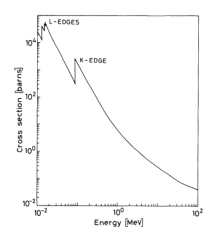
\includegraphics{./figures/photoeffekt.png}
	\caption{Wirkungsquerschnitt für den Photoeffekt an Blei. QUELLE William R. Leo}
	\label{fig:photoeffekt}
\end{figure}

\subsubsection{Compton-Effekt}
Der Compton-Effekt beschreibt die Streuung von Photonen an freien Elektronen.
Allerdings können Elektronen im Fall $E_\gamma \gg E_\mathrm{Bind. e^{-}}$ auch in Materie als frei betrachtet werden.
Die Streuung beschreibt einen winkelabhängigen Energieübertrag vom Photon auf das Elektron, wobei der Streuwinkel $\theta$ des Photons relativ zur einfallenden Flugrichtung angegeben wird.
\begin{figure}
	\centering
	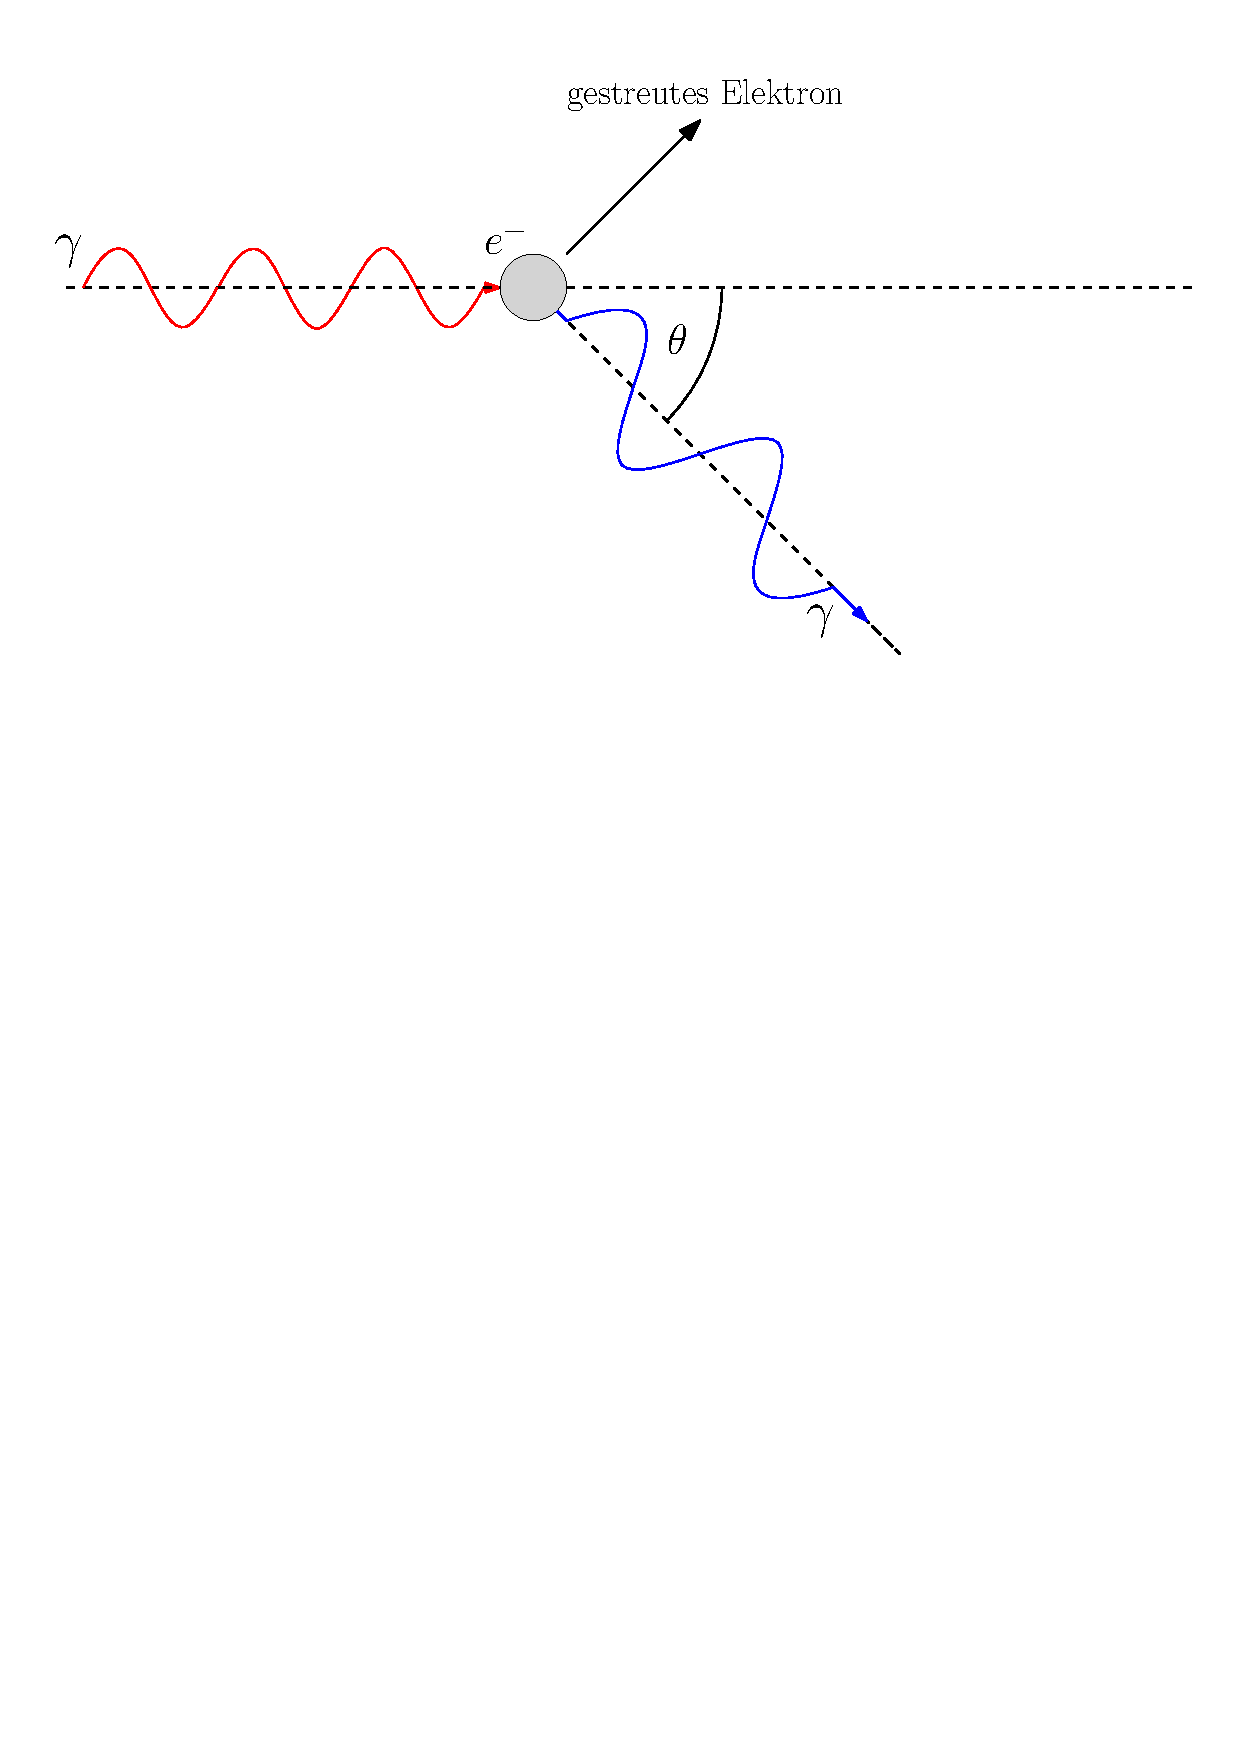
\includegraphics[width=0.8\textwidth]{./figures/compton.pdf}
	\caption{Comptoneffekt}
	\label{fig:comptoneffekt}
\end{figure}
\begin{align}
	\frac{E_\gamma^\prime}{E_\gamma} &= \frac{1}{1 + \frac{h \nu}{m_\mathrm{e} c^2} (1-\cos\theta)} \\
	\Delta \lambda &= \lambda_\mathrm{c} (1 - \cos\theta) \\
	\lambda_\mathrm{c} &= \frac{h}{m_\mathrm{e} c}
\end{align}
Wirkungsquerschnitt gegeben durch Klein-Nishina:
\begin{align}
	\sigma_\mathrm{c} \propto \frac{Z}{E_\gamma}
\end{align}

Compton-Kante...

Kein Energietransfer:\\
Thomson-Streuung: Compton im klassischen Limit\\
Rayleigh-Streuung: Streuung am ganzen Atom\\


\subsubsection{Paarbildung}
\begin{align}
	\gamma \rightarrow \mathrm{e}^{+} + \mathrm{e}^{-}\\
	E_\gamma \geq 2 m_\mathrm{e} c^2
\end{align}

\begin{align}
	\sigma_\mathrm{Paar} \propto Z^2 \ln E_\gamma
\end{align}

\subsubsection{Summe aller Effekte}

Bildah

\subsection{Szintillatoren, Halbleiterdetektor, Photomulti etc.}

\subsubsection{Detektor Charakteristiken}
Output des Detektors ein Strompuls und die Energie des detektierten Teilchens ist proportional zu der Ladung des Pulses.
Ist die Pulsform von Teilchen verschiedener Energien immer gleich, so ist dies gleichbedeutend zu der Höhe des Pulses.\\
\\
Energieauflösung: Linien haben Gaußform. Weite der Linie verursacht durch Fluktuationen in der Anzahl der Ionisationen/Anregungen(Poissonverteilt) (statistischer Prozess: $\mathcal{R} \propto 1 / \sqrt{N}$ mit der Anzahl der Ionisationen bei gegebener Energie $N$. Zentraler Grenzwertsatz: $\sigma_x^2 / \braket{X} \propto 1 / \sqrt{N}$, wobei X eine Summe von N Zufallsvariablen ist.).
Auflösung (FWHM):
\begin{align}
	\text{Resolution} = \frac{\Delta E}{E}
\end{align}
Auflösung ist eine Funktion der Energie! Generell ist die Anzahl der Ionisationen proportional zur Energie des einfallenden Teilchens. Damit skaliert die Auflösung ebenfalls wie:
\begin{align}
	\mathcal{R} \propto \frac{1}{\sqrt{E_\gamma}}
\end{align}
Neben der intrinsischen Unschärfe des Detektors kommt noch Unschärfe der verwendeten Elektron, welche sich quadratisch addiert:
\begin{align}
	\Delta E^2 = \Delta E_\mathrm{Detektor}^2 + \Delta E_\mathrm{Elektronik}^2
\end{align}
\\
Detektoreffizienz: Unterscheidung zwischen absoluter und intrinsischer Effizienz.\\
Absolute (totale) Effizienz:
\begin{align}
	\mathcal{E}_\mathrm{tot} = \frac{\text{events registered}}{\text{events emitted by source}}
\end{align}
(Peakeffizienz: events registered $\rightarrow$ Ereignisse im Photopeak) 
Ist abhängig von der Detektorgeometrie und der Wahrscheinlichkeit einer Interaktion mit dem Detektor.\\
\\
Intrinsische Effizienz:
\begin{align}
	\mathcal{E}_\mathrm{int} = \frac{\text{events registered}}{\text{events impinging on detector}}
\end{align}
Mit der absoluten Peakeffizienz scheint die intrinsische Effizienz aus Leo gemeint zu sein.
\begin{align}
	\label{eq:peakeffizienz}
	\mathcal{E}_\mathrm{int} = \frac{N_\mathrm{Photo.}}{A \cdot T \cdot \frac{\pi r^2}{4\pi \, d^2}}
\end{align}
Der geometrische Faktor im Nenner geht von einer Punktquelle (Aktivität $A$) in hohem Abstand vom Detektor $d$ aus. Messzeit $T$, Detektorradius $r$.

\subsubsection{Szintillatoren}
Szintillator: Körper dessen Moleküle beim Durchgang von energiereichen Photonen angeregt werden und folglich Licht (meist im UV-Bereich) emittieren. In Kombination mit Photomulti geeignete Detektoren.\\
\\
Über einer Mindestenergie verhalten sich Szintillatoren linear (Lichtenerzeugung - Energie des Photons)
\\
Besteht aus Kristall mit Aktivator-Zentren (Dotierung)\\
Einfallendes Photon löst $\mathrm{e}^{-}$-Kaskade aus bis Energie klein genug ist um wieder in Atomen gefangen zu werden $\rightarrow$ Photonenemission\\
Kristall selber ist nicht transparent für diese Photonen. Dotierung erzeugt neue Energieniveaus, über welche Photonen erzeugt werden für die das Material transparent ist.\\
Oft mit Thallium aktivierte NaI-Kristalle wegen der hohen Ordnungszahl von Jod(Iod).\\
\\
Exciton: Unreinheiten im Kristall verursachen ein Exciton-Band unter dem Leitungsband. Ein einfallendes Photon erzeugt nur ein Exciton (e-Loch-Paar) im Exciton-Band/Valenzband, welches frei im Kristall beweglich ist. Trifft dieses Exciton auf eine Verunreinigung (Thallium) kann dieses durch das Loch des Excitons ionisiert werden und das Exciton über ein lokales Energieniveau aufgrund der Verunreinigung abgeregt werden (unter Emission von Photonen).\\
\\
Für die Detektion von Photonen sind hohe Ordnungszahlen $Z$ wünscheswert (vgl. Wirkungsquerschnitt Photoeffekt im vergleich zu Compton)

\subsubsection{Halbleiterdetektor}
Analog zum Gas-Ionisationsdetektor nur dass Elektronen-Loch Paare statt Elektron-Ion-Paare erzeugt werden.
Vorteil: Erzeugung von e-Loch-Paar benötigt weniger Energie (Bandlücke); dadurch mehr Paare.\\
\\
Höhere Dichte höhere stopping-power (mehr Energiedeposition).\\
\\
Kompakt und hohe response time.\\
\\
Außer Silizium benötigen sie Kühlung da thermische e-Loch-Paare erzeugt werden können. Größter Faktor aber trotzdem Oberflächenströme, daher wird ein gut verkapselter Detektor benötigt.\\
\\
Rekombination in Halbleitern ist selten, da Loch und Elektron Impuls und Energieerhaltung erfüllen müssen(Lebenszeiten Größenordnung Sekunde).
Rekombinationszentren: Verunreinigung sorgen für weitere Energieniveaus zwischen Valenz und Leitungsband, welche ein Elektron einfangen können. Folge: a) Das Elektron geht wieder in das Leitungsband. b) Nach einer Zeit trifft auf die Verunreinigung ein Loch, welches mit dem gefangenen Elektron annhiliert.
Es folgt das Halbleiterdetektoren sehr reine Kristalle benötigt, da die Ladung an den Kathoden eingefangen werden soll.\\
\\
Trapping: Verunreinheiten die nur einen Typ von Ladungsträger (Elektron, Loch) einfangen können und diese für eine gewisse Zeit halten und danach wieder freigeben. Negativer Einfluss auf die Ladungssammlung.
Ähnlicher Effekt durch Gitterdefekte.\\
\\
PN-Übergang in reverse Bias. In der Verarmungszone werden Elektron-Loch-Paare erzeugt (durch ionisierende Strahlung) die als Strompuls gemessen werden können. Reverse Bias: 1) Verarmungszone ist größer dadurch wird mehr Strahlung detektiert 2) Feld in der Verarmungszone ist größer und begünstigt die Ladungssammlung. An den Metallkontakten muss der Halbleiter stark dotiert sein um einen ohmschen Übergang zu erlauben. (sonst wirkt er wie eine Diode)\\
\\
Energie für e-Loch-Bildung:
\begin{align}
	E_\mathrm{Ge} = \SI{2.96}{eV} \quad \text{@ 77 K}
\end{align}
Mehr als Bandlücke da ein Teil der Energie in Anregungen des Gitter übergeht.
Cite William R. Leo\\
Im Vergleich zur Photoelektronenbildung in Szintillatoren zwei Größenordnung höhere e-Loch-Bildung und damit bessere Energieauflösung.\\
\\
Aufgrund der hohen Ordnungszahl von Germanium ist der Photowirkungsquerschnitt 60 mal größer als der von Silizium.\\
Vergleich von Germanium und NaI-Detektor im Leo Fig. 10{.}19.

\subsection{Spektrum, Vielkanalanalysator}

\subsection{Auflösungsvermögen, Breite, Unterschiede der Detektoren}

\subsection{Nachweiswahrscheinlichkeit}

\subsection{Termschemata}


\section{Versuchsaufbau}

\section{Durchführung und Auswertung}
Die ausführliche Durchführung ist der Versuchsanleitung \cite{anleitung} zu entnehmen.
Sollten Abweichungen bei der Durchführung auftreten, so werden diese im jeweiligen Unterkapitel dargestellt.

\subsection{NaI(Tl) Szintillationsspektrometer}
Es wird der Detektor mit Durchmesser \SI{48}{mm} verwendet. (????)


\subsubsection{Detektorsignal des Szintillationsdetektors}
\label{sec:detektorsignal_szinti}
In diesem Abschnitt soll das Signalverhalten des verwendeten NaI(Tl)-Szintillationsdetektors untersucht werden.
Dazu wurden mit einem Oszilloskop die Signalformen jeweils am Vorverstärker des Photomultipliers sowie am Hauptverstärker aufgenommen.
In Abbildung \ref{fig:signal_szinti_vor} ist ein beispielhaftes Signal direkt am Vorverstärker dargestellt.
\begin{figure}[h]
	\centering
	\begin{subfigure}[b]{0.7\textwidth}
		\centering
		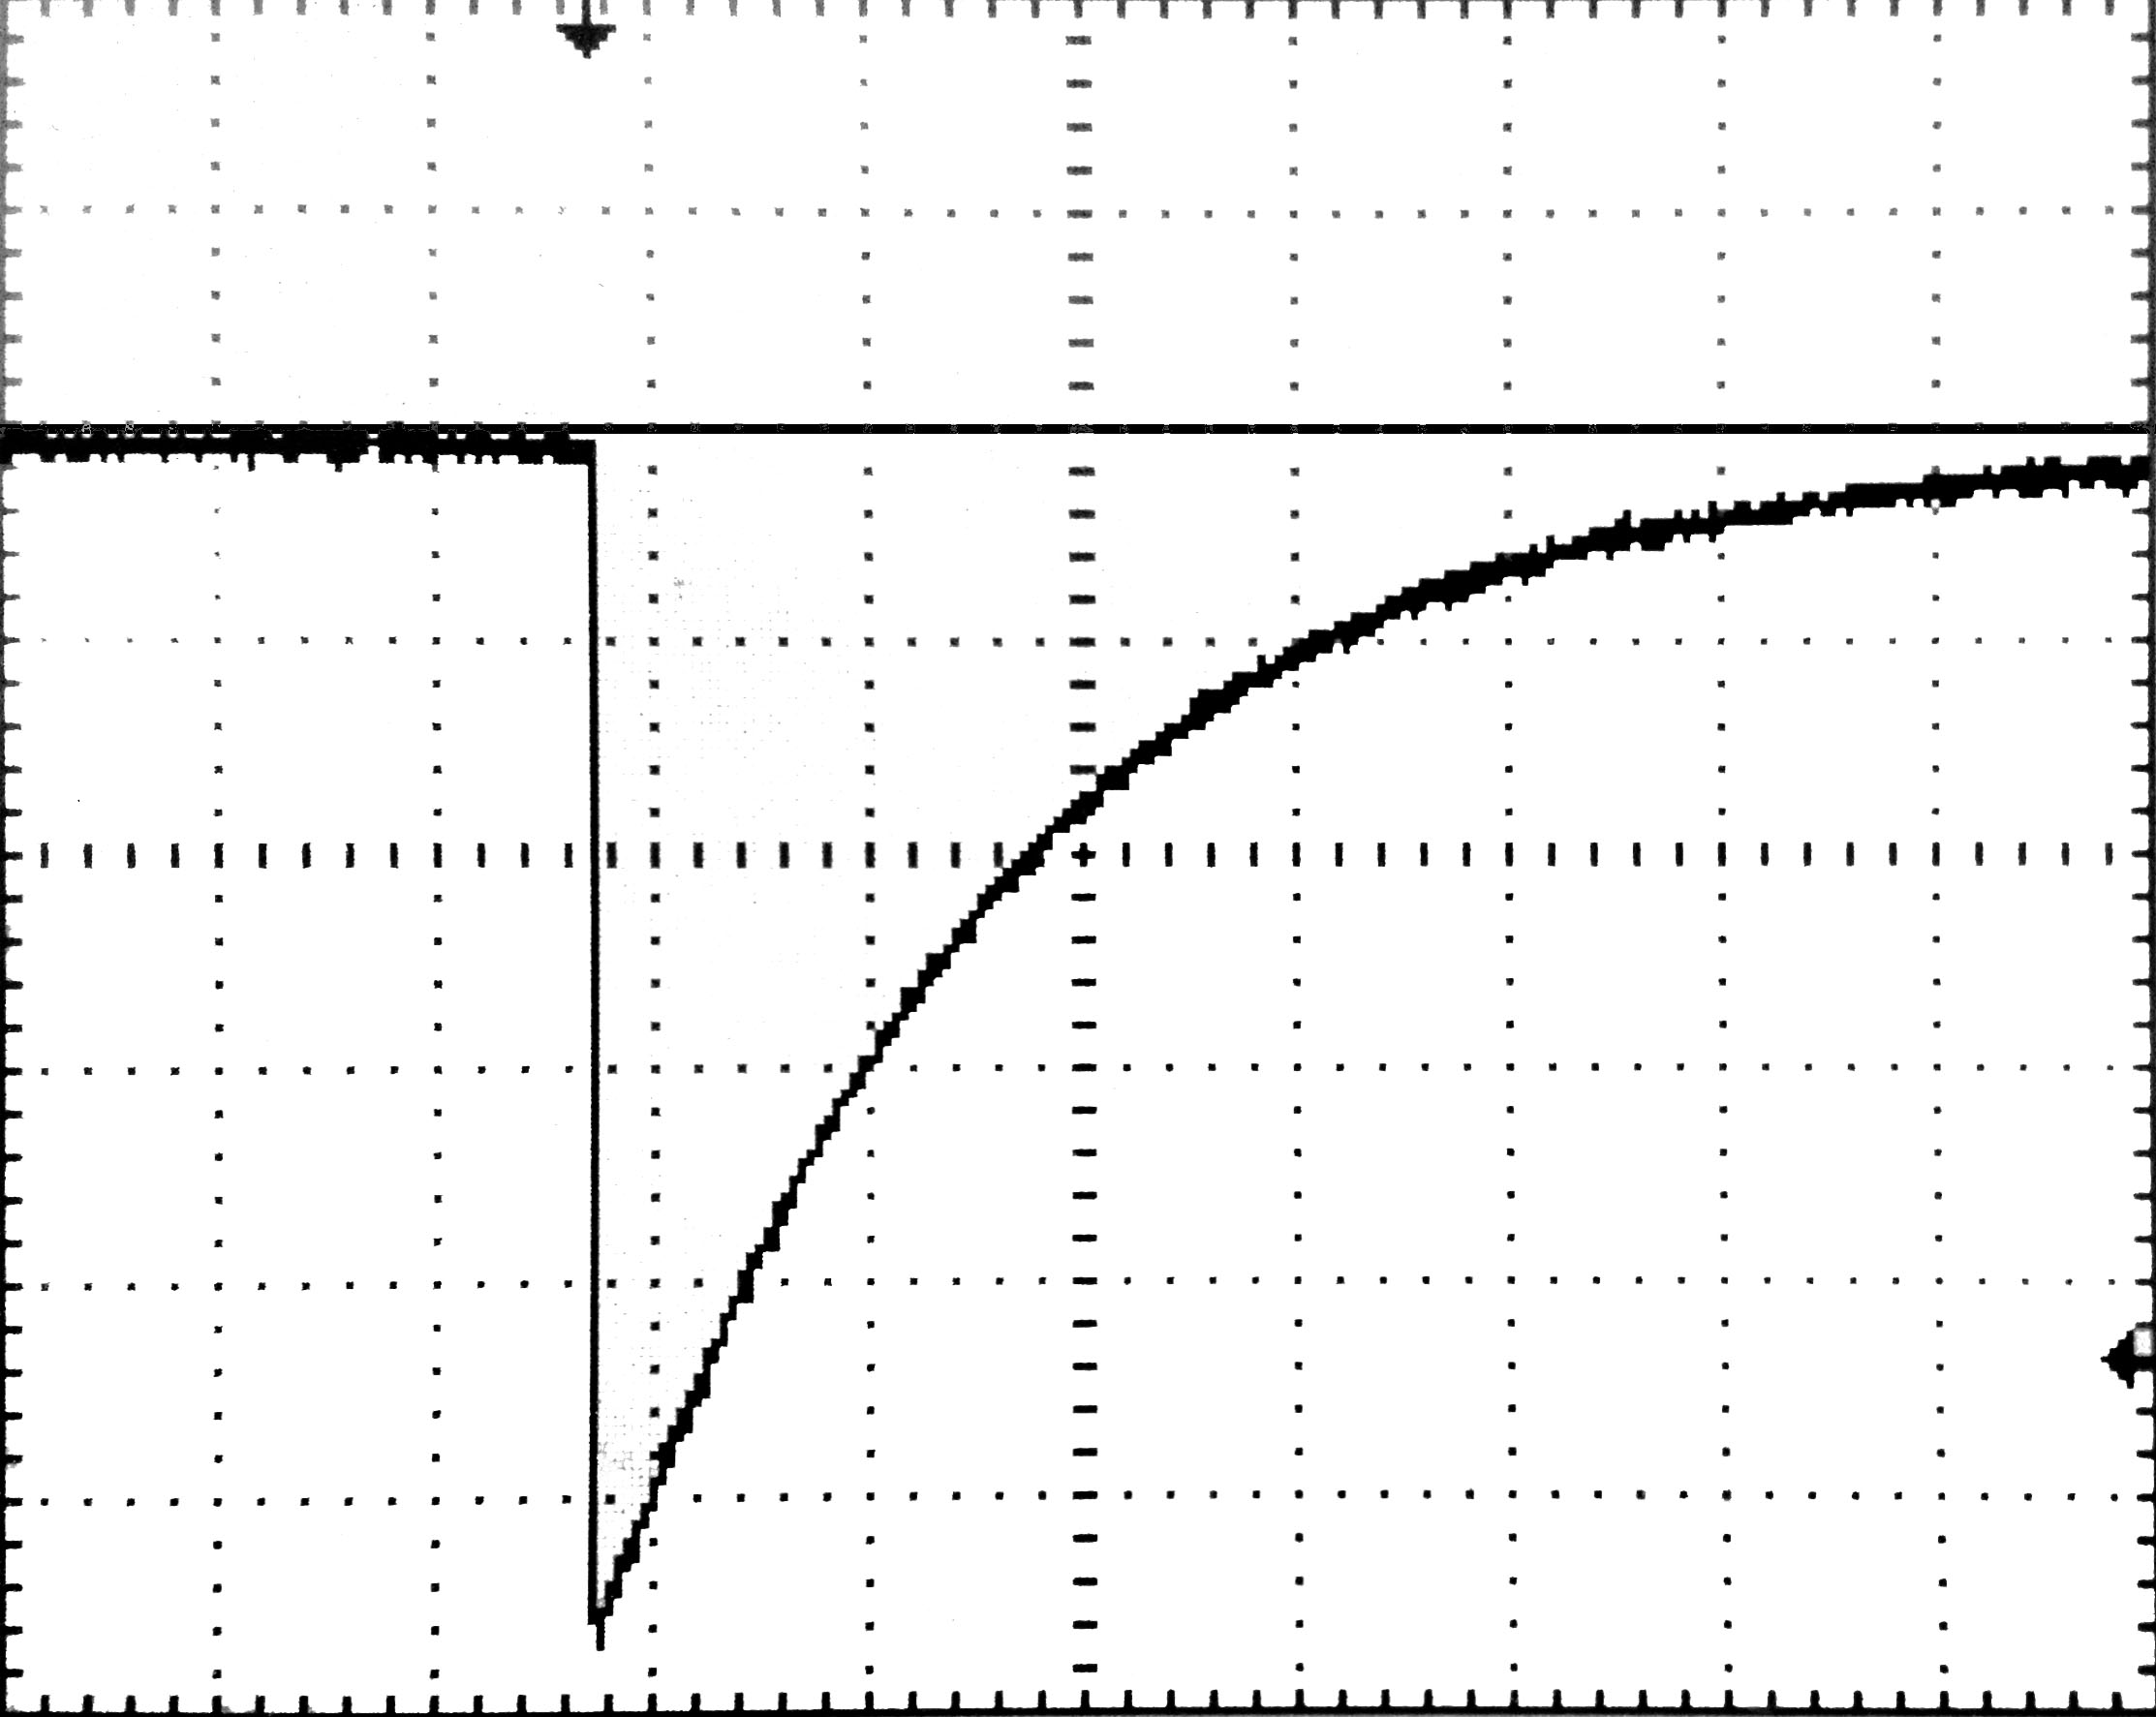
\includegraphics[width=0.7\textwidth]{./figures/signale/vor_szinti_abgeschnitten.jpg}
		\caption{Am Ausgang des Vorverstärkers des Photomultipliers. Die eingestellten Skalenfaktoren am Oszilloskop betragen \SI{0.5}{\volt\per\division} für die Vertikale und \SI{100}{\micro\second\per\division} in der Horizontalen.}
		\label{fig:signal_szinti_vor}
	\end{subfigure}
	
	\begin{subfigure}[b]{0.7\textwidth}
		\centering
		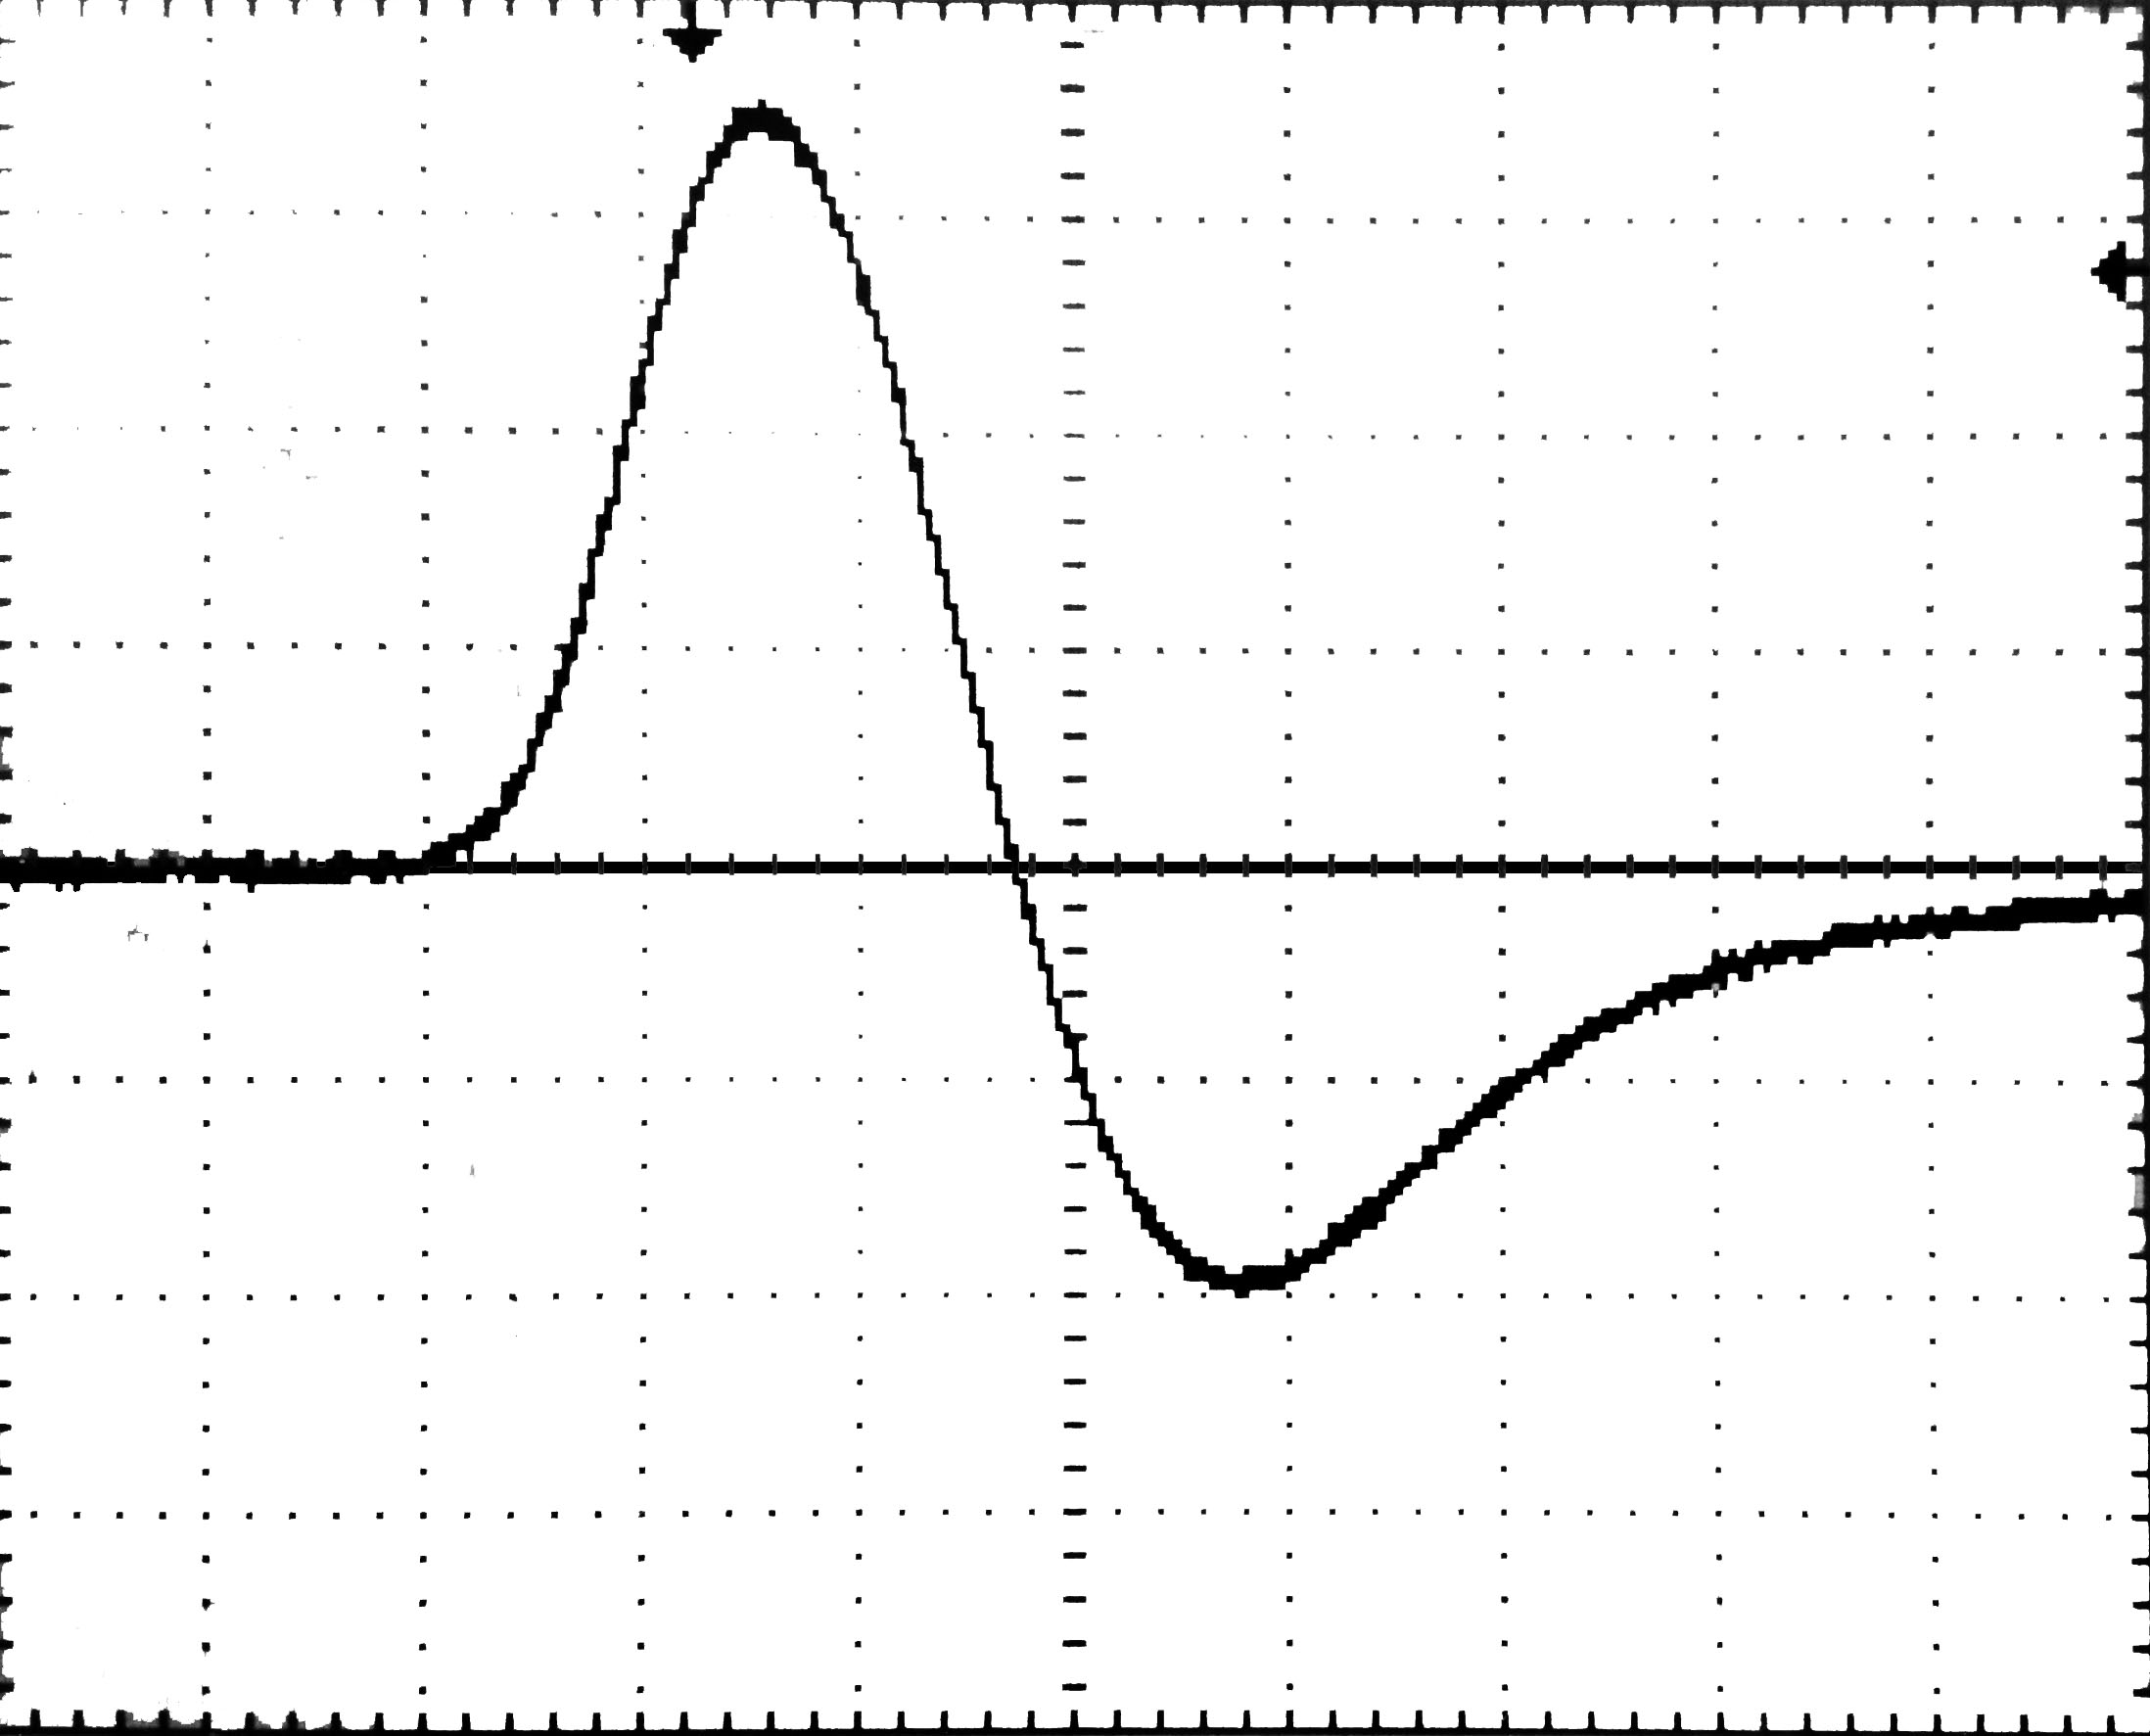
\includegraphics[width=0.7\textwidth]{./figures/signale/haupt_szinti_abgeschnitten.jpg}
		\caption{Am Ausgang des Hauptverstärkers. Die eingestellten Skalenfaktoren am Oszilloskop betragen \SI{1}{\volt\per\division} für die Vertikale und \SI{1}{\micro\second\per\division} in der Horizontalen.}
		\label{fig:signal_szinti_haupt}
	\end{subfigure}
	\caption{Signalformen am Szintillationsdetektor. Die horizontalen Linien markieren \SI{0}{\volt}.}
\end{figure}
Die im Folgenden gemessenen Größen wurden mithilfe eines Bildbearbeitungsprogrammes direkt an den Aufnahmen des Oszilloskops abgemessen.
Dabei wurden die Fehler auf \SI{0.2}{\division} der jeweiligen Spannungs-/Zeitskala abgeschätzt.
Das Signal am Vorverstärker des Photomultipliers weist einen (im Vergleich zur Signaldauer) instantanen Anstieg (Anstiegszeit $< \SI{5}{\micro\second}$) mit der Signalamplitude $\Delta U = \SI{2.8 +- 0.1}{\volt}$ auf.
Nach diesem Anstieg fällt das Signal exponentiell mit einer Signaldauer\footnote{Als Definition der Signaldauer $\Delta t$ wird dabei die Zeit verwendet, die das Signal benötigt um von \SI{10}{\percent} der Signalamplitude an der ansteigenden Flanke auf \SI{10}{\percent} an der abfallenden Flanke zu gelangen.} von $\Delta t = \SI{395 +- 20}{\micro\second}$ ab.
Der exponentielle Abfall des Signals kann durch den relativ langsamen Abtransport der Ladung im Sekundarelektronenvervielfacher erklärt werden.
Im Vergleich dazu wurde in Abbildung \ref{fig:signal_szinti_haupt} eines der Signale am Hauptverstärker des Detektors dargestellt.
Obwohl der Puls am unipolaren Ausgang des Verstärkers gemessen wurde, kann ein negativer Ausschlag festgestellt werden.
Der negative Impuls ist für die Messung nicht relevant, da dieser bei der Impulshöhenmessung mit dem Vielkanalanalysator keinen Einfluss hat.
Der für die Messung relevante positive Impuls hat eine Amplitude von $\Delta U = \SI{3.4 +- 0.2}{\volt}$ und eine Signaldauer $\Delta t = \SI{2.3 +- 0.2}{\micro\second}$.
Der Vergleich der Amplituden\footnote{Ein direkter Vergleich der beiden Signale macht nur Sinn, wenn lediglich Größenordnungen betrachtet werden, da die beiden Signale von unabhängigen Ereignissen stammen.} an beiden Verstärkern legt nahe, dass der Hauptverstärker nicht zur Verstärkung der Spannung dient sondern vielmehr zur Impulsformung.
Dies sieht man besonders an der um zwei Größenordnungen verkürzten Signaldauer.
Da beide Signale von unabhängigen Ereignissen stammen, kann leider nicht verifiziert werden, dass die Impulshöhe am Hauptverstärker proportional zur im Photomultiplier gelösten Ladung, ist, welche wiederum proportional zur Fläche über dem Signal am Vorverstärker ist.

\subsubsection{Aufnahme der Gammaspektren von QUELLEN und das Untergrundspektrum}
Nachdem die Signale des Szintillationsdetektors betrachtet wurden, kann mit der Aufnahme der Spektren begonnen werden.
Dazu muss die Verstärkung des Hauptverstärkers geeignet eingestellt werden, um den Kanalbereich des Vielkanalanalysators optimal auszunutzen.
Dies wird dadurch erreicht, dass die hochenergetische \SI{1408}{keV}-Linie von \isotope[152]{Eu} über die Verstärkung so positioniert wird, dass diese in den Bereich um Kanal 7000 fällt.
Anschließend wird ein Untergrundspektrum aufgenommen, um die Spektren der Isotope \isotope[60]{Co}, \isotope[137]{Cs} und \isotope[152]{Eu} vom Untergrund bereinigen zu können.
Die Messzeit beträgt für alle Spektrenaufnahmen \SI{720}{\second}.
Generell wird für den Fehler auf die Anzahl der Ereignisse $N$ in einem bestimmten Kanal $n$ des Vielkanalanalysators wegen der zugrundeliegenden Poisson-Verteilung:
\begin{align}
\label{eq:poisson_fehler}
\Delta N = \sqrt{N}
\end{align}
angenommen.
Das Untergrundspektrum wie auch die Spektren der verschiedenen Isotope wurden über eine Messdauer von $t = \SI{720}{\second}$ aufgenommen.
Die Untergrundkorrektur erfolgt dann durch Subtraktion des Untergrundspektrums von den aufgenommenen Spektren der Isotope:
\begin{align}
	\label{eq:untergrundkorr_fehler}
	N_\mathrm{korr.} &= N - N_\mathrm{Untergrund}  \nonumber\\
	\Delta N_\mathrm{korr.} &= \sqrt{\Delta N^2 + \Delta N_\mathrm{Untergrund}^2} = \sqrt{N + N_\mathrm{Untergrund}}
\end{align}
wobei der Fehler aufgrund von Gleichung \ref{eq:poisson_fehler} und Gauß'scher Fehlerfortpflanzung folgt.
Aus Gründen der Übersichtlichkeit wurde in Abbildung \ref{fig:abzug_untergrund} der Abzug des Untergrundes am Beispiel der Messung von \isotope[60]{Co} durchgeführt und im Folgenden nur noch die vom Untergrund bereinigten Spektren abgebildet.
\begin{figure}[hp]
	\centering
	\begin{subfigure}[b]{0.65\textwidth}
		\resizebox{!}{0.285\textheight}{
		% GNUPLOT: LaTeX picture with Postscript
\begingroup
  \makeatletter
  \providecommand\color[2][]{%
    \GenericError{(gnuplot) \space\space\space\@spaces}{%
      Package color not loaded in conjunction with
      terminal option `colourtext'%
    }{See the gnuplot documentation for explanation.%
    }{Either use 'blacktext' in gnuplot or load the package
      color.sty in LaTeX.}%
    \renewcommand\color[2][]{}%
  }%
  \providecommand\includegraphics[2][]{%
    \GenericError{(gnuplot) \space\space\space\@spaces}{%
      Package graphicx or graphics not loaded%
    }{See the gnuplot documentation for explanation.%
    }{The gnuplot epslatex terminal needs graphicx.sty or graphics.sty.}%
    \renewcommand\includegraphics[2][]{}%
  }%
  \providecommand\rotatebox[2]{#2}%
  \@ifundefined{ifGPcolor}{%
    \newif\ifGPcolor
    \GPcolortrue
  }{}%
  \@ifundefined{ifGPblacktext}{%
    \newif\ifGPblacktext
    \GPblacktexttrue
  }{}%
  % define a \g@addto@macro without @ in the name:
  \let\gplgaddtomacro\g@addto@macro
  % define empty templates for all commands taking text:
  \gdef\gplbacktext{}%
  \gdef\gplfronttext{}%
  \makeatother
  \ifGPblacktext
    % no textcolor at all
    \def\colorrgb#1{}%
    \def\colorgray#1{}%
  \else
    % gray or color?
    \ifGPcolor
      \def\colorrgb#1{\color[rgb]{#1}}%
      \def\colorgray#1{\color[gray]{#1}}%
      \expandafter\def\csname LTw\endcsname{\color{white}}%
      \expandafter\def\csname LTb\endcsname{\color{black}}%
      \expandafter\def\csname LTa\endcsname{\color{black}}%
      \expandafter\def\csname LT0\endcsname{\color[rgb]{1,0,0}}%
      \expandafter\def\csname LT1\endcsname{\color[rgb]{0,1,0}}%
      \expandafter\def\csname LT2\endcsname{\color[rgb]{0,0,1}}%
      \expandafter\def\csname LT3\endcsname{\color[rgb]{1,0,1}}%
      \expandafter\def\csname LT4\endcsname{\color[rgb]{0,1,1}}%
      \expandafter\def\csname LT5\endcsname{\color[rgb]{1,1,0}}%
      \expandafter\def\csname LT6\endcsname{\color[rgb]{0,0,0}}%
      \expandafter\def\csname LT7\endcsname{\color[rgb]{1,0.3,0}}%
      \expandafter\def\csname LT8\endcsname{\color[rgb]{0.5,0.5,0.5}}%
    \else
      % gray
      \def\colorrgb#1{\color{black}}%
      \def\colorgray#1{\color[gray]{#1}}%
      \expandafter\def\csname LTw\endcsname{\color{white}}%
      \expandafter\def\csname LTb\endcsname{\color{black}}%
      \expandafter\def\csname LTa\endcsname{\color{black}}%
      \expandafter\def\csname LT0\endcsname{\color{black}}%
      \expandafter\def\csname LT1\endcsname{\color{black}}%
      \expandafter\def\csname LT2\endcsname{\color{black}}%
      \expandafter\def\csname LT3\endcsname{\color{black}}%
      \expandafter\def\csname LT4\endcsname{\color{black}}%
      \expandafter\def\csname LT5\endcsname{\color{black}}%
      \expandafter\def\csname LT6\endcsname{\color{black}}%
      \expandafter\def\csname LT7\endcsname{\color{black}}%
      \expandafter\def\csname LT8\endcsname{\color{black}}%
    \fi
  \fi
    \setlength{\unitlength}{0.0500bp}%
    \ifx\gptboxheight\undefined%
      \newlength{\gptboxheight}%
      \newlength{\gptboxwidth}%
      \newsavebox{\gptboxtext}%
    \fi%
    \setlength{\fboxrule}{0.5pt}%
    \setlength{\fboxsep}{1pt}%
\begin{picture}(7200.00,5040.00)%
    \gplgaddtomacro\gplbacktext{%
      \csname LTb\endcsname%
      \put(814,704){\makebox(0,0)[r]{\strut{}$0$}}%
      \csname LTb\endcsname%
      \put(814,1518){\makebox(0,0)[r]{\strut{}$50$}}%
      \csname LTb\endcsname%
      \put(814,2332){\makebox(0,0)[r]{\strut{}$100$}}%
      \csname LTb\endcsname%
      \put(814,3147){\makebox(0,0)[r]{\strut{}$150$}}%
      \csname LTb\endcsname%
      \put(814,3961){\makebox(0,0)[r]{\strut{}$200$}}%
      \csname LTb\endcsname%
      \put(814,4775){\makebox(0,0)[r]{\strut{}$250$}}%
      \csname LTb\endcsname%
      \put(946,484){\makebox(0,0){\strut{}$0$}}%
      \csname LTb\endcsname%
      \put(1597,484){\makebox(0,0){\strut{}$1000$}}%
      \csname LTb\endcsname%
      \put(2248,484){\makebox(0,0){\strut{}$2000$}}%
      \csname LTb\endcsname%
      \put(2898,484){\makebox(0,0){\strut{}$3000$}}%
      \csname LTb\endcsname%
      \put(3549,484){\makebox(0,0){\strut{}$4000$}}%
      \csname LTb\endcsname%
      \put(4200,484){\makebox(0,0){\strut{}$5000$}}%
      \csname LTb\endcsname%
      \put(4851,484){\makebox(0,0){\strut{}$6000$}}%
      \csname LTb\endcsname%
      \put(5501,484){\makebox(0,0){\strut{}$7000$}}%
      \csname LTb\endcsname%
      \put(6152,484){\makebox(0,0){\strut{}$8000$}}%
      \csname LTb\endcsname%
      \put(6803,484){\makebox(0,0){\strut{}$9000$}}%
    }%
    \gplgaddtomacro\gplfronttext{%
      \csname LTb\endcsname%
      \put(176,2739){\rotatebox{-270}{\makebox(0,0){\strut{}Ereignisse $$}}}%
      \put(3874,154){\makebox(0,0){\strut{}Kanal $n$}}%
      \csname LTb\endcsname%
      \put(5816,4602){\makebox(0,0)[r]{\strut{}Messwerte}}%
    }%
    \gplbacktext
    \put(0,0){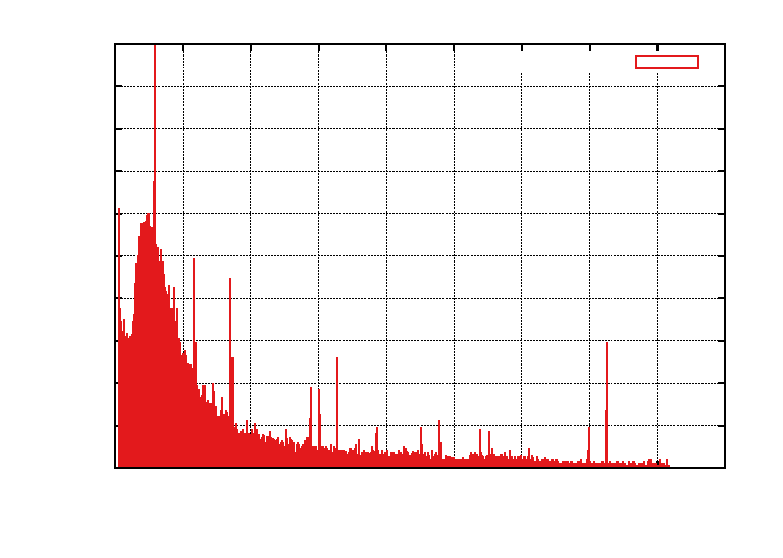
\includegraphics{./plots/halbleiter/untergrund}}%
    \gplfronttext
  \end{picture}%
\endgroup

		}
		\caption{Untergrund des NaI(Tl)-Szintillationsdetektors}
		\label{fig:untergrund_szinti}
	\end{subfigure}
	
	\begin{subfigure}[b]{0.65\textwidth}
		\resizebox{!}{0.285\textheight}{
		% GNUPLOT: LaTeX picture with Postscript
\begingroup
  \makeatletter
  \providecommand\color[2][]{%
    \GenericError{(gnuplot) \space\space\space\@spaces}{%
      Package color not loaded in conjunction with
      terminal option `colourtext'%
    }{See the gnuplot documentation for explanation.%
    }{Either use 'blacktext' in gnuplot or load the package
      color.sty in LaTeX.}%
    \renewcommand\color[2][]{}%
  }%
  \providecommand\includegraphics[2][]{%
    \GenericError{(gnuplot) \space\space\space\@spaces}{%
      Package graphicx or graphics not loaded%
    }{See the gnuplot documentation for explanation.%
    }{The gnuplot epslatex terminal needs graphicx.sty or graphics.sty.}%
    \renewcommand\includegraphics[2][]{}%
  }%
  \providecommand\rotatebox[2]{#2}%
  \@ifundefined{ifGPcolor}{%
    \newif\ifGPcolor
    \GPcolortrue
  }{}%
  \@ifundefined{ifGPblacktext}{%
    \newif\ifGPblacktext
    \GPblacktexttrue
  }{}%
  % define a \g@addto@macro without @ in the name:
  \let\gplgaddtomacro\g@addto@macro
  % define empty templates for all commands taking text:
  \gdef\gplbacktext{}%
  \gdef\gplfronttext{}%
  \makeatother
  \ifGPblacktext
    % no textcolor at all
    \def\colorrgb#1{}%
    \def\colorgray#1{}%
  \else
    % gray or color?
    \ifGPcolor
      \def\colorrgb#1{\color[rgb]{#1}}%
      \def\colorgray#1{\color[gray]{#1}}%
      \expandafter\def\csname LTw\endcsname{\color{white}}%
      \expandafter\def\csname LTb\endcsname{\color{black}}%
      \expandafter\def\csname LTa\endcsname{\color{black}}%
      \expandafter\def\csname LT0\endcsname{\color[rgb]{1,0,0}}%
      \expandafter\def\csname LT1\endcsname{\color[rgb]{0,1,0}}%
      \expandafter\def\csname LT2\endcsname{\color[rgb]{0,0,1}}%
      \expandafter\def\csname LT3\endcsname{\color[rgb]{1,0,1}}%
      \expandafter\def\csname LT4\endcsname{\color[rgb]{0,1,1}}%
      \expandafter\def\csname LT5\endcsname{\color[rgb]{1,1,0}}%
      \expandafter\def\csname LT6\endcsname{\color[rgb]{0,0,0}}%
      \expandafter\def\csname LT7\endcsname{\color[rgb]{1,0.3,0}}%
      \expandafter\def\csname LT8\endcsname{\color[rgb]{0.5,0.5,0.5}}%
    \else
      % gray
      \def\colorrgb#1{\color{black}}%
      \def\colorgray#1{\color[gray]{#1}}%
      \expandafter\def\csname LTw\endcsname{\color{white}}%
      \expandafter\def\csname LTb\endcsname{\color{black}}%
      \expandafter\def\csname LTa\endcsname{\color{black}}%
      \expandafter\def\csname LT0\endcsname{\color{black}}%
      \expandafter\def\csname LT1\endcsname{\color{black}}%
      \expandafter\def\csname LT2\endcsname{\color{black}}%
      \expandafter\def\csname LT3\endcsname{\color{black}}%
      \expandafter\def\csname LT4\endcsname{\color{black}}%
      \expandafter\def\csname LT5\endcsname{\color{black}}%
      \expandafter\def\csname LT6\endcsname{\color{black}}%
      \expandafter\def\csname LT7\endcsname{\color{black}}%
      \expandafter\def\csname LT8\endcsname{\color{black}}%
    \fi
  \fi
    \setlength{\unitlength}{0.0500bp}%
    \ifx\gptboxheight\undefined%
      \newlength{\gptboxheight}%
      \newlength{\gptboxwidth}%
      \newsavebox{\gptboxtext}%
    \fi%
    \setlength{\fboxrule}{0.5pt}%
    \setlength{\fboxsep}{1pt}%
\begin{picture}(7200.00,5040.00)%
    \gplgaddtomacro\gplbacktext{%
      \csname LTb\endcsname%
      \put(946,704){\makebox(0,0)[r]{\strut{}$0$}}%
      \csname LTb\endcsname%
      \put(946,1111){\makebox(0,0)[r]{\strut{}$100$}}%
      \csname LTb\endcsname%
      \put(946,1518){\makebox(0,0)[r]{\strut{}$200$}}%
      \csname LTb\endcsname%
      \put(946,1925){\makebox(0,0)[r]{\strut{}$300$}}%
      \csname LTb\endcsname%
      \put(946,2332){\makebox(0,0)[r]{\strut{}$400$}}%
      \csname LTb\endcsname%
      \put(946,2740){\makebox(0,0)[r]{\strut{}$500$}}%
      \csname LTb\endcsname%
      \put(946,3147){\makebox(0,0)[r]{\strut{}$600$}}%
      \csname LTb\endcsname%
      \put(946,3554){\makebox(0,0)[r]{\strut{}$700$}}%
      \csname LTb\endcsname%
      \put(946,3961){\makebox(0,0)[r]{\strut{}$800$}}%
      \csname LTb\endcsname%
      \put(946,4368){\makebox(0,0)[r]{\strut{}$900$}}%
      \csname LTb\endcsname%
      \put(946,4775){\makebox(0,0)[r]{\strut{}$1000$}}%
      \csname LTb\endcsname%
      \put(1078,484){\makebox(0,0){\strut{}$0$}}%
      \csname LTb\endcsname%
      \put(1794,484){\makebox(0,0){\strut{}$1000$}}%
      \csname LTb\endcsname%
      \put(2509,484){\makebox(0,0){\strut{}$2000$}}%
      \csname LTb\endcsname%
      \put(3225,484){\makebox(0,0){\strut{}$3000$}}%
      \csname LTb\endcsname%
      \put(3941,484){\makebox(0,0){\strut{}$4000$}}%
      \csname LTb\endcsname%
      \put(4656,484){\makebox(0,0){\strut{}$5000$}}%
      \csname LTb\endcsname%
      \put(5372,484){\makebox(0,0){\strut{}$6000$}}%
      \csname LTb\endcsname%
      \put(6087,484){\makebox(0,0){\strut{}$7000$}}%
      \csname LTb\endcsname%
      \put(6803,484){\makebox(0,0){\strut{}$8000$}}%
    }%
    \gplgaddtomacro\gplfronttext{%
      \csname LTb\endcsname%
      \put(176,2739){\rotatebox{-270}{\makebox(0,0){\strut{}Ereignisse $N$}}}%
      \put(3940,154){\makebox(0,0){\strut{}Kanal $n$}}%
      \csname LTb\endcsname%
      \put(2398,4602){\makebox(0,0)[r]{\strut{}Messwerte}}%
    }%
    \gplbacktext
    \put(0,0){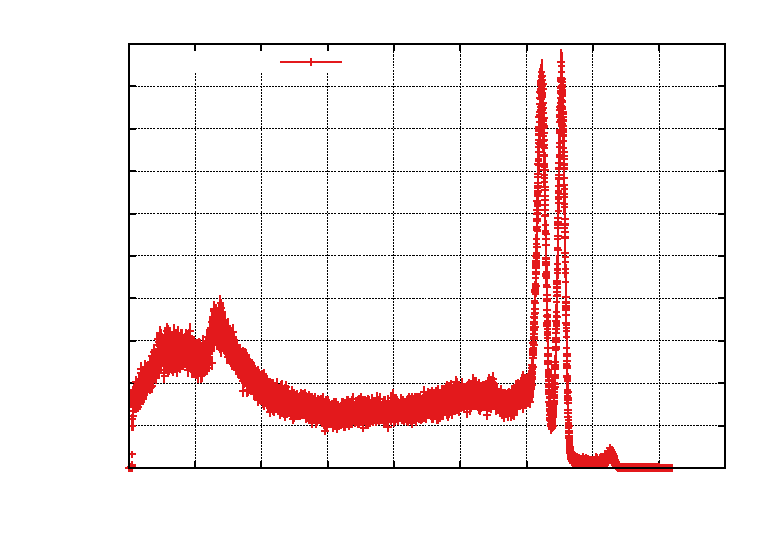
\includegraphics{./plots/szintillator/cobalt_mit_untergrund}}%
    \gplfronttext
  \end{picture}%
\endgroup

		}
		\caption{Untergrundbehaftetes \isotope[60]{Co}-Spektrum}
		\label{fig:cobalt_mit_untergrund}
	\end{subfigure}
	
	\begin{subfigure}[b]{0.65\textwidth}
		\resizebox{!}{0.285\textheight}{
		% GNUPLOT: LaTeX picture with Postscript
\begingroup
  \makeatletter
  \providecommand\color[2][]{%
    \GenericError{(gnuplot) \space\space\space\@spaces}{%
      Package color not loaded in conjunction with
      terminal option `colourtext'%
    }{See the gnuplot documentation for explanation.%
    }{Either use 'blacktext' in gnuplot or load the package
      color.sty in LaTeX.}%
    \renewcommand\color[2][]{}%
  }%
  \providecommand\includegraphics[2][]{%
    \GenericError{(gnuplot) \space\space\space\@spaces}{%
      Package graphicx or graphics not loaded%
    }{See the gnuplot documentation for explanation.%
    }{The gnuplot epslatex terminal needs graphicx.sty or graphics.sty.}%
    \renewcommand\includegraphics[2][]{}%
  }%
  \providecommand\rotatebox[2]{#2}%
  \@ifundefined{ifGPcolor}{%
    \newif\ifGPcolor
    \GPcolortrue
  }{}%
  \@ifundefined{ifGPblacktext}{%
    \newif\ifGPblacktext
    \GPblacktexttrue
  }{}%
  % define a \g@addto@macro without @ in the name:
  \let\gplgaddtomacro\g@addto@macro
  % define empty templates for all commands taking text:
  \gdef\gplbacktext{}%
  \gdef\gplfronttext{}%
  \makeatother
  \ifGPblacktext
    % no textcolor at all
    \def\colorrgb#1{}%
    \def\colorgray#1{}%
  \else
    % gray or color?
    \ifGPcolor
      \def\colorrgb#1{\color[rgb]{#1}}%
      \def\colorgray#1{\color[gray]{#1}}%
      \expandafter\def\csname LTw\endcsname{\color{white}}%
      \expandafter\def\csname LTb\endcsname{\color{black}}%
      \expandafter\def\csname LTa\endcsname{\color{black}}%
      \expandafter\def\csname LT0\endcsname{\color[rgb]{1,0,0}}%
      \expandafter\def\csname LT1\endcsname{\color[rgb]{0,1,0}}%
      \expandafter\def\csname LT2\endcsname{\color[rgb]{0,0,1}}%
      \expandafter\def\csname LT3\endcsname{\color[rgb]{1,0,1}}%
      \expandafter\def\csname LT4\endcsname{\color[rgb]{0,1,1}}%
      \expandafter\def\csname LT5\endcsname{\color[rgb]{1,1,0}}%
      \expandafter\def\csname LT6\endcsname{\color[rgb]{0,0,0}}%
      \expandafter\def\csname LT7\endcsname{\color[rgb]{1,0.3,0}}%
      \expandafter\def\csname LT8\endcsname{\color[rgb]{0.5,0.5,0.5}}%
    \else
      % gray
      \def\colorrgb#1{\color{black}}%
      \def\colorgray#1{\color[gray]{#1}}%
      \expandafter\def\csname LTw\endcsname{\color{white}}%
      \expandafter\def\csname LTb\endcsname{\color{black}}%
      \expandafter\def\csname LTa\endcsname{\color{black}}%
      \expandafter\def\csname LT0\endcsname{\color{black}}%
      \expandafter\def\csname LT1\endcsname{\color{black}}%
      \expandafter\def\csname LT2\endcsname{\color{black}}%
      \expandafter\def\csname LT3\endcsname{\color{black}}%
      \expandafter\def\csname LT4\endcsname{\color{black}}%
      \expandafter\def\csname LT5\endcsname{\color{black}}%
      \expandafter\def\csname LT6\endcsname{\color{black}}%
      \expandafter\def\csname LT7\endcsname{\color{black}}%
      \expandafter\def\csname LT8\endcsname{\color{black}}%
    \fi
  \fi
    \setlength{\unitlength}{0.0500bp}%
    \ifx\gptboxheight\undefined%
      \newlength{\gptboxheight}%
      \newlength{\gptboxwidth}%
      \newsavebox{\gptboxtext}%
    \fi%
    \setlength{\fboxrule}{0.5pt}%
    \setlength{\fboxsep}{1pt}%
\begin{picture}(7200.00,5040.00)%
    \gplgaddtomacro\gplbacktext{%
      \csname LTb\endcsname%
      \put(1078,704){\makebox(0,0)[r]{\strut{}$0$}}%
      \csname LTb\endcsname%
      \put(1078,1383){\makebox(0,0)[r]{\strut{}$2000$}}%
      \csname LTb\endcsname%
      \put(1078,2061){\makebox(0,0)[r]{\strut{}$4000$}}%
      \csname LTb\endcsname%
      \put(1078,2740){\makebox(0,0)[r]{\strut{}$6000$}}%
      \csname LTb\endcsname%
      \put(1078,3418){\makebox(0,0)[r]{\strut{}$8000$}}%
      \csname LTb\endcsname%
      \put(1078,4097){\makebox(0,0)[r]{\strut{}$10000$}}%
      \csname LTb\endcsname%
      \put(1078,4775){\makebox(0,0)[r]{\strut{}$12000$}}%
      \csname LTb\endcsname%
      \put(1210,484){\makebox(0,0){\strut{}$0$}}%
      \csname LTb\endcsname%
      \put(1831,484){\makebox(0,0){\strut{}$1000$}}%
      \csname LTb\endcsname%
      \put(2453,484){\makebox(0,0){\strut{}$2000$}}%
      \csname LTb\endcsname%
      \put(3074,484){\makebox(0,0){\strut{}$3000$}}%
      \csname LTb\endcsname%
      \put(3696,484){\makebox(0,0){\strut{}$4000$}}%
      \csname LTb\endcsname%
      \put(4317,484){\makebox(0,0){\strut{}$5000$}}%
      \csname LTb\endcsname%
      \put(4939,484){\makebox(0,0){\strut{}$6000$}}%
      \csname LTb\endcsname%
      \put(5560,484){\makebox(0,0){\strut{}$7000$}}%
      \csname LTb\endcsname%
      \put(6182,484){\makebox(0,0){\strut{}$8000$}}%
      \csname LTb\endcsname%
      \put(6803,484){\makebox(0,0){\strut{}$9000$}}%
    }%
    \gplgaddtomacro\gplfronttext{%
      \csname LTb\endcsname%
      \put(176,2739){\rotatebox{-270}{\makebox(0,0){\strut{}Ereignisse $$}}}%
      \put(4006,154){\makebox(0,0){\strut{}Kanal $n$}}%
      \csname LTb\endcsname%
      \put(2530,4602){\makebox(0,0)[r]{\strut{}Messwerte}}%
    }%
    \gplbacktext
    \put(0,0){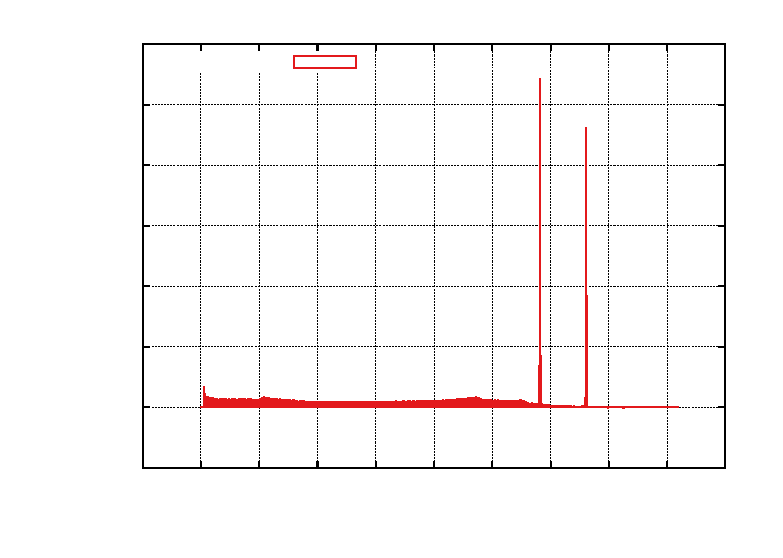
\includegraphics{./plots/halbleiter/cobalt}}%
    \gplfronttext
  \end{picture}%
\endgroup

		}
		\caption{\isotope[60]{Co}-Spektrum mit subtrahiertem Untergrund}
		\label{fig:cobalt_ohne_untergrund}
	\end{subfigure}
	\caption{Subtraktion des gemessenen Untergrundes von dem \isotope[60]{Co}-Spektrum. Die Spektren wurden mit einer Messdauer von $t = \SI{720}{\second}$ aufgenommen. Die Korrektur ist hauptsächlich in den Kanälen $< 1000$ zu erkennen.}
	\label{fig:abzug_untergrund}
\end{figure}
Im Folgenden werden (sofern nicht anders angegeben) alle Spektren gemäß dieser Überlegungen korrigiert, weshalb die korrigierten Ereignisanzahlen ab sofort mit $N$ bezeichnet werden.
Für die Bestimmung der absoluten Peakeffizienz in Abschnitt \ref{sec:absolute_peakeffizienz_szinti} ist der Abstand der radioaktiven Probe vom Detektor nötig, welcher in Tabelle \ref{tab:abstand_szinti} aufgetragen wurde.
\begin{table}[h]
	\centering
	\begin{tabular}{lSS}
\toprule
Isotop & {$d / \si{cm}$} & {$\Delta d / \si{cm}$} \\ \midrule
\isotope[60]{Co} & 2.3 & 0.2 \\
\isotope[137]{Cs} & 17.8 & 0.2 \\
\isotope[152]{Eu} & 24.0 & 0.2 \\ \bottomrule
\end{tabular}
	\caption{Abstände $d$ der Proben vom Szintillationsdetektors}
	\label{tab:abstand_szinti}
\end{table}


\subsubsection{Energiekalibrierung}
\label{sec:kalibrierung_szinti}
Da die Spektren mit einem Vielkanalanalysator aufgenommen werden, kann aus den Daten zunächst keine Energieinformation gewonnen werden.
Dazu ist eine Energiekalibrierung nötig, die mit Hilfe bekannter Linien in den jeweiligen Gamma-Spektren durchgeführt wird.
An gut getrennte Linien wurde dazu eine Gaußfunktion der Form
\begin{align}
\mathcal{G}(n) &= A \cdot \exp\left( - \frac{(n - \mu)^2}{2 \sigma^2}\right) \qquad\text{($n$: Kanalnummer),}
\label{eq:gaussfithypothese}
\end{align}
im Fall nah beieinander liegender Linien eine Summe von solchen Gaußfunktionen angepasst.
Weiterhin wurde in der Anpassungshypothese ein Untergrund $u(n)$ berücksichtigt, der je nach Peak auf Basis der Daten entweder konstant oder linear angenommen wurde.
Zur Verdeutlichung wurde die Anpassung für Cobalt in Abbildung \ref{fig:fit_cobalt} beispielhaft für das Vorgehen dargestellt.
\begin{figure}[ht]
	\centering
	\resizebox{0.85\textwidth}{!}{
	% GNUPLOT: LaTeX picture with Postscript
\begingroup
  \makeatletter
  \providecommand\color[2][]{%
    \GenericError{(gnuplot) \space\space\space\@spaces}{%
      Package color not loaded in conjunction with
      terminal option `colourtext'%
    }{See the gnuplot documentation for explanation.%
    }{Either use 'blacktext' in gnuplot or load the package
      color.sty in LaTeX.}%
    \renewcommand\color[2][]{}%
  }%
  \providecommand\includegraphics[2][]{%
    \GenericError{(gnuplot) \space\space\space\@spaces}{%
      Package graphicx or graphics not loaded%
    }{See the gnuplot documentation for explanation.%
    }{The gnuplot epslatex terminal needs graphicx.sty or graphics.sty.}%
    \renewcommand\includegraphics[2][]{}%
  }%
  \providecommand\rotatebox[2]{#2}%
  \@ifundefined{ifGPcolor}{%
    \newif\ifGPcolor
    \GPcolortrue
  }{}%
  \@ifundefined{ifGPblacktext}{%
    \newif\ifGPblacktext
    \GPblacktexttrue
  }{}%
  % define a \g@addto@macro without @ in the name:
  \let\gplgaddtomacro\g@addto@macro
  % define empty templates for all commands taking text:
  \gdef\gplbacktext{}%
  \gdef\gplfronttext{}%
  \makeatother
  \ifGPblacktext
    % no textcolor at all
    \def\colorrgb#1{}%
    \def\colorgray#1{}%
  \else
    % gray or color?
    \ifGPcolor
      \def\colorrgb#1{\color[rgb]{#1}}%
      \def\colorgray#1{\color[gray]{#1}}%
      \expandafter\def\csname LTw\endcsname{\color{white}}%
      \expandafter\def\csname LTb\endcsname{\color{black}}%
      \expandafter\def\csname LTa\endcsname{\color{black}}%
      \expandafter\def\csname LT0\endcsname{\color[rgb]{1,0,0}}%
      \expandafter\def\csname LT1\endcsname{\color[rgb]{0,1,0}}%
      \expandafter\def\csname LT2\endcsname{\color[rgb]{0,0,1}}%
      \expandafter\def\csname LT3\endcsname{\color[rgb]{1,0,1}}%
      \expandafter\def\csname LT4\endcsname{\color[rgb]{0,1,1}}%
      \expandafter\def\csname LT5\endcsname{\color[rgb]{1,1,0}}%
      \expandafter\def\csname LT6\endcsname{\color[rgb]{0,0,0}}%
      \expandafter\def\csname LT7\endcsname{\color[rgb]{1,0.3,0}}%
      \expandafter\def\csname LT8\endcsname{\color[rgb]{0.5,0.5,0.5}}%
    \else
      % gray
      \def\colorrgb#1{\color{black}}%
      \def\colorgray#1{\color[gray]{#1}}%
      \expandafter\def\csname LTw\endcsname{\color{white}}%
      \expandafter\def\csname LTb\endcsname{\color{black}}%
      \expandafter\def\csname LTa\endcsname{\color{black}}%
      \expandafter\def\csname LT0\endcsname{\color{black}}%
      \expandafter\def\csname LT1\endcsname{\color{black}}%
      \expandafter\def\csname LT2\endcsname{\color{black}}%
      \expandafter\def\csname LT3\endcsname{\color{black}}%
      \expandafter\def\csname LT4\endcsname{\color{black}}%
      \expandafter\def\csname LT5\endcsname{\color{black}}%
      \expandafter\def\csname LT6\endcsname{\color{black}}%
      \expandafter\def\csname LT7\endcsname{\color{black}}%
      \expandafter\def\csname LT8\endcsname{\color{black}}%
    \fi
  \fi
    \setlength{\unitlength}{0.0500bp}%
    \ifx\gptboxheight\undefined%
      \newlength{\gptboxheight}%
      \newlength{\gptboxwidth}%
      \newsavebox{\gptboxtext}%
    \fi%
    \setlength{\fboxrule}{0.5pt}%
    \setlength{\fboxsep}{1pt}%
\begin{picture}(7488.00,5040.00)%
    \gplgaddtomacro\gplbacktext{%
      \csname LTb\endcsname%
      \put(946,704){\makebox(0,0)[r]{\strut{}$0$}}%
      \csname LTb\endcsname%
      \put(946,1383){\makebox(0,0)[r]{\strut{}$200$}}%
      \csname LTb\endcsname%
      \put(946,2061){\makebox(0,0)[r]{\strut{}$400$}}%
      \csname LTb\endcsname%
      \put(946,2740){\makebox(0,0)[r]{\strut{}$600$}}%
      \csname LTb\endcsname%
      \put(946,3418){\makebox(0,0)[r]{\strut{}$800$}}%
      \csname LTb\endcsname%
      \put(946,4097){\makebox(0,0)[r]{\strut{}$1000$}}%
      \csname LTb\endcsname%
      \put(946,4775){\makebox(0,0)[r]{\strut{}$1200$}}%
      \csname LTb\endcsname%
      \put(1078,484){\makebox(0,0){\strut{}$6000$}}%
      \csname LTb\endcsname%
      \put(1937,484){\makebox(0,0){\strut{}$6100$}}%
      \csname LTb\endcsname%
      \put(2796,484){\makebox(0,0){\strut{}$6200$}}%
      \csname LTb\endcsname%
      \put(3655,484){\makebox(0,0){\strut{}$6300$}}%
      \csname LTb\endcsname%
      \put(4514,484){\makebox(0,0){\strut{}$6400$}}%
      \csname LTb\endcsname%
      \put(5373,484){\makebox(0,0){\strut{}$6500$}}%
      \csname LTb\endcsname%
      \put(6232,484){\makebox(0,0){\strut{}$6600$}}%
      \csname LTb\endcsname%
      \put(7091,484){\makebox(0,0){\strut{}$6700$}}%
    }%
    \gplgaddtomacro\gplfronttext{%
      \csname LTb\endcsname%
      \put(176,2739){\rotatebox{-270}{\makebox(0,0){\strut{}Ereignisse $N$}}}%
      \put(4084,154){\makebox(0,0){\strut{}Kanalnummer $n$}}%
      \put(4084,4665){\makebox(0,0){\strut{}}}%
      \csname LTb\endcsname%
      \put(6104,4602){\makebox(0,0)[r]{\strut{}Messwerte}}%
      \csname LTb\endcsname%
      \put(6104,4382){\makebox(0,0)[r]{\strut{}$\Sigma$}}%
      \csname LTb\endcsname%
      \put(6104,4162){\makebox(0,0)[r]{\strut{}$\mathcal{G}_1$}}%
      \csname LTb\endcsname%
      \put(6104,3942){\makebox(0,0)[r]{\strut{}$\mathcal{G}_2$}}%
      \csname LTb\endcsname%
      \put(6104,3722){\makebox(0,0)[r]{\strut{}$u$}}%
    }%
    \gplbacktext
    \put(0,0){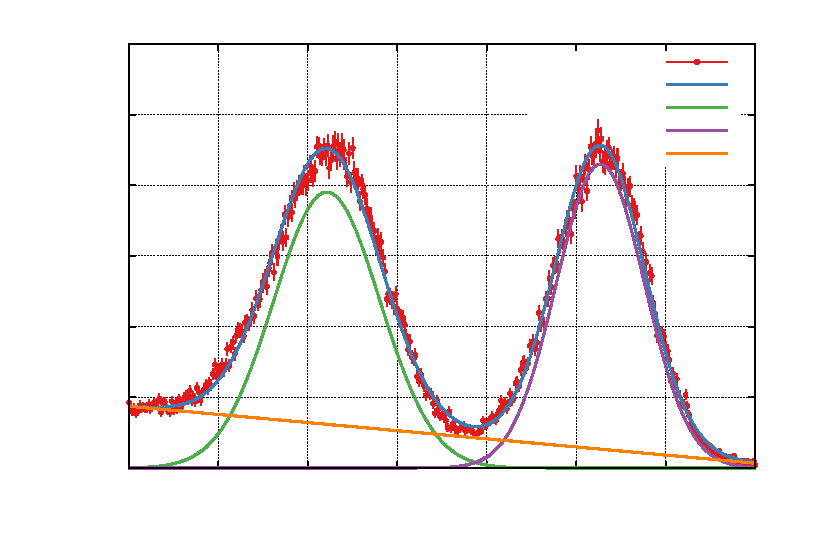
\includegraphics{./plots/szintillator/energiekalibrierung/cobalt_darstellung}}%
    \gplfronttext
  \end{picture}%
\endgroup

	}
	\caption{Anpassung für die Linien im Gammaspektrum von Cobalt}
	\label{fig:fit_cobalt}
\end{figure}
In Tabelle \ref{tab:kalibrierungslinien_szinti} sind die Ergebnisse der Anpassung eingetragen, wobei für die Kalibrierung zunächst nur der Linienschwerpunkt $n$ und die Gammaenergie $E_\gamma$ relevant sind.
Den Schwerpunkten der Gaußfunktionen wurden dabei unter Benutzung der Termschemata und Tabelle in \cite{anleitung} die jeweiligen Gammaenergien zugeordnet.
\begin{table}[ht]
	\centering
	\begin{tabular}{lSSS}
\toprule
Element & {Linienschwerpunkt $n$} & {$\Delta n$} & {Gammaenergie $E_{\gamma}$ / \si{\kilo\electronvolt}} \\ \midrule
Co      & 6216.88               & 0.58       & 1173.24      \\
Co      & 6523.72               & 0.28       & 1332.50      \\
Cs      & 3844.05               & 0.59       & 661.66       \\
Eu      & 728.25                & 0.53       & 121.78       \\
Eu      & 1421.21               & 2.37       & 244.70       \\
Eu      & 1997.48               & 0.50       & 344.28       \\
Eu      & 4511.39               & 2.16       & 778.90       \\
Eu      & 5535.31               & 1.70       & 964.13       \\
Eu      & 6030.90               & 0.89       & 1112.12      \\
Eu      & 6630.78               & 0.96       & 1408.01      \\ \bottomrule
\end{tabular}
	\caption{Anpassungsergebnisse zur Energiekalibrierung für den NaI(Tl) Szintillationsdetektor}
	\label{tab:kalibrierungslinien_szinti}
\end{table}
Der Zusammenhang zwischen Kanalnummer und Energie wird als linear betrachtet, so dass eine Anpassung an eine Gerade mit Steigung $m$ und Achsenabschnitt $b$ erfolgt.
Für Kanalnummern über \num{6000} weichen die gefundenen Messwerte deutlich von dem linearen Verlauf der Kanalnummern kleiner als \num{6000} ab, so dass hier nicht die gleiche Kalibrierung verwendet werden kann.
Für diesen Bereich wurde auf Grundlage der dort liegenden \num{4} Datenpunkte eine zweite Kalibrierung (mit gleicher Anpassungshypothese) durchgeführt, so dass im weiteren Verlauf je nach betrachtetem Kanalbereich die dort gültige Kalibrierung gewählt werden muss. 
Die Daten und durchgeführte Anpassung sind in Abbildung \ref{fig:kalibrierung_szinti} zu sehen.
\begin{figure}[ht]
	\centering
	\begin{tabular}{lSSS}
\toprule
Element & {Linienschwerpunkt $n$} & {$\Delta n$} & {Gammaenergie $E_{\gamma}$ / \si{\kilo\electronvolt}} \\ \midrule
Co      & 6216.88               & 0.58       & 1173.24      \\
Co      & 6523.72               & 0.28       & 1332.50      \\
Cs      & 3844.05               & 0.59       & 661.66       \\
Eu      & 728.25                & 0.53       & 121.78       \\
Eu      & 1421.21               & 2.37       & 244.70       \\
Eu      & 1997.48               & 0.50       & 344.28       \\
Eu      & 4511.39               & 2.16       & 778.90       \\
Eu      & 5535.31               & 1.70       & 964.13       \\
Eu      & 6030.90               & 0.89       & 1112.12      \\
Eu      & 6630.78               & 0.96       & 1408.01      \\ \bottomrule
\end{tabular}
	\caption{Energiekalibrierung des NaI(Tl) Detektors. Die Fehler sind zu klein, um gesehen werden zu können.}
	\label{fig:kalibrierung_szinti}
\end{figure}
Die Anpassungsergebnisse lauten:
\begin{align}
	m = 
	\begin{cases}
	\SI{0.17441+-0.00076}{\kilo\electronvolt} & n < 6000 \\
	\SI{0.48976+-0.04034}{\kilo\electronvolt} & n > 6000
	\end{cases}\\
	b = 
	\begin{cases}
	\SI{-5.189+-2.627}{\kilo\electronvolt} & n < 6000 \\
	\SI{-1855.53+-256.50}{\kilo\electronvolt} & n > 6000
	\end{cases}
\end{align}
Da die Anpassungsgerade für den Halbleiterdetektor eine deutlich bessere und durchgehend lineare Übereinstimmung mit den Messwerten zeigt, liegt die Ursache für den beobachteten Verlauf nicht an dem verwendeten Vielkanalanalysator sondern ist im Verstärker zu suchen.

Da im Folgenden oftmals eine Umrechnung von Kanalnummer $n$ auf Gammaenergie $E_\gamma$ erfolgt, soll hier die Vorgehensweise einmalig erklärt werden.
Die Kalibrierung bildet den linearen Zusammenhang zwischen $E_\gamma$ und $n$:
\begin{align}
	E_\gamma = m \cdot n + b
\end{align}
da oftmals die Kanalnummer mit einem Fehler behaftet ist (z.B. bei den Linienschwerpunkten) muss dies bei der Fehlerfortpflanzung:
\begin{align}
	\Delta E_\gamma = \sqrt{n^2 \cdot \Delta m^2 + m^2 \cdot \Delta n^2 + \Delta b^2}
\end{align}
berücksichtigt werden.

\subsubsection{Halbwertsbreiten der Linien}
Zur Bestimmung der Halbwertsbreiten kann die Anpassung der Gaußfunktionen an die jeweilige Linie verwendet werden, welche bereits bei der Energiekalibrierung in Abschnitt \ref{sec:kalibrierung_szinti} durchgeführt werden.
Dazu kann die Standardabweichung $\sigma$ der Gaußfunktion in die volle Halbwertsbreite (FWHM: \textit{full width at half maximum}) durch
\begin{align}
	\text{FWHM} = 2 \, \sqrt{2\ln(2)} \cdot \sigma
\end{align}
umgerechnet werden.
Der Fehler wird dementsprechend durch
\begin{align}
	\Delta \text{FWHM} = 2 \, \sqrt{2\ln(2)} \cdot \Delta \sigma
\end{align}
fortgepflanzt.
Mit den Anpassungsergebnissen aus Tabelle \ref{tab:kalibrierungslinien_szinti} kann dementsprechend die Halbwertsbreite in Einheiten der Kanalnummer berechnet werden.
Diese kann mithilfe der Energiekalibrierung in Abschnitt \ref{sec:kalibrierung_szinti} in Einheiten der Energie umgerechnet werden, wobei die Fehler erneut durch Gauß'sche Fehlerfortpflanzung ermittelt werden.
Konkret erfolgt die Umrechnung durch Multiplikation der Halbwertsbreite in Einheiten der Kanalnummer mit der Steigung der Kalibrierungsgeraden, da die volle Halbwertsbreite eine Differenzgröße ist und dadurch konstanter Versatz keinen Einfluss nimmt.
\begin{table}[ht]
	\centering
	\begin{tabular}{lSSSSS}
\toprule
Isotop & {Gammaenergie} & {FWHM} & {$\Delta \text{FWHM}$} & {FWHM} & {$\Delta \text{FWHM}$}\\
       & {$E_\gamma$ / \si{keV}}             & \multicolumn{2}{c}{Kanäle} & \multicolumn{2}{c}{\si{keV}} \\
\midrule
Co            & 1173.237 & 139.8  & 0.9        & 68.5   & 5.7 \\
Co            & 1332.501 & 116.2  & 0.6        & 56.9   & 4.7 \\
Cs            & 661.660  & 269.1  & 1.3        & 46.9   & 0.3 \\
Eu            & 121.783  & 72.8   & 0.6        & 12.7   & 0.2 \\
Eu            & 244.699  & 106.0  & 6.2        & 18.5   & 1.1 \\
Eu            & 344.281  & 185.7  & 2.4        & 32.4   & 0.5 \\
Eu            & 778.903  & 260.9  & 6.6        & 45.5   & 1.2 \\
Eu            & 964.131  & 235.4  & 5.9        & 41.1   & 1.1 \\
Eu            & 1112.116 & 186.0  & 3.5        & 91.1   & 7.7 \\
Eu            & 1408.011 & 109.3  & 1.8        & 53.5   & 4.5 \\
\bottomrule
\end{tabular}
	\caption{Volle Halbwertsbreiten der zur Kalibration verwendeten Linien in den Spektren von \isotope[60]{Co}, \isotope[137]{Cs} und \isotope[152]{Eu}.}
	\label{tab:fwhm_szinti}
\end{table}
Die berechneten Breiten wurden in Tabelle \ref{tab:fwhm_szinti} zusammengetragen.
Leider führt die Nichtlinearität des Verstärkers bei der stückweisen Energiekalibrierung zu einer Verfälschung der Halbwertsbreite der Linien mit einer Energie größer als \SI{1000}{\kilo\electronvolt}, weshalb diese nur als Größenordnungen betrachtet werden sollten.
Die Halbwertsbreiten für Linien geringerer Energie sollten hingegen akkurat wiedergegeben werden.
Betrachtet man nur Linien geringerer Energie so zeigt sich die erwartete Zunahme der Linienbreite mit steigender Energie, welche in dem statistischen Prozess der Photonenemission im Szintillator begründet liegt.

\subsubsection{Peak-to-Total Verhältnis}
Zur Bestimmung des Peak-to-Total Verhältnisses muss die Gesamtzahl aller Ereignisse $N_\mathrm{tot.}$ in den Spektren bestimmt werden.
Diese erhält man durch Subtraktion der Gesamtzahl der Ereignisse der Untergrundmessung $N_\mathrm{Untergrund}$ von der untergrundbehafteten Ereigniszahl des Spektrums $N_0$:
\begin{align}
	N_\mathrm{tot.} = N_\mathrm{0} - N_\mathrm{Untergrund}
\end{align}
dabei wird auf die Anzahlen der Fehler gemäß der Poisson-Verteilung angenommen.
Neben der Gesamtzahl wird sowohl die Anzahl der Ereignisse in den Photopeaks als auch im Rückstreupeak benötigt.
Diese können direkt durch Integration über die Anpassung der Gaußfunktion berechnet werden:
\begin{align}
\int_{-\infty}^{\infty} \mathcal{G}(n) \, \mathrm{d}n = \sqrt{2 \pi} \sigma A
\label{eq:integral_peak}
\end{align}
Die Anpassungsparameter für die Photopeaks können direkt aus Abschnitt \ref{sec:kalibrierung_szinti} übernommen werden.
Analog zur Kalibrierung wird eine Anpassung an die Rückstreupeaks von \isotope[60]{Co} und \isotope[137]{Cs} durchgeführt.
Exemplarisch dafür wurde die Anpassung an den Rückstreupeak von \isotope[137]{Cs} in Abbildung \ref{fig:fit_rueck_szinti} durchgeführt.
\begin{figure}[h]
	\centering
	% GNUPLOT: LaTeX picture with Postscript
\begingroup
  \makeatletter
  \providecommand\color[2][]{%
    \GenericError{(gnuplot) \space\space\space\@spaces}{%
      Package color not loaded in conjunction with
      terminal option `colourtext'%
    }{See the gnuplot documentation for explanation.%
    }{Either use 'blacktext' in gnuplot or load the package
      color.sty in LaTeX.}%
    \renewcommand\color[2][]{}%
  }%
  \providecommand\includegraphics[2][]{%
    \GenericError{(gnuplot) \space\space\space\@spaces}{%
      Package graphicx or graphics not loaded%
    }{See the gnuplot documentation for explanation.%
    }{The gnuplot epslatex terminal needs graphicx.sty or graphics.sty.}%
    \renewcommand\includegraphics[2][]{}%
  }%
  \providecommand\rotatebox[2]{#2}%
  \@ifundefined{ifGPcolor}{%
    \newif\ifGPcolor
    \GPcolortrue
  }{}%
  \@ifundefined{ifGPblacktext}{%
    \newif\ifGPblacktext
    \GPblacktexttrue
  }{}%
  % define a \g@addto@macro without @ in the name:
  \let\gplgaddtomacro\g@addto@macro
  % define empty templates for all commands taking text:
  \gdef\gplbacktext{}%
  \gdef\gplfronttext{}%
  \makeatother
  \ifGPblacktext
    % no textcolor at all
    \def\colorrgb#1{}%
    \def\colorgray#1{}%
  \else
    % gray or color?
    \ifGPcolor
      \def\colorrgb#1{\color[rgb]{#1}}%
      \def\colorgray#1{\color[gray]{#1}}%
      \expandafter\def\csname LTw\endcsname{\color{white}}%
      \expandafter\def\csname LTb\endcsname{\color{black}}%
      \expandafter\def\csname LTa\endcsname{\color{black}}%
      \expandafter\def\csname LT0\endcsname{\color[rgb]{1,0,0}}%
      \expandafter\def\csname LT1\endcsname{\color[rgb]{0,1,0}}%
      \expandafter\def\csname LT2\endcsname{\color[rgb]{0,0,1}}%
      \expandafter\def\csname LT3\endcsname{\color[rgb]{1,0,1}}%
      \expandafter\def\csname LT4\endcsname{\color[rgb]{0,1,1}}%
      \expandafter\def\csname LT5\endcsname{\color[rgb]{1,1,0}}%
      \expandafter\def\csname LT6\endcsname{\color[rgb]{0,0,0}}%
      \expandafter\def\csname LT7\endcsname{\color[rgb]{1,0.3,0}}%
      \expandafter\def\csname LT8\endcsname{\color[rgb]{0.5,0.5,0.5}}%
    \else
      % gray
      \def\colorrgb#1{\color{black}}%
      \def\colorgray#1{\color[gray]{#1}}%
      \expandafter\def\csname LTw\endcsname{\color{white}}%
      \expandafter\def\csname LTb\endcsname{\color{black}}%
      \expandafter\def\csname LTa\endcsname{\color{black}}%
      \expandafter\def\csname LT0\endcsname{\color{black}}%
      \expandafter\def\csname LT1\endcsname{\color{black}}%
      \expandafter\def\csname LT2\endcsname{\color{black}}%
      \expandafter\def\csname LT3\endcsname{\color{black}}%
      \expandafter\def\csname LT4\endcsname{\color{black}}%
      \expandafter\def\csname LT5\endcsname{\color{black}}%
      \expandafter\def\csname LT6\endcsname{\color{black}}%
      \expandafter\def\csname LT7\endcsname{\color{black}}%
      \expandafter\def\csname LT8\endcsname{\color{black}}%
    \fi
  \fi
    \setlength{\unitlength}{0.0500bp}%
    \ifx\gptboxheight\undefined%
      \newlength{\gptboxheight}%
      \newlength{\gptboxwidth}%
      \newsavebox{\gptboxtext}%
    \fi%
    \setlength{\fboxrule}{0.5pt}%
    \setlength{\fboxsep}{1pt}%
\begin{picture}(7200.00,5040.00)%
    \gplgaddtomacro\gplbacktext{%
      \csname LTb\endcsname%
      \put(946,704){\makebox(0,0)[r]{\strut{}$0$}}%
      \csname LTb\endcsname%
      \put(946,1286){\makebox(0,0)[r]{\strut{}$200$}}%
      \csname LTb\endcsname%
      \put(946,1867){\makebox(0,0)[r]{\strut{}$400$}}%
      \csname LTb\endcsname%
      \put(946,2449){\makebox(0,0)[r]{\strut{}$600$}}%
      \csname LTb\endcsname%
      \put(946,3030){\makebox(0,0)[r]{\strut{}$800$}}%
      \csname LTb\endcsname%
      \put(946,3612){\makebox(0,0)[r]{\strut{}$1000$}}%
      \csname LTb\endcsname%
      \put(946,4193){\makebox(0,0)[r]{\strut{}$1200$}}%
      \csname LTb\endcsname%
      \put(946,4775){\makebox(0,0)[r]{\strut{}$1400$}}%
      \csname LTb\endcsname%
      \put(1078,484){\makebox(0,0){\strut{}$0$}}%
      \csname LTb\endcsname%
      \put(2223,484){\makebox(0,0){\strut{}$1000$}}%
      \csname LTb\endcsname%
      \put(3368,484){\makebox(0,0){\strut{}$2000$}}%
      \csname LTb\endcsname%
      \put(4513,484){\makebox(0,0){\strut{}$3000$}}%
      \csname LTb\endcsname%
      \put(5658,484){\makebox(0,0){\strut{}$4000$}}%
      \csname LTb\endcsname%
      \put(6803,484){\makebox(0,0){\strut{}$5000$}}%
    }%
    \gplgaddtomacro\gplfronttext{%
      \csname LTb\endcsname%
      \put(176,2739){\rotatebox{-270}{\makebox(0,0){\strut{}Ereignisse $N$}}}%
      \put(3940,154){\makebox(0,0){\strut{}Kanal $n$}}%
      \csname LTb\endcsname%
      \put(5816,4602){\makebox(0,0)[r]{\strut{}Messwerte}}%
    }%
    \gplbacktext
    \put(0,0){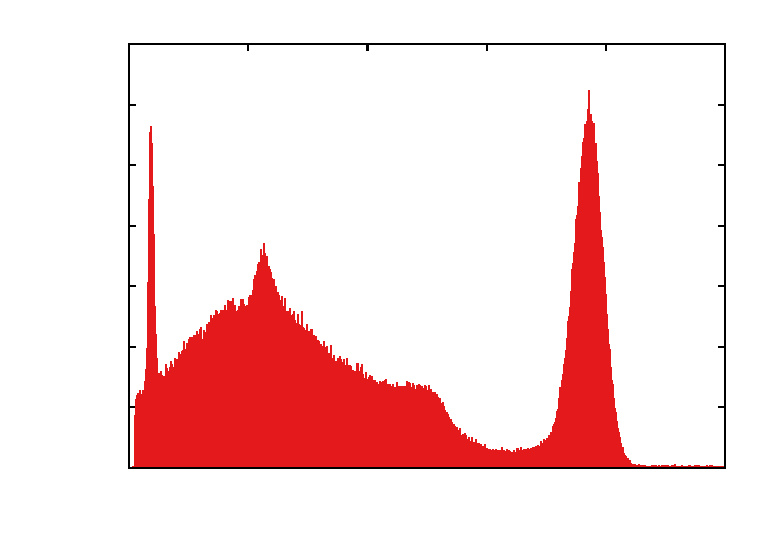
\includegraphics{./plots/szintillator/caesium}}%
    \gplfronttext
  \end{picture}%
\endgroup

	\caption{Anpassung einer Gaußfunktion an den Rückstreupeak von \isotope[137]{Cs}}
	\label{fig:fit_rueck_szinti}
\end{figure}
Die resultierenden Anpassungsparameter wurden in Tabelle \ref{tab:fit_rueck_szinti} aufgetragen.
\begin{table}[ht]
	\centering
	\begin{tabular}{lSSSSSS}
\toprule
Isotop & \multicolumn{2}{c}{Amplitude} & \multicolumn{2}{c}{Schwerpunkt} & \multicolumn{2}{c}{Standardabweichung}\\
       & {$A$} & {$\Delta A$} & {$n$} & {$\Delta n$} & {$\sigma$} & {$\Delta \sigma$}\\
\midrule
\isotope[60]{Co}        & 98.0   & 2.3         & 1374.8 & 3.6    & 145.4  & 5.0 \\
\isotope[137]{Cs}        & 179.0  & 3.0         & 1144.3 & 1.6    & 84.2   & 1.8 \\
\bottomrule
\end{tabular}
	\caption{Ergebnisse der Anpassung von Gaußfunktionen an die Rückstreupeaks}
	\label{tab:fit_rueck_szinti}
\end{table}
Zur Bestimmung des Peak-to-Total Verhältnisses der mittleren Energie der beiden Linien von \isotope[60]{Co} muss die Summe der Photopeaks im Spektrum berechnet werden.
Mit den Werten aus Tabelle \ref{tab:kalibrierungslinien_szinti} und Gleichung \eqref{eq:integral_peak} berechnet sich diese zu:
\begin{align*}
	N_\mathrm{Photo.} &= N_\mathrm{Photo.}(E_\gamma = \SI{780.580}{\kilo\electronvolt}) +  N_\mathrm{Photo.}(E_\gamma = \SI{860.086}{\kilo\electronvolt})\\
	&= (\num{116181 +- 972}) + (\num{106402 +- 771})\\
	&= \num{222582 +- 1241}
\end{align*}
Nun kann das Peak-to-Total Verhältnis $P/T$ durch:
\begin{align}
	P/T = \frac{N_\mathrm{Photo.}}{N_\mathrm{tot.} - N_\mathrm{R"uck.}}
\end{align}
berechnet werden.
Dies wurde in Tabelle \ref{tab:ptt_szinti} für die mittlere Energie der beiden Cobalt Linien und der Caesium Linie durchgeführt.
\begin{table}[ht]
	\centering
	\resizebox{\textwidth}{!}{
	\begin{tabular}{lrrrrrrSS}
\toprule
{Isotop} & {$N_\mathrm{tot.}$} & {$\Delta N_\mathrm{tot.}$} & {$N_\mathrm{Photo.}$} & {$\Delta N_\mathrm{Photo.}$} & {$N_\mathrm{R"uck.}$} & {$\Delta N_\mathrm{R"uck.}$} & {$P/T$}   & {$\Delta P/T$} \\
\midrule
\isotope[60]{Co} & 1301431    & 1219   & 222582    & 1241   & 35707         & 1464   & 17.59 \% & 0.12 \% \\
\isotope[137]{Cs} & 1319403    & 1226   & 304462    & 2279   & 37801         & 1012   & 23.76 \% & 0.18 \% \\
\bottomrule
\end{tabular}
	}
	\caption{Peak-to-Total Verhältnis $P/T$ der beiden Isotope \co{} und \cs{} für den Szintillationsdetektor. Aufgetragen ist die totale Anzahl der Ereignisse $N_\mathrm{tot.}$ (ohne Untergrund), die Anzahl der Ereignisse in den Photopeaks $N_\mathrm{Photo.}$ und die Anzahl der Ereignisse im Rückstreupeak $N_\mathrm{R"uck.}$.}
	\label{tab:ptt_szinti}
\end{table}



\subsubsection{Absolute Peakeffizienz}
\label{sec:absolute_peakeffizienz_szinti}
Zur Bestimmung der absoluten Peakeffizienz des Detektors wird die Aktivität der \cs{}-Quelle benötigt. Da in \cite{anleitung} die Aktivität der Quelle $A_0$ im April 1985 gegeben ist, kann mithilfe des Zerfallsgesetzes:
\begin{align}
	A(t) = A_0 \exp\left( - \frac{\ln(2)\, t}{t_{1/2}} \right)
\end{align}
die Aktivität zum Zeitpunkt der Durchführung $t = \SI{30.03 +- 0.05}{a}$ berechnet werden.
Mit der gegebenen Aktivität $A_0 = \SI{25 +- 1}{\micro Ci}$ (der Fehler wurde gemäß der angegebenen signifikanten Stellen abgeschätzt) und der Halbwertszeit von \cs{} $t_{1/2} = \SI{30.17 +- 0.03}{a}$ aus \cite{nist} folgt zum Zeitpunkt der Durchführung:
\begin{align}
	A = \SI{12.5 +- 0.6}{\micro Ci}
\end{align}
Mit dem Abstand der Quelle vom Detektor $d = \SI{17.8 +- 0.2}{cm}$, dem Radius des Detektors $r_\mathrm{NaI(Tl)} = \SI{24 +- 0.5}{mm}$, der Messdauer $T = \SI{720 +- 1}{\second}$ und der Anzahl der Ereignisse im Photopeak des Caesium-Spektrums aus Tabelle \ref{tab:ptt_szinti} folgt für die absolute Peakeffizienz (Gleichung \ref{eq:peakeffizienz}):
\begin{align}
	\mathcal{E}_\mathrm{NaI(Tl)} = \SI{20.1 +- 1.4}{\percent}
\end{align}
dabei wird aufgrund der Komplexität auf Angabe einer ausführlichen Fehlerformel verzichtet.
Anschaulich bedeutet dies, dass etwa jedes fünfte Gammaquant, welches in Richtung des Detektors emittiert wird, in den Photopeak des Spektrums fällt.

\subsection{Germanium Halbleiterdetektor}
Viele der folgenden Aufgaben erfolgen in Analogie zur Auswertung für den NaI(Tl) Szintillationsdetektor, so dass hier nicht alles wiederholt werden soll.
Dies betrifft insbesondere Formeln für die Fehler.

\subsubsection{Detektorsignal des Halbleiterdetektor}
Im Folgenden soll analog zu Abschnitt \ref{sec:detektorsignal_szinti} das Detektorsignal an Vor- und Hauptverstärker des Ge-Halbleiterdetektors bestimmt werden.
Die genannten Größen und ihre Fehler werden in Analogie zum Szintillationsdetektor bestimmt.
Zunächst soll das Signal am Vorverstärker des Halbleiterdetektors in Abbildung \ref{fig:signal_ger_vor} betrachtet werden.
Die Impulsform ist nahezu identisch mit der des Szintillationsdetektors mit der Ausnahme, dass das Signal hier einen positiven Spannungsausschlag mit der Amplitude $\Delta U = \SI{0.29 +-0.01}{\volt}$ (Anstiegszeit $<\SI{1}{\micro\second}$) aufweist.
Auch der exponentielle Abfall mit der Signaldauer $\Delta t = \SI{137 +- 5}{\micro\second}$ (von 10 \% auf 10\%) ist wiederzuerkennen, wobei dieser in dem Fall nicht durch den Zerfall angeregter Zustände zu erklären ist, sondern auf die Ladungssammlung im Halbleiterkristall zurückzuführen ist.
\begin{figure}[h]
	\centering
	\begin{subfigure}[b]{0.7\textwidth}
		\centering
		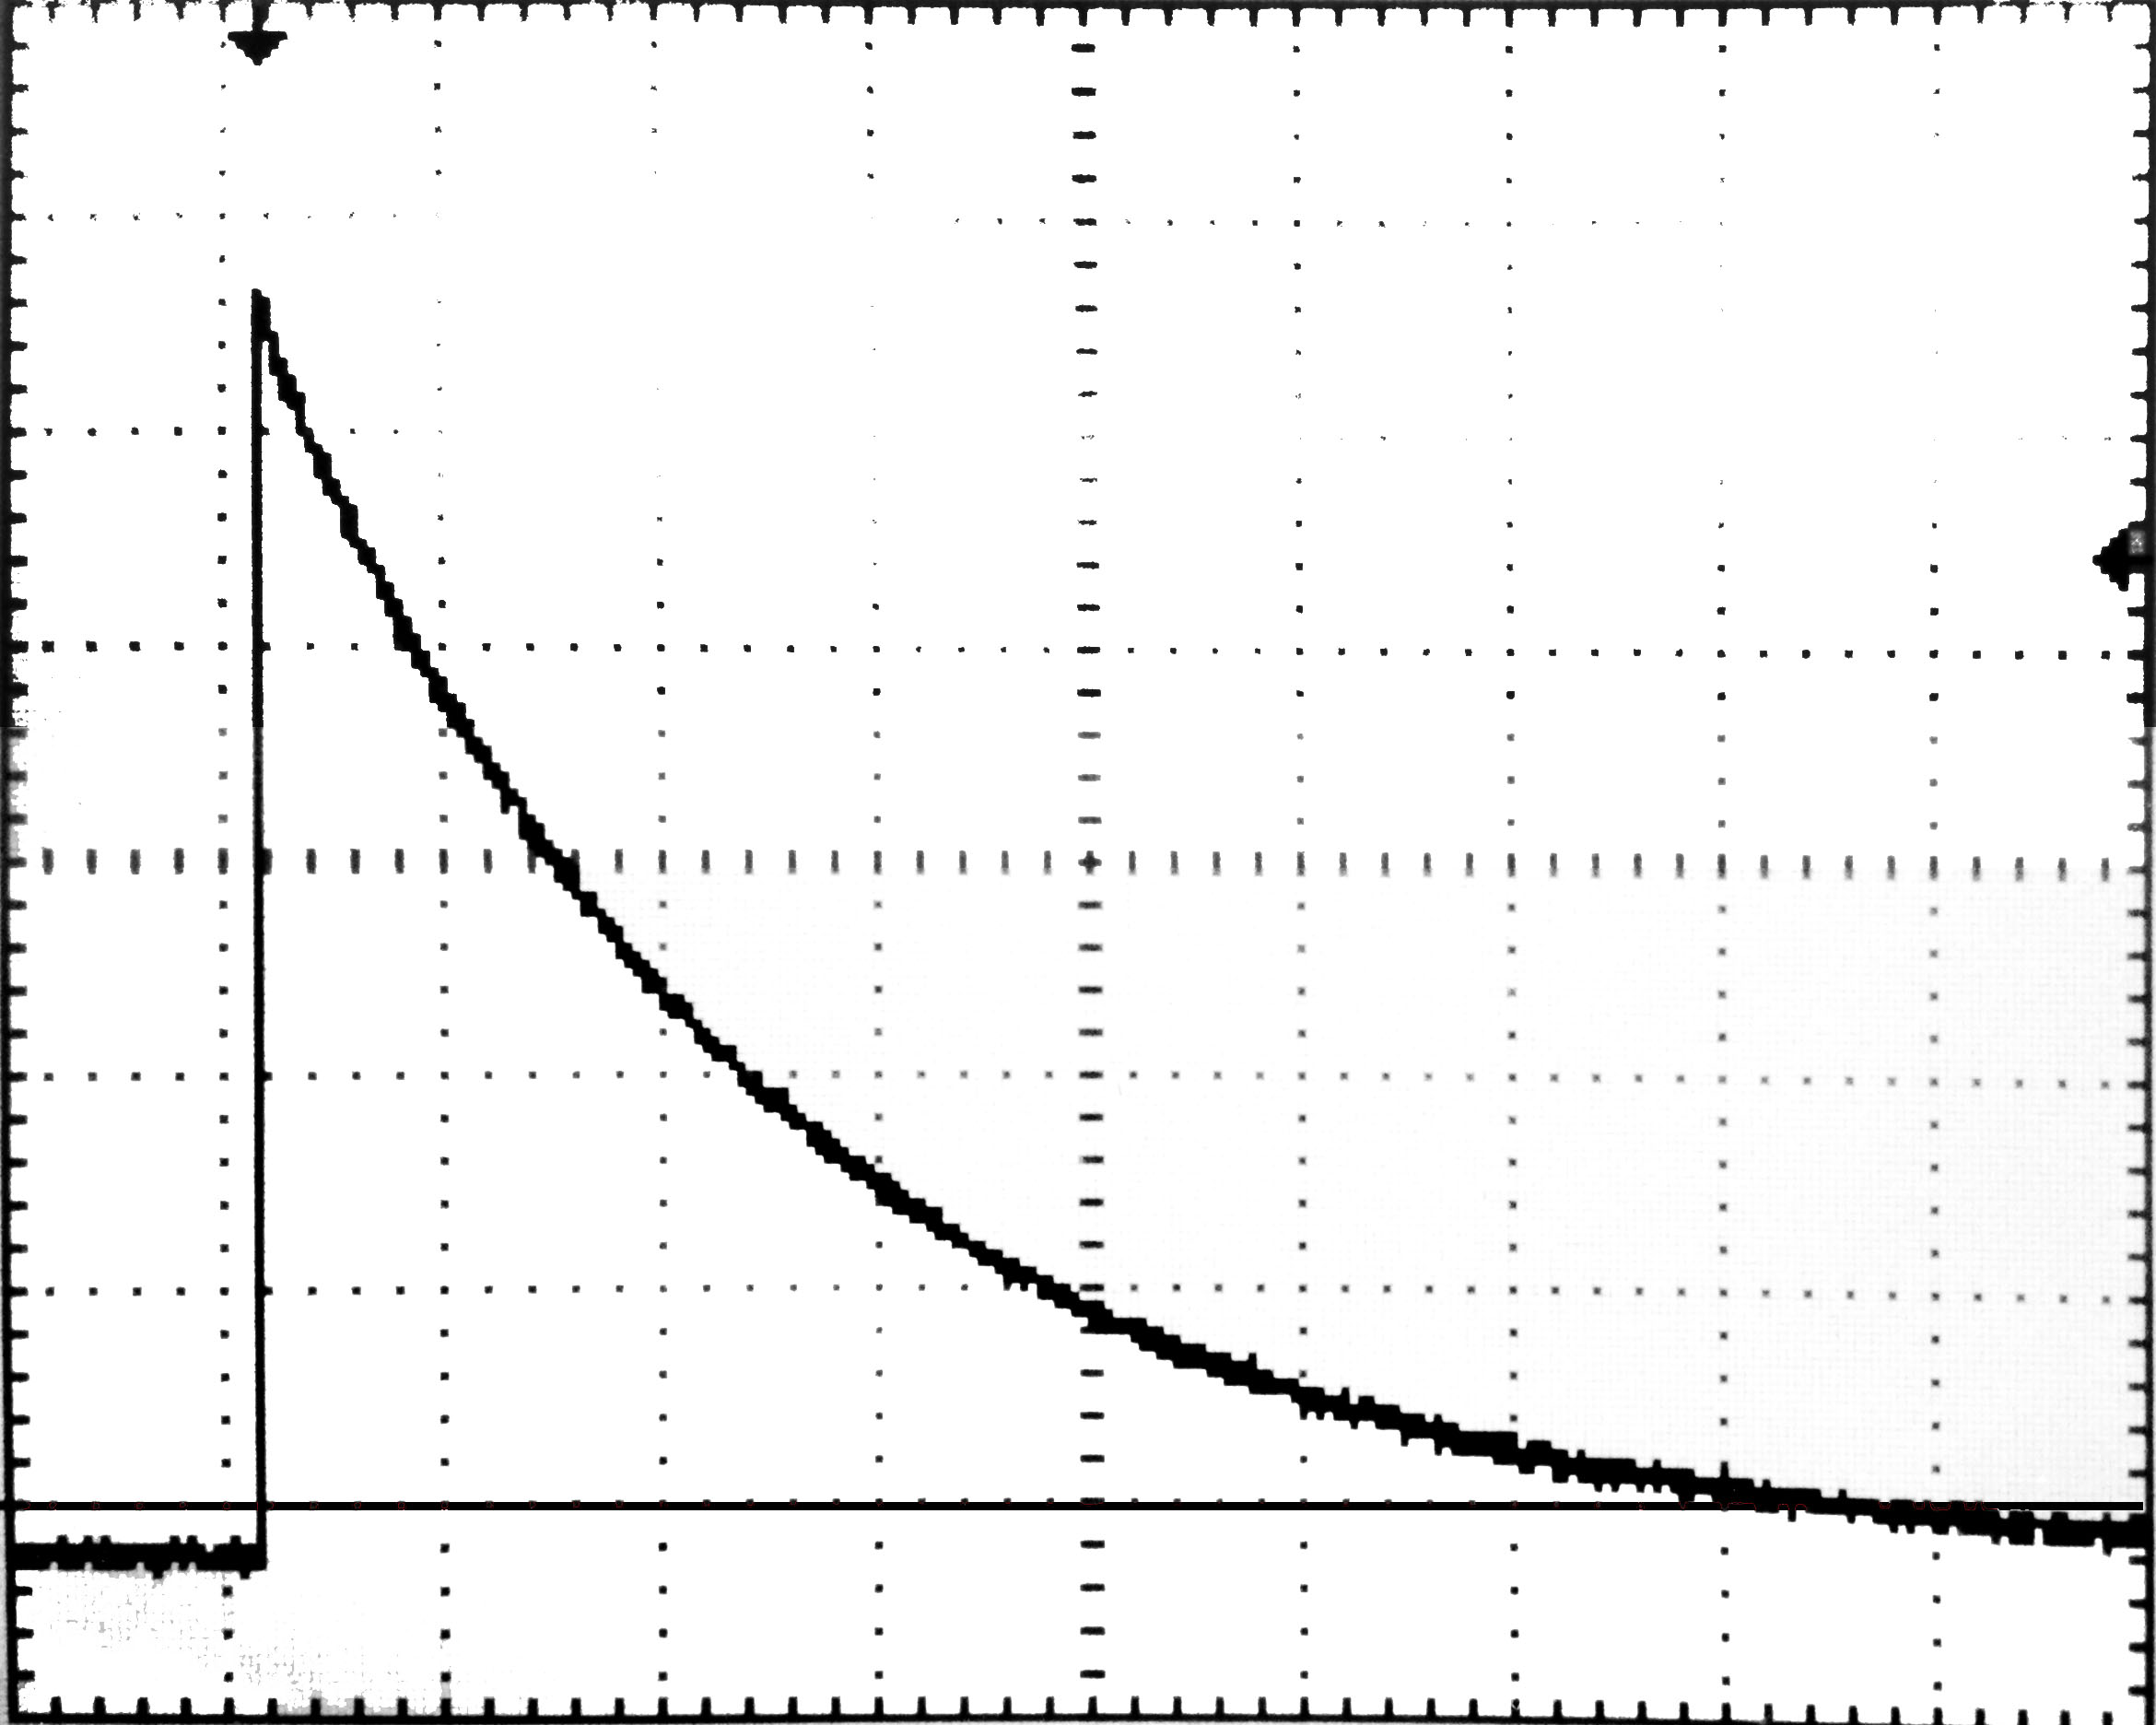
\includegraphics[width=0.7\textwidth]{./figures/signale/vor_ger_abgeschnitten.jpg}
		\caption{Am Ausgang des Vorverstärkers. Die eingestellten Skalenfaktoren am Oszilloskop betragen \SI{50}{\milli\volt\per\division} für die Vertikale und \SI{25}{\micro\second\per\division} in der Horizontalen.}
		\label{fig:signal_ger_vor}
	\end{subfigure}

	\begin{subfigure}[b]{0.7\textwidth}
		\centering
		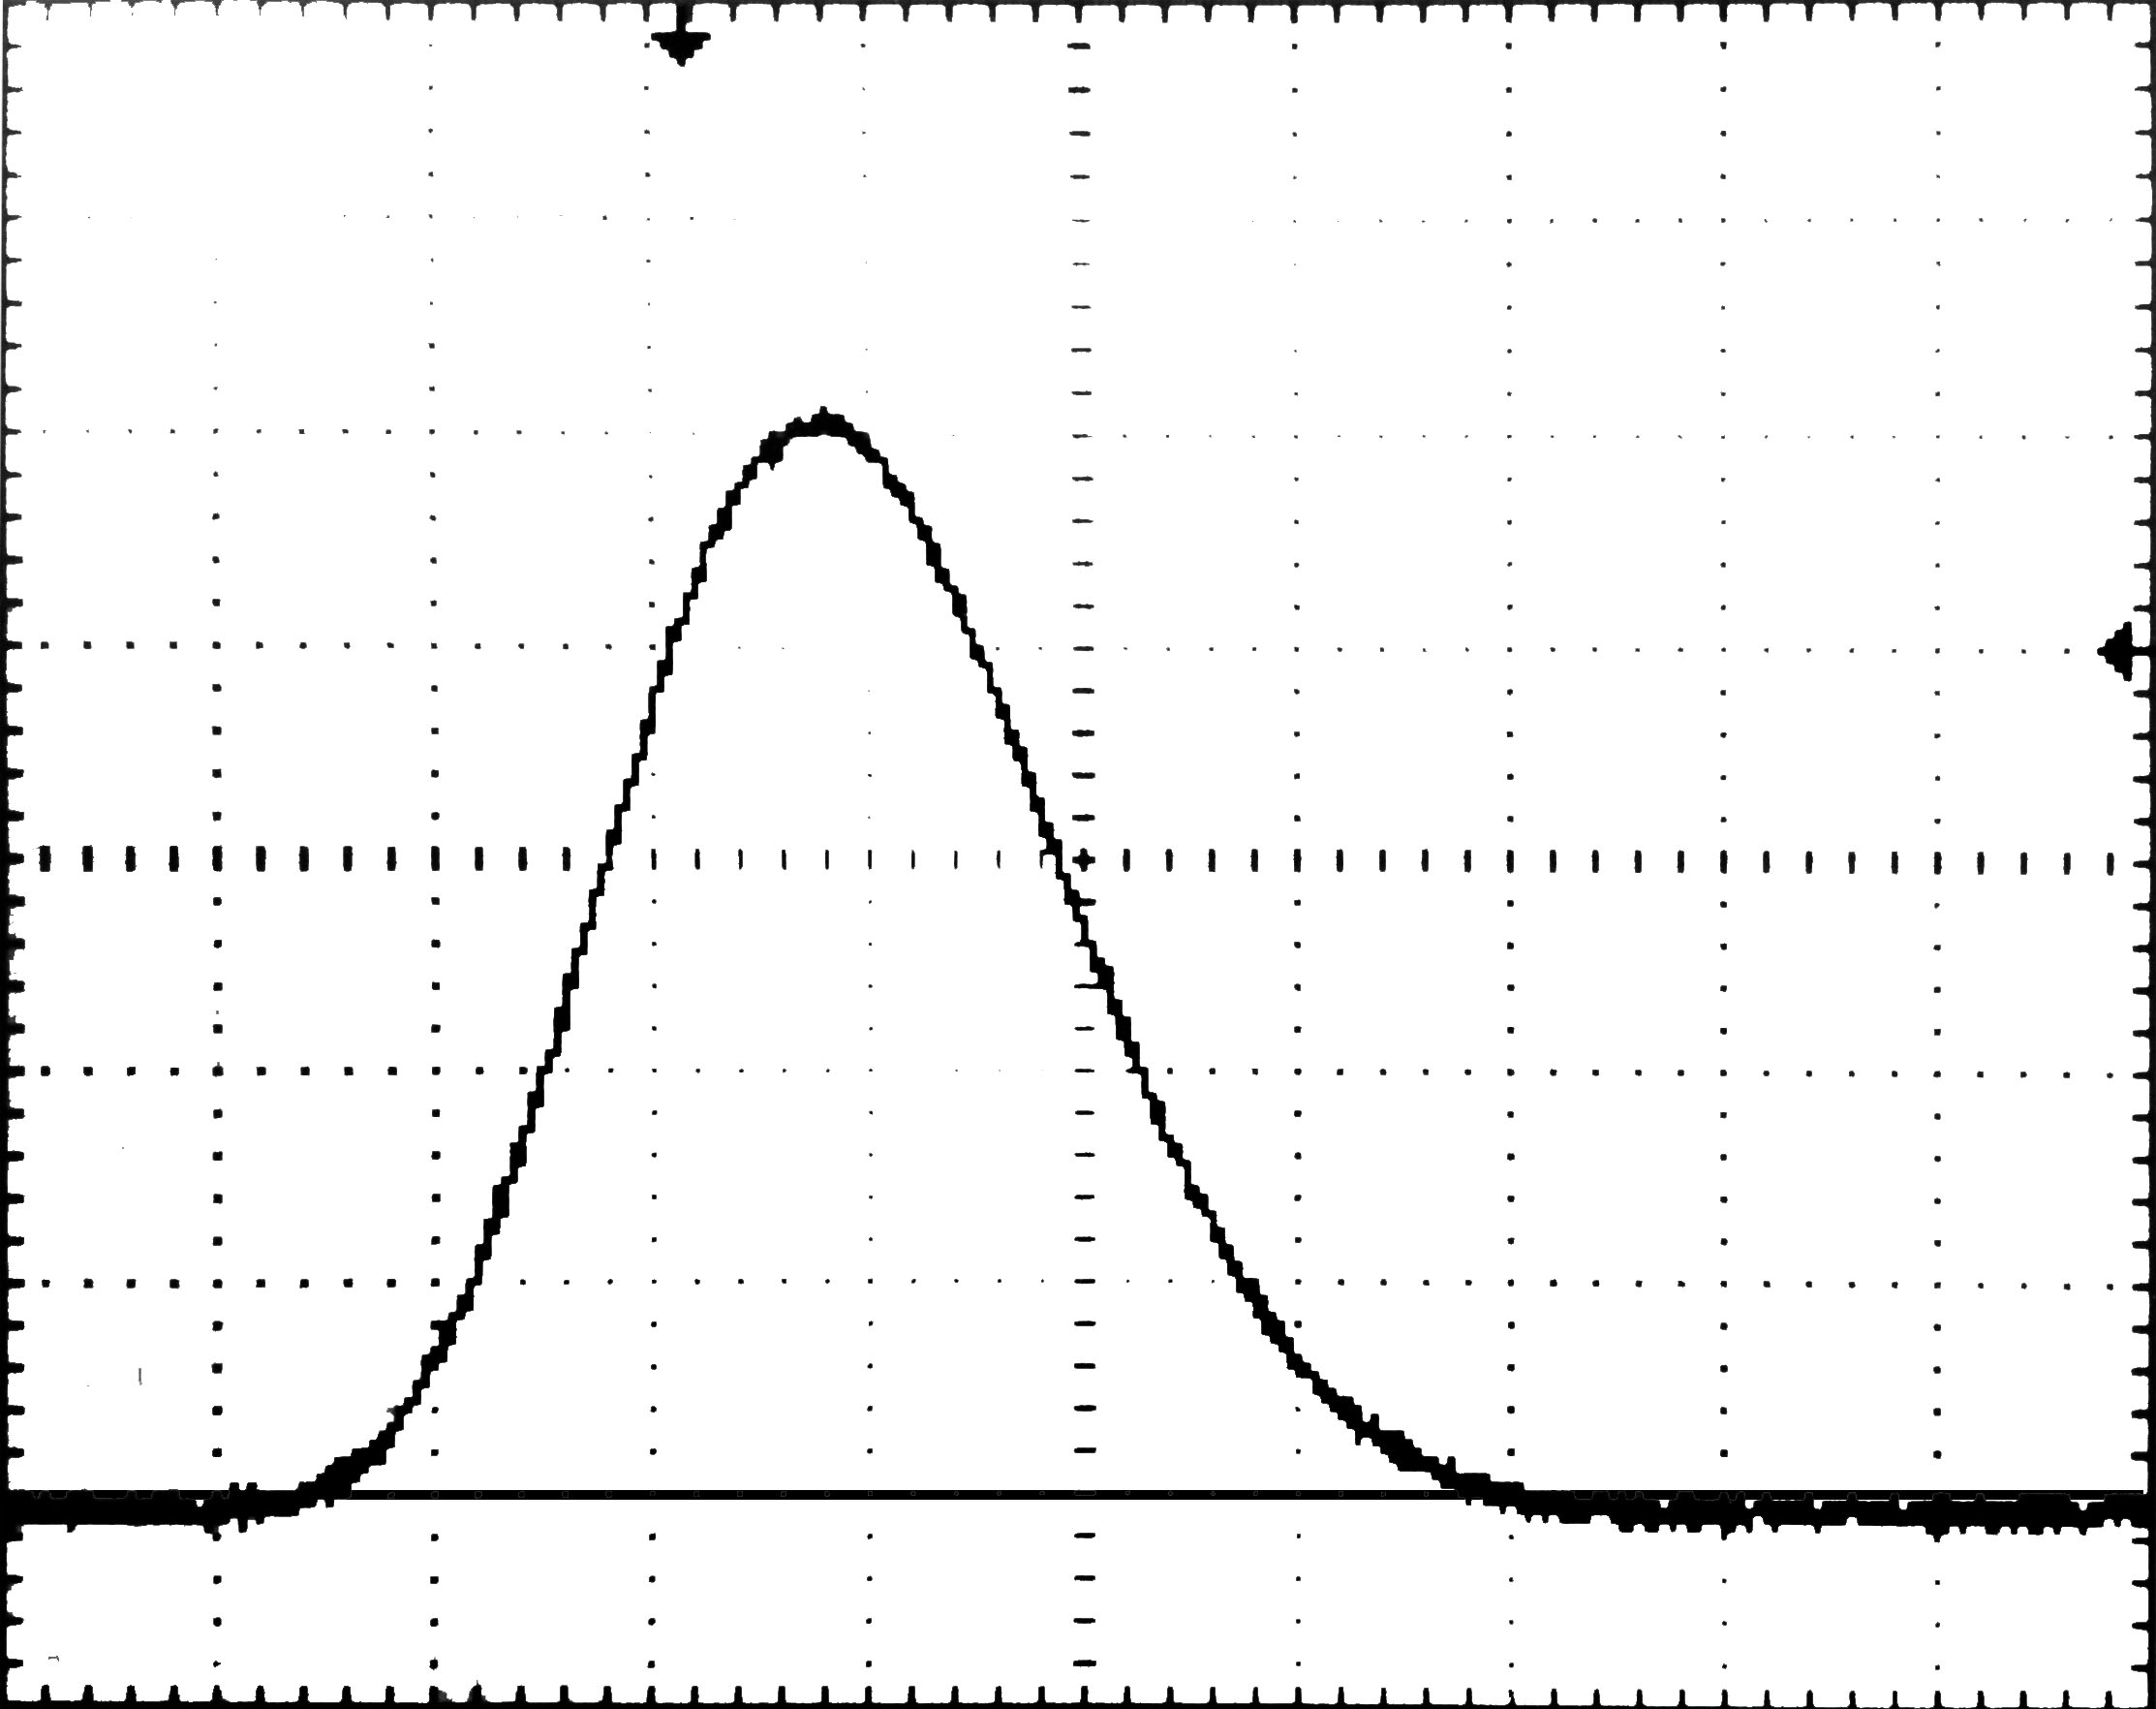
\includegraphics[width=0.7\textwidth]{./figures/signale/haupt_ger_abgeschnitten.jpg}
		\caption{Am Ausgang des Hauptverstärkers. Die eingestellten Skalenfaktoren am Oszilloskop betragen \SI{1}{\volt\per\division} für die Vertikale und \SI{5}{\micro\second\per\division} in der Horizontalen.}
		\label{fig:signal_ger_haupt}
	\end{subfigure}
	\caption{Signalformen am Halbleiterdetektor. Die horizontalen Linien markieren \SI{0}{\volt}.}
\end{figure}
Betrachtet man nun das Signal am Hauptverstärker in Abbildung \ref{fig:signal_ger_haupt} so beobachtet man einen gaußförmigen Impuls mit einer Signalamplitude von $\Delta U = \SI{5.1 +- 0.2}{\volt}$ und einer Signaldauer von $\Delta t = \SI{22 +- 1}{\micro\second}$.
Im Gegensatz zum Hauptverstärker des Szintillationsdetektors kann kein Überschwingen am unipolaren Ausgang des Verstärkers beobachtet werden.
Man beobachtet eine Kürzung des Signals durch den Hauptverstärker um etwa eine Größenordnung.
Der Vergleich der Impulshöhen macht auch hier wenig Sinn, da diese von unabhängigen Ereignissen stammen, dennoch sollte diese proportional zur im Halbleiter deponierten Energie sein.

\subsubsection{Aufnahme der Gammaspektren (QUELLEN) und des Untergrundspektrums}
\begin{table}[h]
	\centering
	\begin{tabular}{lSS}
\toprule
Isotop & {$d / \si{cm}$} & {$\Delta d / \si{cm}$} \\ \midrule
\isotope[60]{Co} & 3.0 & 0.2 \\
\isotope[137]{Cs} & 20.1 & 0.2 \\
\isotope[152]{Eu} & 22.8 & 0.2 \\ \bottomrule
\end{tabular}
	\caption{Abstände $d$ der Proben vom Halbleiterdetektor}
	\label{tab:abstand_halbleiterdetektor}
\end{table}

\subsubsection{Energiekalibrierung}
\label{sec:kalibrierung_halb}
\begin{figure}[ht]
	\centering
	\resizebox{0.85\textwidth}{!}{
		% GNUPLOT: LaTeX picture with Postscript
\begingroup
  \makeatletter
  \providecommand\color[2][]{%
    \GenericError{(gnuplot) \space\space\space\@spaces}{%
      Package color not loaded in conjunction with
      terminal option `colourtext'%
    }{See the gnuplot documentation for explanation.%
    }{Either use 'blacktext' in gnuplot or load the package
      color.sty in LaTeX.}%
    \renewcommand\color[2][]{}%
  }%
  \providecommand\includegraphics[2][]{%
    \GenericError{(gnuplot) \space\space\space\@spaces}{%
      Package graphicx or graphics not loaded%
    }{See the gnuplot documentation for explanation.%
    }{The gnuplot epslatex terminal needs graphicx.sty or graphics.sty.}%
    \renewcommand\includegraphics[2][]{}%
  }%
  \providecommand\rotatebox[2]{#2}%
  \@ifundefined{ifGPcolor}{%
    \newif\ifGPcolor
    \GPcolortrue
  }{}%
  \@ifundefined{ifGPblacktext}{%
    \newif\ifGPblacktext
    \GPblacktexttrue
  }{}%
  % define a \g@addto@macro without @ in the name:
  \let\gplgaddtomacro\g@addto@macro
  % define empty templates for all commands taking text:
  \gdef\gplbacktext{}%
  \gdef\gplfronttext{}%
  \makeatother
  \ifGPblacktext
    % no textcolor at all
    \def\colorrgb#1{}%
    \def\colorgray#1{}%
  \else
    % gray or color?
    \ifGPcolor
      \def\colorrgb#1{\color[rgb]{#1}}%
      \def\colorgray#1{\color[gray]{#1}}%
      \expandafter\def\csname LTw\endcsname{\color{white}}%
      \expandafter\def\csname LTb\endcsname{\color{black}}%
      \expandafter\def\csname LTa\endcsname{\color{black}}%
      \expandafter\def\csname LT0\endcsname{\color[rgb]{1,0,0}}%
      \expandafter\def\csname LT1\endcsname{\color[rgb]{0,1,0}}%
      \expandafter\def\csname LT2\endcsname{\color[rgb]{0,0,1}}%
      \expandafter\def\csname LT3\endcsname{\color[rgb]{1,0,1}}%
      \expandafter\def\csname LT4\endcsname{\color[rgb]{0,1,1}}%
      \expandafter\def\csname LT5\endcsname{\color[rgb]{1,1,0}}%
      \expandafter\def\csname LT6\endcsname{\color[rgb]{0,0,0}}%
      \expandafter\def\csname LT7\endcsname{\color[rgb]{1,0.3,0}}%
      \expandafter\def\csname LT8\endcsname{\color[rgb]{0.5,0.5,0.5}}%
    \else
      % gray
      \def\colorrgb#1{\color{black}}%
      \def\colorgray#1{\color[gray]{#1}}%
      \expandafter\def\csname LTw\endcsname{\color{white}}%
      \expandafter\def\csname LTb\endcsname{\color{black}}%
      \expandafter\def\csname LTa\endcsname{\color{black}}%
      \expandafter\def\csname LT0\endcsname{\color{black}}%
      \expandafter\def\csname LT1\endcsname{\color{black}}%
      \expandafter\def\csname LT2\endcsname{\color{black}}%
      \expandafter\def\csname LT3\endcsname{\color{black}}%
      \expandafter\def\csname LT4\endcsname{\color{black}}%
      \expandafter\def\csname LT5\endcsname{\color{black}}%
      \expandafter\def\csname LT6\endcsname{\color{black}}%
      \expandafter\def\csname LT7\endcsname{\color{black}}%
      \expandafter\def\csname LT8\endcsname{\color{black}}%
    \fi
  \fi
    \setlength{\unitlength}{0.0500bp}%
    \ifx\gptboxheight\undefined%
      \newlength{\gptboxheight}%
      \newlength{\gptboxwidth}%
      \newsavebox{\gptboxtext}%
    \fi%
    \setlength{\fboxrule}{0.5pt}%
    \setlength{\fboxsep}{1pt}%
\begin{picture}(7488.00,5040.00)%
    \gplgaddtomacro\gplbacktext{%
      \csname LTb\endcsname%
      \put(1078,704){\makebox(0,0)[r]{\strut{}$0$}}%
      \csname LTb\endcsname%
      \put(1078,1286){\makebox(0,0)[r]{\strut{}$5000$}}%
      \csname LTb\endcsname%
      \put(1078,1867){\makebox(0,0)[r]{\strut{}$10000$}}%
      \csname LTb\endcsname%
      \put(1078,2449){\makebox(0,0)[r]{\strut{}$15000$}}%
      \csname LTb\endcsname%
      \put(1078,3030){\makebox(0,0)[r]{\strut{}$20000$}}%
      \csname LTb\endcsname%
      \put(1078,3612){\makebox(0,0)[r]{\strut{}$25000$}}%
      \csname LTb\endcsname%
      \put(1078,4193){\makebox(0,0)[r]{\strut{}$30000$}}%
      \csname LTb\endcsname%
      \put(1078,4775){\makebox(0,0)[r]{\strut{}$35000$}}%
      \csname LTb\endcsname%
      \put(1210,484){\makebox(0,0){\strut{}$3255$}}%
      \csname LTb\endcsname%
      \put(2190,484){\makebox(0,0){\strut{}$3260$}}%
      \csname LTb\endcsname%
      \put(3170,484){\makebox(0,0){\strut{}$3265$}}%
      \csname LTb\endcsname%
      \put(4151,484){\makebox(0,0){\strut{}$3270$}}%
      \csname LTb\endcsname%
      \put(5131,484){\makebox(0,0){\strut{}$3275$}}%
      \csname LTb\endcsname%
      \put(6111,484){\makebox(0,0){\strut{}$3280$}}%
      \csname LTb\endcsname%
      \put(7091,484){\makebox(0,0){\strut{}$3285$}}%
    }%
    \gplgaddtomacro\gplfronttext{%
      \csname LTb\endcsname%
      \put(176,2739){\rotatebox{-270}{\makebox(0,0){\strut{}Ereignisse $N$}}}%
      \put(4150,154){\makebox(0,0){\strut{}Kanalnummer $n$}}%
      \put(4150,4665){\makebox(0,0){\strut{}}}%
      \csname LTb\endcsname%
      \put(2530,4602){\makebox(0,0)[r]{\strut{}Messwerte}}%
      \csname LTb\endcsname%
      \put(2530,4382){\makebox(0,0)[r]{\strut{}$\Sigma$}}%
      \csname LTb\endcsname%
      \put(2530,4162){\makebox(0,0)[r]{\strut{}$\mathcal{G}$}}%
      \csname LTb\endcsname%
      \put(2530,3942){\makebox(0,0)[r]{\strut{}$d$}}%
    }%
    \gplbacktext
    \put(0,0){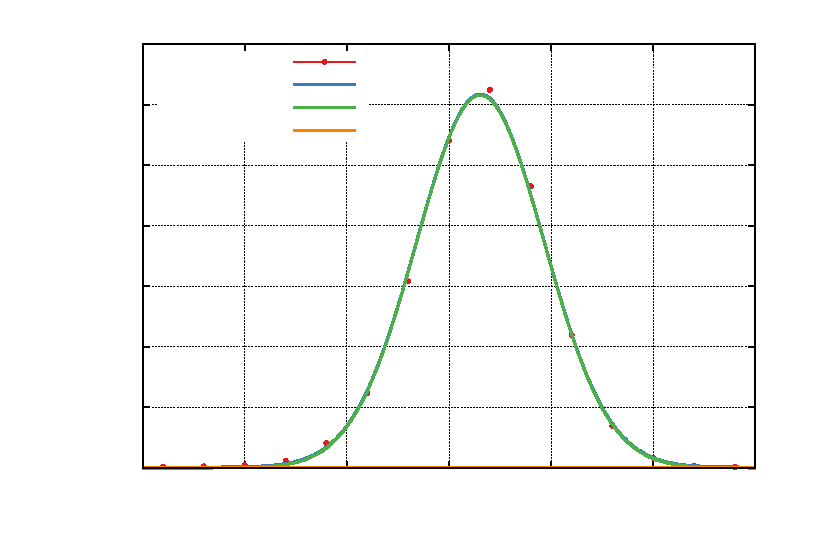
\includegraphics{./plots/halbleiter/energiekalibrierung/caesium_darstellung}}%
    \gplfronttext
  \end{picture}%
\endgroup

	}
	\caption{Anpassung für die Linie im Gammaspektrum von Caesium}
	\label{fig:fit_caesium}
\end{figure}
Wie beim Sztintillationsdetektor wird auch für den Halbeiterdetektor eine Energiekalibrierung durchgeführt, indem an die gefundenen Linien im Gammaspektrum der Proben eine Kurve der Form \eqref{eq:gaussfithypothese} angepasst wird.
Im Gegensatz zum NaI(Tl)-Detektor kann jedoch auch die Europiumlinie von \SI{1085.914}{\kilo\electronvolt} deutlich gesehen und zur Kalibrierung genutzt werden.
Es ergeben sich die in Tabelle \ref{tab:kalibrierungslinien_halb} festgehaltenen Werte für die Anpassungen und zugehörigen Gammaenergien aller drei Quellen.
\begin{table}[ht]
	\centering
	\resizebox{\textwidth}{!}{
	\begin{tabular}{lSSSSSSS}
	\toprule
	Isotop & {Gammaenergie} & \multicolumn{2}{c}{Amplitude} & \multicolumn{2}{c}{Schwerpunkt} & \multicolumn{2}{c}{Standardabweichung}\\
	& {$E_{\gamma}$ / \si{\kilo\electronvolt}} & {$A$} & {$\Delta A$} & {$n$} & {$\Delta n$} & {$\sigma$} & {$\Delta \sigma$}\\
	\midrule
Co & 1173.237 & 10512.8 & 241.6 & 5819.34 & 0.07 & 3.94 & 0.07 \\
Co & 1332.501 & 8750.2  & 230.6 & 6612.25 & 0.07 & 4.25 & 0.08 \\
Cs & 661.660  & 30775.2 & 394.3 & 3271.54 & 0.03 & 3.12 & 0.03 \\
Eu & 121.783  & 23990.4 & 605.3 & 583.33  & 0.05 & 2.18 & 0.05 \\
Eu & 244.699  & 4660.0  & 99.6  & 1195.92 & 0.05 & 2.35 & 0.05 \\
Eu & 344.281  & 11083.5 & 174.0 & 1691.53 & 0.04 & 2.61 & 0.03 \\
Eu & 778.903  & 2008.9  & 30.3  & 3854.90 & 0.05 & 3.24 & 0.04 \\
Eu & 964.131  & 1796.2  & 29.5  & 4777.38 & 0.05 & 3.48 & 0.05 \\
Eu & 1085.914 & 1055.9  & 18.1  & 5384.05 & 0.06 & 3.66 & 0.06 \\
Eu & 1112.116 & 1332.3  & 37.9  & 5514.44 & 0.09 & 3.78 & 0.09 \\
Eu & 1408.011 & 1534.0  & 33.5  & 6987.49 & 0.06 & 4.17 & 0.07 \\
	\bottomrule
\end{tabular}
	}
	\caption{Anpassungsergebnisse zur Energiekalibrierung für den Ge-Halbleiterdetektor}
	\label{tab:kalibrierungslinien_halb}
\end{table}
Da die Daten offensichtlich einen linearen Zusammenhang auf dem gesamten Bereich nahelegen, wird zur Anpassung eine lineare Funktion der Form $mx + b$ gewählt (analog zum NaI(Tl) Detektor).
Das Ergebnis der Anpassung ist in Abbildung \ref{fig:kalibrierung_halb} zu sehen.
\begin{figure}[ht]
	\centering
	\begin{tabular}{lSSSSSSS}
	\toprule
	Isotop & {Gammaenergie} & \multicolumn{2}{c}{Amplitude} & \multicolumn{2}{c}{Schwerpunkt} & \multicolumn{2}{c}{Standardabweichung}\\
	& {$E_{\gamma}$ / \si{\kilo\electronvolt}} & {$A$} & {$\Delta A$} & {$n$} & {$\Delta n$} & {$\sigma$} & {$\Delta \sigma$}\\
	\midrule
Co & 1173.237 & 10512.8 & 241.6 & 5819.34 & 0.07 & 3.94 & 0.07 \\
Co & 1332.501 & 8750.2  & 230.6 & 6612.25 & 0.07 & 4.25 & 0.08 \\
Cs & 661.660  & 30775.2 & 394.3 & 3271.54 & 0.03 & 3.12 & 0.03 \\
Eu & 121.783  & 23990.4 & 605.3 & 583.33  & 0.05 & 2.18 & 0.05 \\
Eu & 244.699  & 4660.0  & 99.6  & 1195.92 & 0.05 & 2.35 & 0.05 \\
Eu & 344.281  & 11083.5 & 174.0 & 1691.53 & 0.04 & 2.61 & 0.03 \\
Eu & 778.903  & 2008.9  & 30.3  & 3854.90 & 0.05 & 3.24 & 0.04 \\
Eu & 964.131  & 1796.2  & 29.5  & 4777.38 & 0.05 & 3.48 & 0.05 \\
Eu & 1085.914 & 1055.9  & 18.1  & 5384.05 & 0.06 & 3.66 & 0.06 \\
Eu & 1112.116 & 1332.3  & 37.9  & 5514.44 & 0.09 & 3.78 & 0.09 \\
Eu & 1408.011 & 1534.0  & 33.5  & 6987.49 & 0.06 & 4.17 & 0.07 \\
	\bottomrule
\end{tabular}
	\caption{Energiekalibrierung des Ge-Halbleiterdetektors. Die Fehler sind zu klein, um gesehen werden zu können.}
	\label{fig:kalibrierung_halb}
\end{figure}  
Anpassungsergebnisse \texttt{gnuplot}:
\begin{align}
	m &= \SI{0.200839 +- 0.000013}{\kilo\electronvolt} \\
	b &= \SI{4.561 +- 0.059}{\kilo\electronvolt}
\end{align}


\subsubsection{Bestimmung der Halbwertsbreite}
Zur Bestimmung der Halbwertsbreiten für den Halbleiterdetektor kann erneut die Anpassung der Gaußfunktionen an die jeweiligen Linien verwendet werden, welche bereits bei der Energiekalibrierung in Abschnitt \ref{sec:kalibrierung_halb} durchgeführt wurden.
Analog zum Szintillationsdetektor wird dabei die volle Halbwertsbreite (FWHM) aus der Standardabweichung $\sigma$ der Anpassung berechnet.
Mit den Anpassungsergebnissen aus Tabelle \ref{tab:kalibrierungslinien_halb} kann dementsprechend die Halbwertsbreite in Einheiten der Kanalnummer berechnet werden.
Diese kann mithilfe der Energiekalibrierung in Abschnitt \ref{sec:kalibrierung_halb} in Einheiten der Energie umgerechnet werden, indem die Halbwertsbreite in Einheiten der Kanalnummer mit der Steigung der Kalibrierungsgeraden multipliziert wird.
Die berechneten Breiten wurden in Tabelle \ref{tab:fwhm_halb} zusammengetragen.
\begin{table}[ht]
	\centering
	\begin{tabular}{lSSSSS}
\toprule
Isotop & {Gammaenergie} & {FWHM} & {$\Delta \text{FWHM}$} & {FWHM} & {$\Delta \text{FWHM}$}\\
       & {$E_\gamma$ / \si{keV}}             & \multicolumn{2}{c}{Kanäle} & \multicolumn{2}{c}{\si{keV}} \\
\midrule
Co & 1173.237 & 9.28  & 0.16 & 1.864 & 0.031 \\
Co & 1332.501 & 10.00 & 0.19 & 2.008 & 0.037 \\
Cs & 661.660  & 7.34  & 0.07 & 1.475 & 0.013 \\
Eu & 121.783  & 5.12  & 0.10 & 1.029 & 0.020 \\
Eu & 244.699  & 5.54  & 0.11 & 1.113 & 0.021 \\
Eu & 344.281  & 6.14  & 0.07 & 1.232 & 0.014 \\
Eu & 778.903  & 7.63  & 0.10 & 1.533 & 0.019 \\
Eu & 964.131  & 8.19  & 0.11 & 1.645 & 0.021 \\
Eu & 1085.914 & 8.62  & 0.13 & 1.731 & 0.026 \\
Eu & 1112.116 & 8.90  & 0.20 & 1.787 & 0.039 \\
Eu & 1408.011 & 9.82  & 0.15 & 1.972 & 0.031 \\
\bottomrule
\end{tabular}
	\caption{Volle Halbwertsbreiten der zur Kalibration verwendeten Linien in den Spektren von \isotope[60]{Co}, \isotope[137]{Cs} und \isotope[152]{Eu}.}
	\label{tab:fwhm_halb}
\end{table}

\begin{figure}[h]
	\centering
	% GNUPLOT: LaTeX picture with Postscript
\begingroup
  \makeatletter
  \providecommand\color[2][]{%
    \GenericError{(gnuplot) \space\space\space\@spaces}{%
      Package color not loaded in conjunction with
      terminal option `colourtext'%
    }{See the gnuplot documentation for explanation.%
    }{Either use 'blacktext' in gnuplot or load the package
      color.sty in LaTeX.}%
    \renewcommand\color[2][]{}%
  }%
  \providecommand\includegraphics[2][]{%
    \GenericError{(gnuplot) \space\space\space\@spaces}{%
      Package graphicx or graphics not loaded%
    }{See the gnuplot documentation for explanation.%
    }{The gnuplot epslatex terminal needs graphicx.sty or graphics.sty.}%
    \renewcommand\includegraphics[2][]{}%
  }%
  \providecommand\rotatebox[2]{#2}%
  \@ifundefined{ifGPcolor}{%
    \newif\ifGPcolor
    \GPcolortrue
  }{}%
  \@ifundefined{ifGPblacktext}{%
    \newif\ifGPblacktext
    \GPblacktexttrue
  }{}%
  % define a \g@addto@macro without @ in the name:
  \let\gplgaddtomacro\g@addto@macro
  % define empty templates for all commands taking text:
  \gdef\gplbacktext{}%
  \gdef\gplfronttext{}%
  \makeatother
  \ifGPblacktext
    % no textcolor at all
    \def\colorrgb#1{}%
    \def\colorgray#1{}%
  \else
    % gray or color?
    \ifGPcolor
      \def\colorrgb#1{\color[rgb]{#1}}%
      \def\colorgray#1{\color[gray]{#1}}%
      \expandafter\def\csname LTw\endcsname{\color{white}}%
      \expandafter\def\csname LTb\endcsname{\color{black}}%
      \expandafter\def\csname LTa\endcsname{\color{black}}%
      \expandafter\def\csname LT0\endcsname{\color[rgb]{1,0,0}}%
      \expandafter\def\csname LT1\endcsname{\color[rgb]{0,1,0}}%
      \expandafter\def\csname LT2\endcsname{\color[rgb]{0,0,1}}%
      \expandafter\def\csname LT3\endcsname{\color[rgb]{1,0,1}}%
      \expandafter\def\csname LT4\endcsname{\color[rgb]{0,1,1}}%
      \expandafter\def\csname LT5\endcsname{\color[rgb]{1,1,0}}%
      \expandafter\def\csname LT6\endcsname{\color[rgb]{0,0,0}}%
      \expandafter\def\csname LT7\endcsname{\color[rgb]{1,0.3,0}}%
      \expandafter\def\csname LT8\endcsname{\color[rgb]{0.5,0.5,0.5}}%
    \else
      % gray
      \def\colorrgb#1{\color{black}}%
      \def\colorgray#1{\color[gray]{#1}}%
      \expandafter\def\csname LTw\endcsname{\color{white}}%
      \expandafter\def\csname LTb\endcsname{\color{black}}%
      \expandafter\def\csname LTa\endcsname{\color{black}}%
      \expandafter\def\csname LT0\endcsname{\color{black}}%
      \expandafter\def\csname LT1\endcsname{\color{black}}%
      \expandafter\def\csname LT2\endcsname{\color{black}}%
      \expandafter\def\csname LT3\endcsname{\color{black}}%
      \expandafter\def\csname LT4\endcsname{\color{black}}%
      \expandafter\def\csname LT5\endcsname{\color{black}}%
      \expandafter\def\csname LT6\endcsname{\color{black}}%
      \expandafter\def\csname LT7\endcsname{\color{black}}%
      \expandafter\def\csname LT8\endcsname{\color{black}}%
    \fi
  \fi
    \setlength{\unitlength}{0.0500bp}%
    \ifx\gptboxheight\undefined%
      \newlength{\gptboxheight}%
      \newlength{\gptboxwidth}%
      \newsavebox{\gptboxtext}%
    \fi%
    \setlength{\fboxrule}{0.5pt}%
    \setlength{\fboxsep}{1pt}%
\begin{picture}(7200.00,5040.00)%
    \gplgaddtomacro\gplbacktext{%
      \csname LTb\endcsname%
      \put(814,704){\makebox(0,0)[r]{\strut{}$0$}}%
      \csname LTb\endcsname%
      \put(814,1156){\makebox(0,0)[r]{\strut{}$0{,}5$}}%
      \csname LTb\endcsname%
      \put(814,1609){\makebox(0,0)[r]{\strut{}$1$}}%
      \csname LTb\endcsname%
      \put(814,2061){\makebox(0,0)[r]{\strut{}$1{,}5$}}%
      \csname LTb\endcsname%
      \put(814,2513){\makebox(0,0)[r]{\strut{}$2$}}%
      \csname LTb\endcsname%
      \put(814,2966){\makebox(0,0)[r]{\strut{}$2{,}5$}}%
      \csname LTb\endcsname%
      \put(814,3418){\makebox(0,0)[r]{\strut{}$3$}}%
      \csname LTb\endcsname%
      \put(814,3870){\makebox(0,0)[r]{\strut{}$3{,}5$}}%
      \csname LTb\endcsname%
      \put(814,4323){\makebox(0,0)[r]{\strut{}$4$}}%
      \csname LTb\endcsname%
      \put(814,4775){\makebox(0,0)[r]{\strut{}$4{,}5$}}%
      \csname LTb\endcsname%
      \put(946,484){\makebox(0,0){\strut{}$0$}}%
      \csname LTb\endcsname%
      \put(1678,484){\makebox(0,0){\strut{}$200$}}%
      \csname LTb\endcsname%
      \put(2410,484){\makebox(0,0){\strut{}$400$}}%
      \csname LTb\endcsname%
      \put(3142,484){\makebox(0,0){\strut{}$600$}}%
      \csname LTb\endcsname%
      \put(3875,484){\makebox(0,0){\strut{}$800$}}%
      \csname LTb\endcsname%
      \put(4607,484){\makebox(0,0){\strut{}$1000$}}%
      \csname LTb\endcsname%
      \put(5339,484){\makebox(0,0){\strut{}$1200$}}%
      \csname LTb\endcsname%
      \put(6071,484){\makebox(0,0){\strut{}$1400$}}%
      \csname LTb\endcsname%
      \put(6803,484){\makebox(0,0){\strut{}$1600$}}%
    }%
    \gplgaddtomacro\gplfronttext{%
      \csname LTb\endcsname%
      \put(176,2739){\rotatebox{-270}{\makebox(0,0){\strut{}Halbwertsbreite $\Delta E^2$}}}%
      \put(3874,154){\makebox(0,0){\strut{}Gammaenergie $E_\gamma$}}%
      \csname LTb\endcsname%
      \put(2266,4602){\makebox(0,0)[r]{\strut{}Messwerte}}%
      \csname LTb\endcsname%
      \put(2266,4382){\makebox(0,0)[r]{\strut{}Anpassung}}%
    }%
    \gplbacktext
    \put(0,0){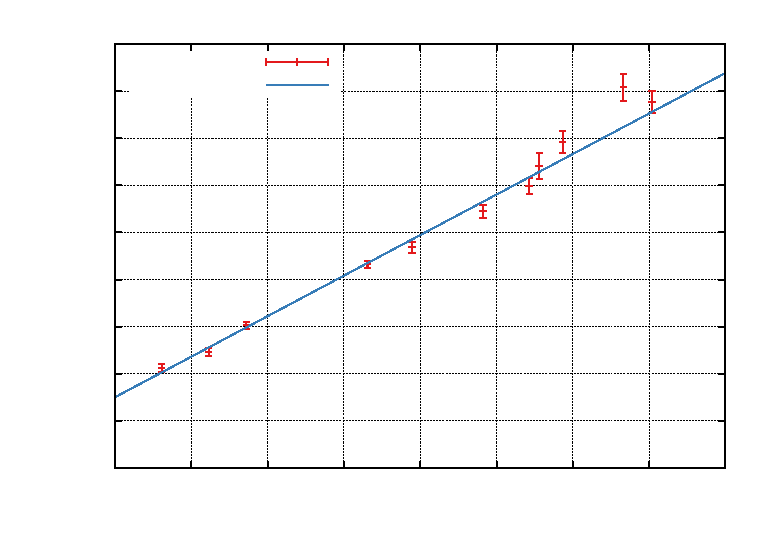
\includegraphics{./plots/halbleiter/linearisierung_halbwertsbreiten}}%
    \gplfronttext
  \end{picture}%
\endgroup

	\caption{Linearisierung}
	\label{fig:lin_fwhm}
\end{figure}


\subsubsection{Intrinsische Halbwertsbreite}

\subsubsection{Peak-to-Total-Verhältnis}

\subsubsection{Absolute Peakeffizienz}

\subsubsection{Relative Effizienz als Funktion der Gammaenergie}

\subsection{Nachweis der Radioakivität in einer Probe}

\section{Fazit}

\begin{figure}[h]
	\centering
	% GNUPLOT: LaTeX picture with Postscript
\begingroup
  \makeatletter
  \providecommand\color[2][]{%
    \GenericError{(gnuplot) \space\space\space\@spaces}{%
      Package color not loaded in conjunction with
      terminal option `colourtext'%
    }{See the gnuplot documentation for explanation.%
    }{Either use 'blacktext' in gnuplot or load the package
      color.sty in LaTeX.}%
    \renewcommand\color[2][]{}%
  }%
  \providecommand\includegraphics[2][]{%
    \GenericError{(gnuplot) \space\space\space\@spaces}{%
      Package graphicx or graphics not loaded%
    }{See the gnuplot documentation for explanation.%
    }{The gnuplot epslatex terminal needs graphicx.sty or graphics.sty.}%
    \renewcommand\includegraphics[2][]{}%
  }%
  \providecommand\rotatebox[2]{#2}%
  \@ifundefined{ifGPcolor}{%
    \newif\ifGPcolor
    \GPcolortrue
  }{}%
  \@ifundefined{ifGPblacktext}{%
    \newif\ifGPblacktext
    \GPblacktexttrue
  }{}%
  % define a \g@addto@macro without @ in the name:
  \let\gplgaddtomacro\g@addto@macro
  % define empty templates for all commands taking text:
  \gdef\gplbacktext{}%
  \gdef\gplfronttext{}%
  \makeatother
  \ifGPblacktext
    % no textcolor at all
    \def\colorrgb#1{}%
    \def\colorgray#1{}%
  \else
    % gray or color?
    \ifGPcolor
      \def\colorrgb#1{\color[rgb]{#1}}%
      \def\colorgray#1{\color[gray]{#1}}%
      \expandafter\def\csname LTw\endcsname{\color{white}}%
      \expandafter\def\csname LTb\endcsname{\color{black}}%
      \expandafter\def\csname LTa\endcsname{\color{black}}%
      \expandafter\def\csname LT0\endcsname{\color[rgb]{1,0,0}}%
      \expandafter\def\csname LT1\endcsname{\color[rgb]{0,1,0}}%
      \expandafter\def\csname LT2\endcsname{\color[rgb]{0,0,1}}%
      \expandafter\def\csname LT3\endcsname{\color[rgb]{1,0,1}}%
      \expandafter\def\csname LT4\endcsname{\color[rgb]{0,1,1}}%
      \expandafter\def\csname LT5\endcsname{\color[rgb]{1,1,0}}%
      \expandafter\def\csname LT6\endcsname{\color[rgb]{0,0,0}}%
      \expandafter\def\csname LT7\endcsname{\color[rgb]{1,0.3,0}}%
      \expandafter\def\csname LT8\endcsname{\color[rgb]{0.5,0.5,0.5}}%
    \else
      % gray
      \def\colorrgb#1{\color{black}}%
      \def\colorgray#1{\color[gray]{#1}}%
      \expandafter\def\csname LTw\endcsname{\color{white}}%
      \expandafter\def\csname LTb\endcsname{\color{black}}%
      \expandafter\def\csname LTa\endcsname{\color{black}}%
      \expandafter\def\csname LT0\endcsname{\color{black}}%
      \expandafter\def\csname LT1\endcsname{\color{black}}%
      \expandafter\def\csname LT2\endcsname{\color{black}}%
      \expandafter\def\csname LT3\endcsname{\color{black}}%
      \expandafter\def\csname LT4\endcsname{\color{black}}%
      \expandafter\def\csname LT5\endcsname{\color{black}}%
      \expandafter\def\csname LT6\endcsname{\color{black}}%
      \expandafter\def\csname LT7\endcsname{\color{black}}%
      \expandafter\def\csname LT8\endcsname{\color{black}}%
    \fi
  \fi
    \setlength{\unitlength}{0.0500bp}%
    \ifx\gptboxheight\undefined%
      \newlength{\gptboxheight}%
      \newlength{\gptboxwidth}%
      \newsavebox{\gptboxtext}%
    \fi%
    \setlength{\fboxrule}{0.5pt}%
    \setlength{\fboxsep}{1pt}%
\begin{picture}(7200.00,5040.00)%
    \gplgaddtomacro\gplbacktext{%
      \csname LTb\endcsname%
      \put(946,704){\makebox(0,0)[r]{\strut{}$0$}}%
      \csname LTb\endcsname%
      \put(946,1286){\makebox(0,0)[r]{\strut{}$200$}}%
      \csname LTb\endcsname%
      \put(946,1867){\makebox(0,0)[r]{\strut{}$400$}}%
      \csname LTb\endcsname%
      \put(946,2449){\makebox(0,0)[r]{\strut{}$600$}}%
      \csname LTb\endcsname%
      \put(946,3030){\makebox(0,0)[r]{\strut{}$800$}}%
      \csname LTb\endcsname%
      \put(946,3612){\makebox(0,0)[r]{\strut{}$1000$}}%
      \csname LTb\endcsname%
      \put(946,4193){\makebox(0,0)[r]{\strut{}$1200$}}%
      \csname LTb\endcsname%
      \put(946,4775){\makebox(0,0)[r]{\strut{}$1400$}}%
      \csname LTb\endcsname%
      \put(1078,484){\makebox(0,0){\strut{}$0$}}%
      \csname LTb\endcsname%
      \put(2223,484){\makebox(0,0){\strut{}$1000$}}%
      \csname LTb\endcsname%
      \put(3368,484){\makebox(0,0){\strut{}$2000$}}%
      \csname LTb\endcsname%
      \put(4513,484){\makebox(0,0){\strut{}$3000$}}%
      \csname LTb\endcsname%
      \put(5658,484){\makebox(0,0){\strut{}$4000$}}%
      \csname LTb\endcsname%
      \put(6803,484){\makebox(0,0){\strut{}$5000$}}%
    }%
    \gplgaddtomacro\gplfronttext{%
      \csname LTb\endcsname%
      \put(176,2739){\rotatebox{-270}{\makebox(0,0){\strut{}Ereignisse $N$}}}%
      \put(3940,154){\makebox(0,0){\strut{}Kanal $n$}}%
      \csname LTb\endcsname%
      \put(5816,4602){\makebox(0,0)[r]{\strut{}Messwerte}}%
    }%
    \gplbacktext
    \put(0,0){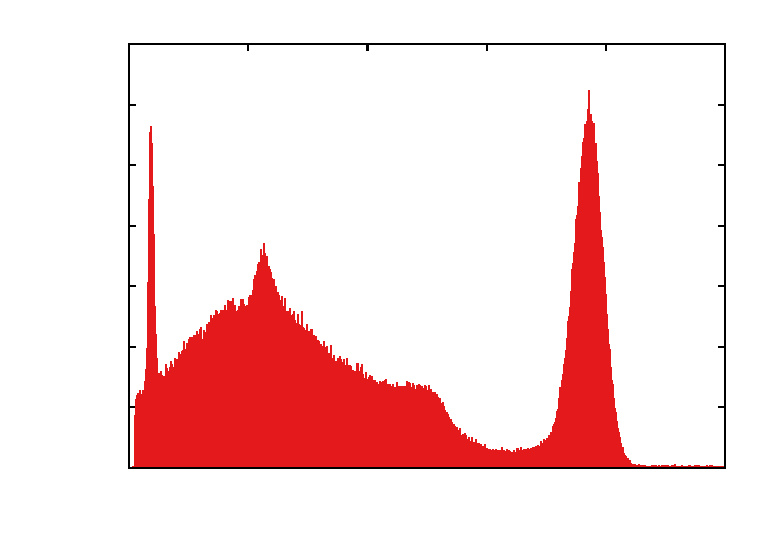
\includegraphics{./plots/szintillator/caesium}}%
    \gplfronttext
  \end{picture}%
\endgroup

	\caption{Cääääääsium szinti}
	\label{fig:szin_caesium_spektrum}
\end{figure}

\begin{figure}[h]
	\centering
	% GNUPLOT: LaTeX picture with Postscript
\begingroup
  \makeatletter
  \providecommand\color[2][]{%
    \GenericError{(gnuplot) \space\space\space\@spaces}{%
      Package color not loaded in conjunction with
      terminal option `colourtext'%
    }{See the gnuplot documentation for explanation.%
    }{Either use 'blacktext' in gnuplot or load the package
      color.sty in LaTeX.}%
    \renewcommand\color[2][]{}%
  }%
  \providecommand\includegraphics[2][]{%
    \GenericError{(gnuplot) \space\space\space\@spaces}{%
      Package graphicx or graphics not loaded%
    }{See the gnuplot documentation for explanation.%
    }{The gnuplot epslatex terminal needs graphicx.sty or graphics.sty.}%
    \renewcommand\includegraphics[2][]{}%
  }%
  \providecommand\rotatebox[2]{#2}%
  \@ifundefined{ifGPcolor}{%
    \newif\ifGPcolor
    \GPcolortrue
  }{}%
  \@ifundefined{ifGPblacktext}{%
    \newif\ifGPblacktext
    \GPblacktexttrue
  }{}%
  % define a \g@addto@macro without @ in the name:
  \let\gplgaddtomacro\g@addto@macro
  % define empty templates for all commands taking text:
  \gdef\gplbacktext{}%
  \gdef\gplfronttext{}%
  \makeatother
  \ifGPblacktext
    % no textcolor at all
    \def\colorrgb#1{}%
    \def\colorgray#1{}%
  \else
    % gray or color?
    \ifGPcolor
      \def\colorrgb#1{\color[rgb]{#1}}%
      \def\colorgray#1{\color[gray]{#1}}%
      \expandafter\def\csname LTw\endcsname{\color{white}}%
      \expandafter\def\csname LTb\endcsname{\color{black}}%
      \expandafter\def\csname LTa\endcsname{\color{black}}%
      \expandafter\def\csname LT0\endcsname{\color[rgb]{1,0,0}}%
      \expandafter\def\csname LT1\endcsname{\color[rgb]{0,1,0}}%
      \expandafter\def\csname LT2\endcsname{\color[rgb]{0,0,1}}%
      \expandafter\def\csname LT3\endcsname{\color[rgb]{1,0,1}}%
      \expandafter\def\csname LT4\endcsname{\color[rgb]{0,1,1}}%
      \expandafter\def\csname LT5\endcsname{\color[rgb]{1,1,0}}%
      \expandafter\def\csname LT6\endcsname{\color[rgb]{0,0,0}}%
      \expandafter\def\csname LT7\endcsname{\color[rgb]{1,0.3,0}}%
      \expandafter\def\csname LT8\endcsname{\color[rgb]{0.5,0.5,0.5}}%
    \else
      % gray
      \def\colorrgb#1{\color{black}}%
      \def\colorgray#1{\color[gray]{#1}}%
      \expandafter\def\csname LTw\endcsname{\color{white}}%
      \expandafter\def\csname LTb\endcsname{\color{black}}%
      \expandafter\def\csname LTa\endcsname{\color{black}}%
      \expandafter\def\csname LT0\endcsname{\color{black}}%
      \expandafter\def\csname LT1\endcsname{\color{black}}%
      \expandafter\def\csname LT2\endcsname{\color{black}}%
      \expandafter\def\csname LT3\endcsname{\color{black}}%
      \expandafter\def\csname LT4\endcsname{\color{black}}%
      \expandafter\def\csname LT5\endcsname{\color{black}}%
      \expandafter\def\csname LT6\endcsname{\color{black}}%
      \expandafter\def\csname LT7\endcsname{\color{black}}%
      \expandafter\def\csname LT8\endcsname{\color{black}}%
    \fi
  \fi
    \setlength{\unitlength}{0.0500bp}%
    \ifx\gptboxheight\undefined%
      \newlength{\gptboxheight}%
      \newlength{\gptboxwidth}%
      \newsavebox{\gptboxtext}%
    \fi%
    \setlength{\fboxrule}{0.5pt}%
    \setlength{\fboxsep}{1pt}%
\begin{picture}(7200.00,5040.00)%
    \gplgaddtomacro\gplbacktext{%
      \csname LTb\endcsname%
      \put(1078,704){\makebox(0,0)[r]{\strut{}$0$}}%
      \csname LTb\endcsname%
      \put(1078,1383){\makebox(0,0)[r]{\strut{}$2000$}}%
      \csname LTb\endcsname%
      \put(1078,2061){\makebox(0,0)[r]{\strut{}$4000$}}%
      \csname LTb\endcsname%
      \put(1078,2740){\makebox(0,0)[r]{\strut{}$6000$}}%
      \csname LTb\endcsname%
      \put(1078,3418){\makebox(0,0)[r]{\strut{}$8000$}}%
      \csname LTb\endcsname%
      \put(1078,4097){\makebox(0,0)[r]{\strut{}$10000$}}%
      \csname LTb\endcsname%
      \put(1078,4775){\makebox(0,0)[r]{\strut{}$12000$}}%
      \csname LTb\endcsname%
      \put(1210,484){\makebox(0,0){\strut{}$0$}}%
      \csname LTb\endcsname%
      \put(1831,484){\makebox(0,0){\strut{}$1000$}}%
      \csname LTb\endcsname%
      \put(2453,484){\makebox(0,0){\strut{}$2000$}}%
      \csname LTb\endcsname%
      \put(3074,484){\makebox(0,0){\strut{}$3000$}}%
      \csname LTb\endcsname%
      \put(3696,484){\makebox(0,0){\strut{}$4000$}}%
      \csname LTb\endcsname%
      \put(4317,484){\makebox(0,0){\strut{}$5000$}}%
      \csname LTb\endcsname%
      \put(4939,484){\makebox(0,0){\strut{}$6000$}}%
      \csname LTb\endcsname%
      \put(5560,484){\makebox(0,0){\strut{}$7000$}}%
      \csname LTb\endcsname%
      \put(6182,484){\makebox(0,0){\strut{}$8000$}}%
      \csname LTb\endcsname%
      \put(6803,484){\makebox(0,0){\strut{}$9000$}}%
    }%
    \gplgaddtomacro\gplfronttext{%
      \csname LTb\endcsname%
      \put(176,2739){\rotatebox{-270}{\makebox(0,0){\strut{}Ereignisse $$}}}%
      \put(4006,154){\makebox(0,0){\strut{}Kanal $n$}}%
      \csname LTb\endcsname%
      \put(2530,4602){\makebox(0,0)[r]{\strut{}Messwerte}}%
    }%
    \gplbacktext
    \put(0,0){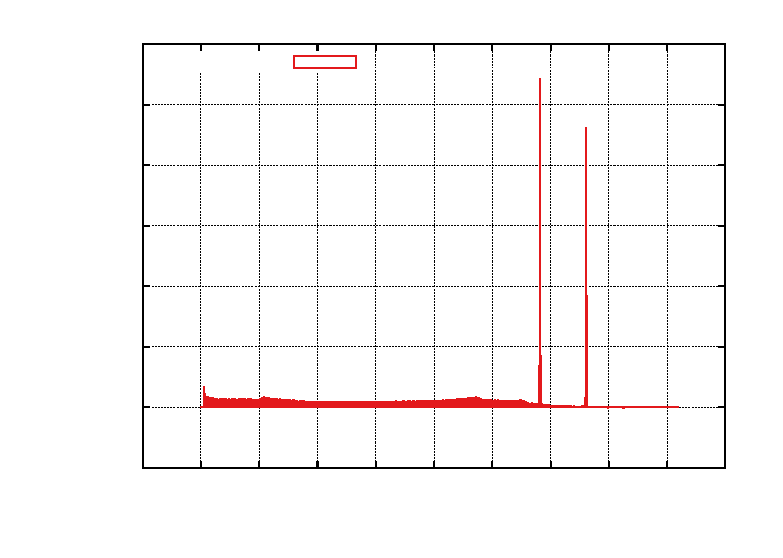
\includegraphics{./plots/halbleiter/cobalt}}%
    \gplfronttext
  \end{picture}%
\endgroup

	\caption{Cooooobalt szinti}
	\label{fig:szin_cobalt_spektrum}
\end{figure}

\begin{figure}[h]
	\centering
	% GNUPLOT: LaTeX picture with Postscript
\begingroup
  \makeatletter
  \providecommand\color[2][]{%
    \GenericError{(gnuplot) \space\space\space\@spaces}{%
      Package color not loaded in conjunction with
      terminal option `colourtext'%
    }{See the gnuplot documentation for explanation.%
    }{Either use 'blacktext' in gnuplot or load the package
      color.sty in LaTeX.}%
    \renewcommand\color[2][]{}%
  }%
  \providecommand\includegraphics[2][]{%
    \GenericError{(gnuplot) \space\space\space\@spaces}{%
      Package graphicx or graphics not loaded%
    }{See the gnuplot documentation for explanation.%
    }{The gnuplot epslatex terminal needs graphicx.sty or graphics.sty.}%
    \renewcommand\includegraphics[2][]{}%
  }%
  \providecommand\rotatebox[2]{#2}%
  \@ifundefined{ifGPcolor}{%
    \newif\ifGPcolor
    \GPcolortrue
  }{}%
  \@ifundefined{ifGPblacktext}{%
    \newif\ifGPblacktext
    \GPblacktexttrue
  }{}%
  % define a \g@addto@macro without @ in the name:
  \let\gplgaddtomacro\g@addto@macro
  % define empty templates for all commands taking text:
  \gdef\gplbacktext{}%
  \gdef\gplfronttext{}%
  \makeatother
  \ifGPblacktext
    % no textcolor at all
    \def\colorrgb#1{}%
    \def\colorgray#1{}%
  \else
    % gray or color?
    \ifGPcolor
      \def\colorrgb#1{\color[rgb]{#1}}%
      \def\colorgray#1{\color[gray]{#1}}%
      \expandafter\def\csname LTw\endcsname{\color{white}}%
      \expandafter\def\csname LTb\endcsname{\color{black}}%
      \expandafter\def\csname LTa\endcsname{\color{black}}%
      \expandafter\def\csname LT0\endcsname{\color[rgb]{1,0,0}}%
      \expandafter\def\csname LT1\endcsname{\color[rgb]{0,1,0}}%
      \expandafter\def\csname LT2\endcsname{\color[rgb]{0,0,1}}%
      \expandafter\def\csname LT3\endcsname{\color[rgb]{1,0,1}}%
      \expandafter\def\csname LT4\endcsname{\color[rgb]{0,1,1}}%
      \expandafter\def\csname LT5\endcsname{\color[rgb]{1,1,0}}%
      \expandafter\def\csname LT6\endcsname{\color[rgb]{0,0,0}}%
      \expandafter\def\csname LT7\endcsname{\color[rgb]{1,0.3,0}}%
      \expandafter\def\csname LT8\endcsname{\color[rgb]{0.5,0.5,0.5}}%
    \else
      % gray
      \def\colorrgb#1{\color{black}}%
      \def\colorgray#1{\color[gray]{#1}}%
      \expandafter\def\csname LTw\endcsname{\color{white}}%
      \expandafter\def\csname LTb\endcsname{\color{black}}%
      \expandafter\def\csname LTa\endcsname{\color{black}}%
      \expandafter\def\csname LT0\endcsname{\color{black}}%
      \expandafter\def\csname LT1\endcsname{\color{black}}%
      \expandafter\def\csname LT2\endcsname{\color{black}}%
      \expandafter\def\csname LT3\endcsname{\color{black}}%
      \expandafter\def\csname LT4\endcsname{\color{black}}%
      \expandafter\def\csname LT5\endcsname{\color{black}}%
      \expandafter\def\csname LT6\endcsname{\color{black}}%
      \expandafter\def\csname LT7\endcsname{\color{black}}%
      \expandafter\def\csname LT8\endcsname{\color{black}}%
    \fi
  \fi
    \setlength{\unitlength}{0.0500bp}%
    \ifx\gptboxheight\undefined%
      \newlength{\gptboxheight}%
      \newlength{\gptboxwidth}%
      \newsavebox{\gptboxtext}%
    \fi%
    \setlength{\fboxrule}{0.5pt}%
    \setlength{\fboxsep}{1pt}%
\begin{picture}(7200.00,5040.00)%
    \gplgaddtomacro\gplbacktext{%
      \csname LTb\endcsname%
      \put(946,704){\makebox(0,0)[r]{\strut{}$0$}}%
      \put(946,1156){\makebox(0,0)[r]{\strut{}$500$}}%
      \put(946,1609){\makebox(0,0)[r]{\strut{}$1000$}}%
      \put(946,2061){\makebox(0,0)[r]{\strut{}$1500$}}%
      \put(946,2513){\makebox(0,0)[r]{\strut{}$2000$}}%
      \put(946,2966){\makebox(0,0)[r]{\strut{}$2500$}}%
      \put(946,3418){\makebox(0,0)[r]{\strut{}$3000$}}%
      \put(946,3870){\makebox(0,0)[r]{\strut{}$3500$}}%
      \put(946,4323){\makebox(0,0)[r]{\strut{}$4000$}}%
      \put(946,4775){\makebox(0,0)[r]{\strut{}$4500$}}%
      \put(1078,484){\makebox(0,0){\strut{}$0$}}%
      \put(1896,484){\makebox(0,0){\strut{}$1000$}}%
      \put(2714,484){\makebox(0,0){\strut{}$2000$}}%
      \put(3532,484){\makebox(0,0){\strut{}$3000$}}%
      \put(4349,484){\makebox(0,0){\strut{}$4000$}}%
      \put(5167,484){\makebox(0,0){\strut{}$5000$}}%
      \put(5985,484){\makebox(0,0){\strut{}$6000$}}%
      \put(6803,484){\makebox(0,0){\strut{}$7000$}}%
      \put(1413,3508){\rotatebox{-270}{\makebox(0,0)[l]{\strut{}Röntgenlinie}}}%
      \put(1675,2716){\rotatebox{-270}{\makebox(0,0)[l]{\strut{}\SI{121.783}{keV}}}}%
      \put(2256,1240){\rotatebox{-270}{\makebox(0,0)[l]{\strut{}\SI{244.699}{keV}}}}%
      \put(2706,1315){\rotatebox{-270}{\makebox(0,0)[l]{\strut{}\SI{344.281}{keV}}}}%
      \put(4769,930){\rotatebox{-270}{\makebox(0,0)[l]{\strut{}\SI{778.903}{keV}}}}%
      \put(5599,921){\rotatebox{-270}{\makebox(0,0)[l]{\strut{}\SI{964.131}{keV}}}}%
      \put(6006,995){\rotatebox{-270}{\makebox(0,0)[l]{\strut{}\SI{1112.116}{keV}}}}%
      \put(6492,948){\rotatebox{-270}{\makebox(0,0)[l]{\strut{}\SI{1408.011}{keV}}}}%
    }%
    \gplgaddtomacro\gplfronttext{%
      \csname LTb\endcsname%
      \put(176,2739){\rotatebox{-270}{\makebox(0,0){\strut{}Ereignisse $N$}}}%
      \put(3940,154){\makebox(0,0){\strut{}Kanal $n$}}%
    }%
    \gplbacktext
    \put(0,0){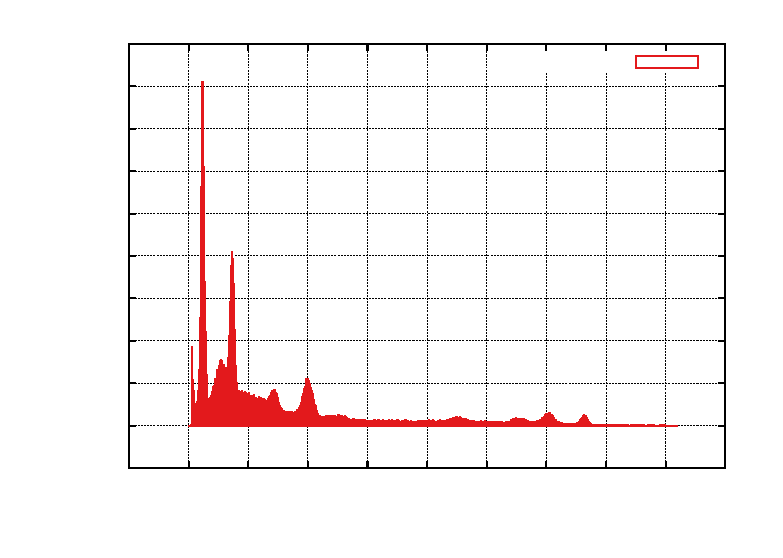
\includegraphics{./plots/szintillator/europium}}%
    \gplfronttext
  \end{picture}%
\endgroup

	\caption{Euroooopium szinti}
	\label{fig:szin_europium_spektrum}
\end{figure}

\begin{figure}[h]
	\centering
	% GNUPLOT: LaTeX picture with Postscript
\begingroup
  \makeatletter
  \providecommand\color[2][]{%
    \GenericError{(gnuplot) \space\space\space\@spaces}{%
      Package color not loaded in conjunction with
      terminal option `colourtext'%
    }{See the gnuplot documentation for explanation.%
    }{Either use 'blacktext' in gnuplot or load the package
      color.sty in LaTeX.}%
    \renewcommand\color[2][]{}%
  }%
  \providecommand\includegraphics[2][]{%
    \GenericError{(gnuplot) \space\space\space\@spaces}{%
      Package graphicx or graphics not loaded%
    }{See the gnuplot documentation for explanation.%
    }{The gnuplot epslatex terminal needs graphicx.sty or graphics.sty.}%
    \renewcommand\includegraphics[2][]{}%
  }%
  \providecommand\rotatebox[2]{#2}%
  \@ifundefined{ifGPcolor}{%
    \newif\ifGPcolor
    \GPcolortrue
  }{}%
  \@ifundefined{ifGPblacktext}{%
    \newif\ifGPblacktext
    \GPblacktexttrue
  }{}%
  % define a \g@addto@macro without @ in the name:
  \let\gplgaddtomacro\g@addto@macro
  % define empty templates for all commands taking text:
  \gdef\gplbacktext{}%
  \gdef\gplfronttext{}%
  \makeatother
  \ifGPblacktext
    % no textcolor at all
    \def\colorrgb#1{}%
    \def\colorgray#1{}%
  \else
    % gray or color?
    \ifGPcolor
      \def\colorrgb#1{\color[rgb]{#1}}%
      \def\colorgray#1{\color[gray]{#1}}%
      \expandafter\def\csname LTw\endcsname{\color{white}}%
      \expandafter\def\csname LTb\endcsname{\color{black}}%
      \expandafter\def\csname LTa\endcsname{\color{black}}%
      \expandafter\def\csname LT0\endcsname{\color[rgb]{1,0,0}}%
      \expandafter\def\csname LT1\endcsname{\color[rgb]{0,1,0}}%
      \expandafter\def\csname LT2\endcsname{\color[rgb]{0,0,1}}%
      \expandafter\def\csname LT3\endcsname{\color[rgb]{1,0,1}}%
      \expandafter\def\csname LT4\endcsname{\color[rgb]{0,1,1}}%
      \expandafter\def\csname LT5\endcsname{\color[rgb]{1,1,0}}%
      \expandafter\def\csname LT6\endcsname{\color[rgb]{0,0,0}}%
      \expandafter\def\csname LT7\endcsname{\color[rgb]{1,0.3,0}}%
      \expandafter\def\csname LT8\endcsname{\color[rgb]{0.5,0.5,0.5}}%
    \else
      % gray
      \def\colorrgb#1{\color{black}}%
      \def\colorgray#1{\color[gray]{#1}}%
      \expandafter\def\csname LTw\endcsname{\color{white}}%
      \expandafter\def\csname LTb\endcsname{\color{black}}%
      \expandafter\def\csname LTa\endcsname{\color{black}}%
      \expandafter\def\csname LT0\endcsname{\color{black}}%
      \expandafter\def\csname LT1\endcsname{\color{black}}%
      \expandafter\def\csname LT2\endcsname{\color{black}}%
      \expandafter\def\csname LT3\endcsname{\color{black}}%
      \expandafter\def\csname LT4\endcsname{\color{black}}%
      \expandafter\def\csname LT5\endcsname{\color{black}}%
      \expandafter\def\csname LT6\endcsname{\color{black}}%
      \expandafter\def\csname LT7\endcsname{\color{black}}%
      \expandafter\def\csname LT8\endcsname{\color{black}}%
    \fi
  \fi
    \setlength{\unitlength}{0.0500bp}%
    \ifx\gptboxheight\undefined%
      \newlength{\gptboxheight}%
      \newlength{\gptboxwidth}%
      \newsavebox{\gptboxtext}%
    \fi%
    \setlength{\fboxrule}{0.5pt}%
    \setlength{\fboxsep}{1pt}%
\begin{picture}(7200.00,5040.00)%
    \gplgaddtomacro\gplbacktext{%
      \csname LTb\endcsname%
      \put(946,704){\makebox(0,0)[r]{\strut{}$0$}}%
      \csname LTb\endcsname%
      \put(946,1286){\makebox(0,0)[r]{\strut{}$200$}}%
      \csname LTb\endcsname%
      \put(946,1867){\makebox(0,0)[r]{\strut{}$400$}}%
      \csname LTb\endcsname%
      \put(946,2449){\makebox(0,0)[r]{\strut{}$600$}}%
      \csname LTb\endcsname%
      \put(946,3030){\makebox(0,0)[r]{\strut{}$800$}}%
      \csname LTb\endcsname%
      \put(946,3612){\makebox(0,0)[r]{\strut{}$1000$}}%
      \csname LTb\endcsname%
      \put(946,4193){\makebox(0,0)[r]{\strut{}$1200$}}%
      \csname LTb\endcsname%
      \put(946,4775){\makebox(0,0)[r]{\strut{}$1400$}}%
      \csname LTb\endcsname%
      \put(1078,484){\makebox(0,0){\strut{}$0$}}%
      \csname LTb\endcsname%
      \put(2223,484){\makebox(0,0){\strut{}$1000$}}%
      \csname LTb\endcsname%
      \put(3368,484){\makebox(0,0){\strut{}$2000$}}%
      \csname LTb\endcsname%
      \put(4513,484){\makebox(0,0){\strut{}$3000$}}%
      \csname LTb\endcsname%
      \put(5658,484){\makebox(0,0){\strut{}$4000$}}%
      \csname LTb\endcsname%
      \put(6803,484){\makebox(0,0){\strut{}$5000$}}%
    }%
    \gplgaddtomacro\gplfronttext{%
      \csname LTb\endcsname%
      \put(176,2739){\rotatebox{-270}{\makebox(0,0){\strut{}Ereignisse $N$}}}%
      \put(3940,154){\makebox(0,0){\strut{}Kanal $n$}}%
      \csname LTb\endcsname%
      \put(5816,4602){\makebox(0,0)[r]{\strut{}Messwerte}}%
    }%
    \gplbacktext
    \put(0,0){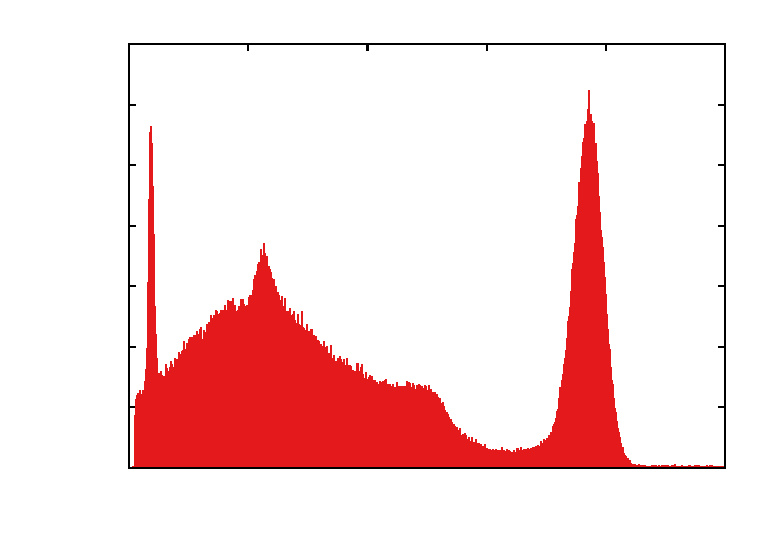
\includegraphics{./plots/szintillator/caesium}}%
    \gplfronttext
  \end{picture}%
\endgroup

	\caption{Cääääääsium halbleiter}
	\label{fig:halb_caesium_spektrum}
\end{figure}

\begin{figure}[h]
	\centering
	% GNUPLOT: LaTeX picture with Postscript
\begingroup
  \makeatletter
  \providecommand\color[2][]{%
    \GenericError{(gnuplot) \space\space\space\@spaces}{%
      Package color not loaded in conjunction with
      terminal option `colourtext'%
    }{See the gnuplot documentation for explanation.%
    }{Either use 'blacktext' in gnuplot or load the package
      color.sty in LaTeX.}%
    \renewcommand\color[2][]{}%
  }%
  \providecommand\includegraphics[2][]{%
    \GenericError{(gnuplot) \space\space\space\@spaces}{%
      Package graphicx or graphics not loaded%
    }{See the gnuplot documentation for explanation.%
    }{The gnuplot epslatex terminal needs graphicx.sty or graphics.sty.}%
    \renewcommand\includegraphics[2][]{}%
  }%
  \providecommand\rotatebox[2]{#2}%
  \@ifundefined{ifGPcolor}{%
    \newif\ifGPcolor
    \GPcolortrue
  }{}%
  \@ifundefined{ifGPblacktext}{%
    \newif\ifGPblacktext
    \GPblacktexttrue
  }{}%
  % define a \g@addto@macro without @ in the name:
  \let\gplgaddtomacro\g@addto@macro
  % define empty templates for all commands taking text:
  \gdef\gplbacktext{}%
  \gdef\gplfronttext{}%
  \makeatother
  \ifGPblacktext
    % no textcolor at all
    \def\colorrgb#1{}%
    \def\colorgray#1{}%
  \else
    % gray or color?
    \ifGPcolor
      \def\colorrgb#1{\color[rgb]{#1}}%
      \def\colorgray#1{\color[gray]{#1}}%
      \expandafter\def\csname LTw\endcsname{\color{white}}%
      \expandafter\def\csname LTb\endcsname{\color{black}}%
      \expandafter\def\csname LTa\endcsname{\color{black}}%
      \expandafter\def\csname LT0\endcsname{\color[rgb]{1,0,0}}%
      \expandafter\def\csname LT1\endcsname{\color[rgb]{0,1,0}}%
      \expandafter\def\csname LT2\endcsname{\color[rgb]{0,0,1}}%
      \expandafter\def\csname LT3\endcsname{\color[rgb]{1,0,1}}%
      \expandafter\def\csname LT4\endcsname{\color[rgb]{0,1,1}}%
      \expandafter\def\csname LT5\endcsname{\color[rgb]{1,1,0}}%
      \expandafter\def\csname LT6\endcsname{\color[rgb]{0,0,0}}%
      \expandafter\def\csname LT7\endcsname{\color[rgb]{1,0.3,0}}%
      \expandafter\def\csname LT8\endcsname{\color[rgb]{0.5,0.5,0.5}}%
    \else
      % gray
      \def\colorrgb#1{\color{black}}%
      \def\colorgray#1{\color[gray]{#1}}%
      \expandafter\def\csname LTw\endcsname{\color{white}}%
      \expandafter\def\csname LTb\endcsname{\color{black}}%
      \expandafter\def\csname LTa\endcsname{\color{black}}%
      \expandafter\def\csname LT0\endcsname{\color{black}}%
      \expandafter\def\csname LT1\endcsname{\color{black}}%
      \expandafter\def\csname LT2\endcsname{\color{black}}%
      \expandafter\def\csname LT3\endcsname{\color{black}}%
      \expandafter\def\csname LT4\endcsname{\color{black}}%
      \expandafter\def\csname LT5\endcsname{\color{black}}%
      \expandafter\def\csname LT6\endcsname{\color{black}}%
      \expandafter\def\csname LT7\endcsname{\color{black}}%
      \expandafter\def\csname LT8\endcsname{\color{black}}%
    \fi
  \fi
    \setlength{\unitlength}{0.0500bp}%
    \ifx\gptboxheight\undefined%
      \newlength{\gptboxheight}%
      \newlength{\gptboxwidth}%
      \newsavebox{\gptboxtext}%
    \fi%
    \setlength{\fboxrule}{0.5pt}%
    \setlength{\fboxsep}{1pt}%
\begin{picture}(7200.00,5040.00)%
    \gplgaddtomacro\gplbacktext{%
      \csname LTb\endcsname%
      \put(1078,704){\makebox(0,0)[r]{\strut{}$0$}}%
      \csname LTb\endcsname%
      \put(1078,1383){\makebox(0,0)[r]{\strut{}$2000$}}%
      \csname LTb\endcsname%
      \put(1078,2061){\makebox(0,0)[r]{\strut{}$4000$}}%
      \csname LTb\endcsname%
      \put(1078,2740){\makebox(0,0)[r]{\strut{}$6000$}}%
      \csname LTb\endcsname%
      \put(1078,3418){\makebox(0,0)[r]{\strut{}$8000$}}%
      \csname LTb\endcsname%
      \put(1078,4097){\makebox(0,0)[r]{\strut{}$10000$}}%
      \csname LTb\endcsname%
      \put(1078,4775){\makebox(0,0)[r]{\strut{}$12000$}}%
      \csname LTb\endcsname%
      \put(1210,484){\makebox(0,0){\strut{}$0$}}%
      \csname LTb\endcsname%
      \put(1831,484){\makebox(0,0){\strut{}$1000$}}%
      \csname LTb\endcsname%
      \put(2453,484){\makebox(0,0){\strut{}$2000$}}%
      \csname LTb\endcsname%
      \put(3074,484){\makebox(0,0){\strut{}$3000$}}%
      \csname LTb\endcsname%
      \put(3696,484){\makebox(0,0){\strut{}$4000$}}%
      \csname LTb\endcsname%
      \put(4317,484){\makebox(0,0){\strut{}$5000$}}%
      \csname LTb\endcsname%
      \put(4939,484){\makebox(0,0){\strut{}$6000$}}%
      \csname LTb\endcsname%
      \put(5560,484){\makebox(0,0){\strut{}$7000$}}%
      \csname LTb\endcsname%
      \put(6182,484){\makebox(0,0){\strut{}$8000$}}%
      \csname LTb\endcsname%
      \put(6803,484){\makebox(0,0){\strut{}$9000$}}%
    }%
    \gplgaddtomacro\gplfronttext{%
      \csname LTb\endcsname%
      \put(176,2739){\rotatebox{-270}{\makebox(0,0){\strut{}Ereignisse $$}}}%
      \put(4006,154){\makebox(0,0){\strut{}Kanal $n$}}%
      \csname LTb\endcsname%
      \put(2530,4602){\makebox(0,0)[r]{\strut{}Messwerte}}%
    }%
    \gplbacktext
    \put(0,0){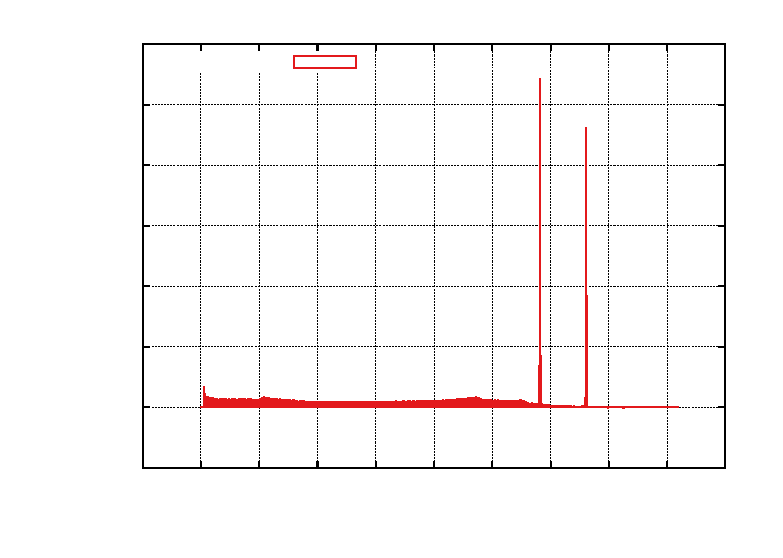
\includegraphics{./plots/halbleiter/cobalt}}%
    \gplfronttext
  \end{picture}%
\endgroup

	\caption{Cooooobalt halbleiter}
	\label{fig:halb_cobalt_spektrum}
\end{figure}

\begin{figure}[h]
	\centering
	% GNUPLOT: LaTeX picture with Postscript
\begingroup
  \makeatletter
  \providecommand\color[2][]{%
    \GenericError{(gnuplot) \space\space\space\@spaces}{%
      Package color not loaded in conjunction with
      terminal option `colourtext'%
    }{See the gnuplot documentation for explanation.%
    }{Either use 'blacktext' in gnuplot or load the package
      color.sty in LaTeX.}%
    \renewcommand\color[2][]{}%
  }%
  \providecommand\includegraphics[2][]{%
    \GenericError{(gnuplot) \space\space\space\@spaces}{%
      Package graphicx or graphics not loaded%
    }{See the gnuplot documentation for explanation.%
    }{The gnuplot epslatex terminal needs graphicx.sty or graphics.sty.}%
    \renewcommand\includegraphics[2][]{}%
  }%
  \providecommand\rotatebox[2]{#2}%
  \@ifundefined{ifGPcolor}{%
    \newif\ifGPcolor
    \GPcolortrue
  }{}%
  \@ifundefined{ifGPblacktext}{%
    \newif\ifGPblacktext
    \GPblacktexttrue
  }{}%
  % define a \g@addto@macro without @ in the name:
  \let\gplgaddtomacro\g@addto@macro
  % define empty templates for all commands taking text:
  \gdef\gplbacktext{}%
  \gdef\gplfronttext{}%
  \makeatother
  \ifGPblacktext
    % no textcolor at all
    \def\colorrgb#1{}%
    \def\colorgray#1{}%
  \else
    % gray or color?
    \ifGPcolor
      \def\colorrgb#1{\color[rgb]{#1}}%
      \def\colorgray#1{\color[gray]{#1}}%
      \expandafter\def\csname LTw\endcsname{\color{white}}%
      \expandafter\def\csname LTb\endcsname{\color{black}}%
      \expandafter\def\csname LTa\endcsname{\color{black}}%
      \expandafter\def\csname LT0\endcsname{\color[rgb]{1,0,0}}%
      \expandafter\def\csname LT1\endcsname{\color[rgb]{0,1,0}}%
      \expandafter\def\csname LT2\endcsname{\color[rgb]{0,0,1}}%
      \expandafter\def\csname LT3\endcsname{\color[rgb]{1,0,1}}%
      \expandafter\def\csname LT4\endcsname{\color[rgb]{0,1,1}}%
      \expandafter\def\csname LT5\endcsname{\color[rgb]{1,1,0}}%
      \expandafter\def\csname LT6\endcsname{\color[rgb]{0,0,0}}%
      \expandafter\def\csname LT7\endcsname{\color[rgb]{1,0.3,0}}%
      \expandafter\def\csname LT8\endcsname{\color[rgb]{0.5,0.5,0.5}}%
    \else
      % gray
      \def\colorrgb#1{\color{black}}%
      \def\colorgray#1{\color[gray]{#1}}%
      \expandafter\def\csname LTw\endcsname{\color{white}}%
      \expandafter\def\csname LTb\endcsname{\color{black}}%
      \expandafter\def\csname LTa\endcsname{\color{black}}%
      \expandafter\def\csname LT0\endcsname{\color{black}}%
      \expandafter\def\csname LT1\endcsname{\color{black}}%
      \expandafter\def\csname LT2\endcsname{\color{black}}%
      \expandafter\def\csname LT3\endcsname{\color{black}}%
      \expandafter\def\csname LT4\endcsname{\color{black}}%
      \expandafter\def\csname LT5\endcsname{\color{black}}%
      \expandafter\def\csname LT6\endcsname{\color{black}}%
      \expandafter\def\csname LT7\endcsname{\color{black}}%
      \expandafter\def\csname LT8\endcsname{\color{black}}%
    \fi
  \fi
    \setlength{\unitlength}{0.0500bp}%
    \ifx\gptboxheight\undefined%
      \newlength{\gptboxheight}%
      \newlength{\gptboxwidth}%
      \newsavebox{\gptboxtext}%
    \fi%
    \setlength{\fboxrule}{0.5pt}%
    \setlength{\fboxsep}{1pt}%
\begin{picture}(7200.00,5040.00)%
    \gplgaddtomacro\gplbacktext{%
      \csname LTb\endcsname%
      \put(946,704){\makebox(0,0)[r]{\strut{}$0$}}%
      \put(946,1156){\makebox(0,0)[r]{\strut{}$500$}}%
      \put(946,1609){\makebox(0,0)[r]{\strut{}$1000$}}%
      \put(946,2061){\makebox(0,0)[r]{\strut{}$1500$}}%
      \put(946,2513){\makebox(0,0)[r]{\strut{}$2000$}}%
      \put(946,2966){\makebox(0,0)[r]{\strut{}$2500$}}%
      \put(946,3418){\makebox(0,0)[r]{\strut{}$3000$}}%
      \put(946,3870){\makebox(0,0)[r]{\strut{}$3500$}}%
      \put(946,4323){\makebox(0,0)[r]{\strut{}$4000$}}%
      \put(946,4775){\makebox(0,0)[r]{\strut{}$4500$}}%
      \put(1078,484){\makebox(0,0){\strut{}$0$}}%
      \put(1896,484){\makebox(0,0){\strut{}$1000$}}%
      \put(2714,484){\makebox(0,0){\strut{}$2000$}}%
      \put(3532,484){\makebox(0,0){\strut{}$3000$}}%
      \put(4349,484){\makebox(0,0){\strut{}$4000$}}%
      \put(5167,484){\makebox(0,0){\strut{}$5000$}}%
      \put(5985,484){\makebox(0,0){\strut{}$6000$}}%
      \put(6803,484){\makebox(0,0){\strut{}$7000$}}%
      \put(1413,3508){\rotatebox{-270}{\makebox(0,0)[l]{\strut{}Röntgenlinie}}}%
      \put(1675,2716){\rotatebox{-270}{\makebox(0,0)[l]{\strut{}\SI{121.783}{keV}}}}%
      \put(2256,1240){\rotatebox{-270}{\makebox(0,0)[l]{\strut{}\SI{244.699}{keV}}}}%
      \put(2706,1315){\rotatebox{-270}{\makebox(0,0)[l]{\strut{}\SI{344.281}{keV}}}}%
      \put(4769,930){\rotatebox{-270}{\makebox(0,0)[l]{\strut{}\SI{778.903}{keV}}}}%
      \put(5599,921){\rotatebox{-270}{\makebox(0,0)[l]{\strut{}\SI{964.131}{keV}}}}%
      \put(6006,995){\rotatebox{-270}{\makebox(0,0)[l]{\strut{}\SI{1112.116}{keV}}}}%
      \put(6492,948){\rotatebox{-270}{\makebox(0,0)[l]{\strut{}\SI{1408.011}{keV}}}}%
    }%
    \gplgaddtomacro\gplfronttext{%
      \csname LTb\endcsname%
      \put(176,2739){\rotatebox{-270}{\makebox(0,0){\strut{}Ereignisse $N$}}}%
      \put(3940,154){\makebox(0,0){\strut{}Kanal $n$}}%
    }%
    \gplbacktext
    \put(0,0){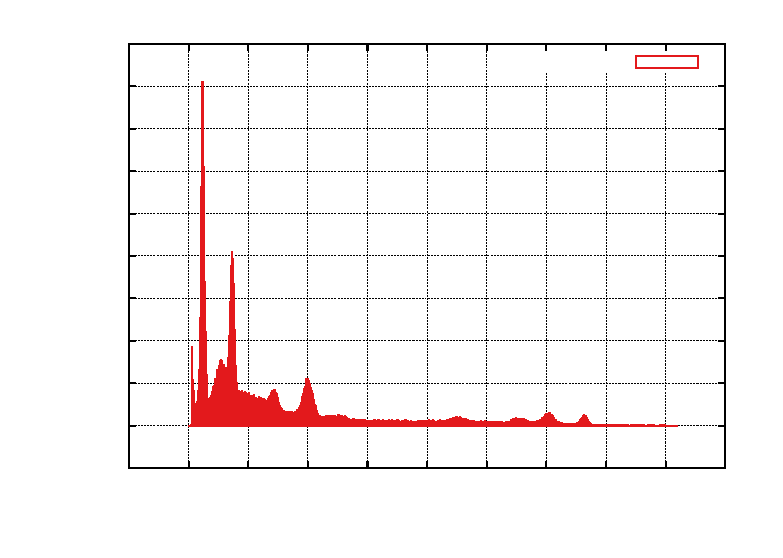
\includegraphics{./plots/szintillator/europium}}%
    \gplfronttext
  \end{picture}%
\endgroup

	\caption{Euroooopium halbleiter}
	\label{fig:halb_europium_spektrum}
\end{figure}

\begin{figure}
	% GNUPLOT: LaTeX picture with Postscript
\begingroup
  \makeatletter
  \providecommand\color[2][]{%
    \GenericError{(gnuplot) \space\space\space\@spaces}{%
      Package color not loaded in conjunction with
      terminal option `colourtext'%
    }{See the gnuplot documentation for explanation.%
    }{Either use 'blacktext' in gnuplot or load the package
      color.sty in LaTeX.}%
    \renewcommand\color[2][]{}%
  }%
  \providecommand\includegraphics[2][]{%
    \GenericError{(gnuplot) \space\space\space\@spaces}{%
      Package graphicx or graphics not loaded%
    }{See the gnuplot documentation for explanation.%
    }{The gnuplot epslatex terminal needs graphicx.sty or graphics.sty.}%
    \renewcommand\includegraphics[2][]{}%
  }%
  \providecommand\rotatebox[2]{#2}%
  \@ifundefined{ifGPcolor}{%
    \newif\ifGPcolor
    \GPcolortrue
  }{}%
  \@ifundefined{ifGPblacktext}{%
    \newif\ifGPblacktext
    \GPblacktexttrue
  }{}%
  % define a \g@addto@macro without @ in the name:
  \let\gplgaddtomacro\g@addto@macro
  % define empty templates for all commands taking text:
  \gdef\gplbacktext{}%
  \gdef\gplfronttext{}%
  \makeatother
  \ifGPblacktext
    % no textcolor at all
    \def\colorrgb#1{}%
    \def\colorgray#1{}%
  \else
    % gray or color?
    \ifGPcolor
      \def\colorrgb#1{\color[rgb]{#1}}%
      \def\colorgray#1{\color[gray]{#1}}%
      \expandafter\def\csname LTw\endcsname{\color{white}}%
      \expandafter\def\csname LTb\endcsname{\color{black}}%
      \expandafter\def\csname LTa\endcsname{\color{black}}%
      \expandafter\def\csname LT0\endcsname{\color[rgb]{1,0,0}}%
      \expandafter\def\csname LT1\endcsname{\color[rgb]{0,1,0}}%
      \expandafter\def\csname LT2\endcsname{\color[rgb]{0,0,1}}%
      \expandafter\def\csname LT3\endcsname{\color[rgb]{1,0,1}}%
      \expandafter\def\csname LT4\endcsname{\color[rgb]{0,1,1}}%
      \expandafter\def\csname LT5\endcsname{\color[rgb]{1,1,0}}%
      \expandafter\def\csname LT6\endcsname{\color[rgb]{0,0,0}}%
      \expandafter\def\csname LT7\endcsname{\color[rgb]{1,0.3,0}}%
      \expandafter\def\csname LT8\endcsname{\color[rgb]{0.5,0.5,0.5}}%
    \else
      % gray
      \def\colorrgb#1{\color{black}}%
      \def\colorgray#1{\color[gray]{#1}}%
      \expandafter\def\csname LTw\endcsname{\color{white}}%
      \expandafter\def\csname LTb\endcsname{\color{black}}%
      \expandafter\def\csname LTa\endcsname{\color{black}}%
      \expandafter\def\csname LT0\endcsname{\color{black}}%
      \expandafter\def\csname LT1\endcsname{\color{black}}%
      \expandafter\def\csname LT2\endcsname{\color{black}}%
      \expandafter\def\csname LT3\endcsname{\color{black}}%
      \expandafter\def\csname LT4\endcsname{\color{black}}%
      \expandafter\def\csname LT5\endcsname{\color{black}}%
      \expandafter\def\csname LT6\endcsname{\color{black}}%
      \expandafter\def\csname LT7\endcsname{\color{black}}%
      \expandafter\def\csname LT8\endcsname{\color{black}}%
    \fi
  \fi
    \setlength{\unitlength}{0.0500bp}%
    \ifx\gptboxheight\undefined%
      \newlength{\gptboxheight}%
      \newlength{\gptboxwidth}%
      \newsavebox{\gptboxtext}%
    \fi%
    \setlength{\fboxrule}{0.5pt}%
    \setlength{\fboxsep}{1pt}%
\begin{picture}(7200.00,5040.00)%
    \gplgaddtomacro\gplbacktext{%
      \csname LTb\endcsname%
      \put(1078,704){\makebox(0,0)[r]{\strut{}$0$}}%
      \csname LTb\endcsname%
      \put(1078,1383){\makebox(0,0)[r]{\strut{}$2000$}}%
      \csname LTb\endcsname%
      \put(1078,2061){\makebox(0,0)[r]{\strut{}$4000$}}%
      \csname LTb\endcsname%
      \put(1078,2740){\makebox(0,0)[r]{\strut{}$6000$}}%
      \csname LTb\endcsname%
      \put(1078,3418){\makebox(0,0)[r]{\strut{}$8000$}}%
      \csname LTb\endcsname%
      \put(1078,4097){\makebox(0,0)[r]{\strut{}$10000$}}%
      \csname LTb\endcsname%
      \put(1078,4775){\makebox(0,0)[r]{\strut{}$12000$}}%
      \csname LTb\endcsname%
      \put(1210,484){\makebox(0,0){\strut{}$0$}}%
      \csname LTb\endcsname%
      \put(1831,484){\makebox(0,0){\strut{}$1000$}}%
      \csname LTb\endcsname%
      \put(2453,484){\makebox(0,0){\strut{}$2000$}}%
      \csname LTb\endcsname%
      \put(3074,484){\makebox(0,0){\strut{}$3000$}}%
      \csname LTb\endcsname%
      \put(3696,484){\makebox(0,0){\strut{}$4000$}}%
      \csname LTb\endcsname%
      \put(4317,484){\makebox(0,0){\strut{}$5000$}}%
      \csname LTb\endcsname%
      \put(4939,484){\makebox(0,0){\strut{}$6000$}}%
      \csname LTb\endcsname%
      \put(5560,484){\makebox(0,0){\strut{}$7000$}}%
      \csname LTb\endcsname%
      \put(6182,484){\makebox(0,0){\strut{}$8000$}}%
      \csname LTb\endcsname%
      \put(6803,484){\makebox(0,0){\strut{}$9000$}}%
    }%
    \gplgaddtomacro\gplfronttext{%
      \csname LTb\endcsname%
      \put(176,2739){\rotatebox{-270}{\makebox(0,0){\strut{}Ereignisse $$}}}%
      \put(4006,154){\makebox(0,0){\strut{}Kanal $n$}}%
      \csname LTb\endcsname%
      \put(2530,4602){\makebox(0,0)[r]{\strut{}Messwerte}}%
    }%
    \gplbacktext
    \put(0,0){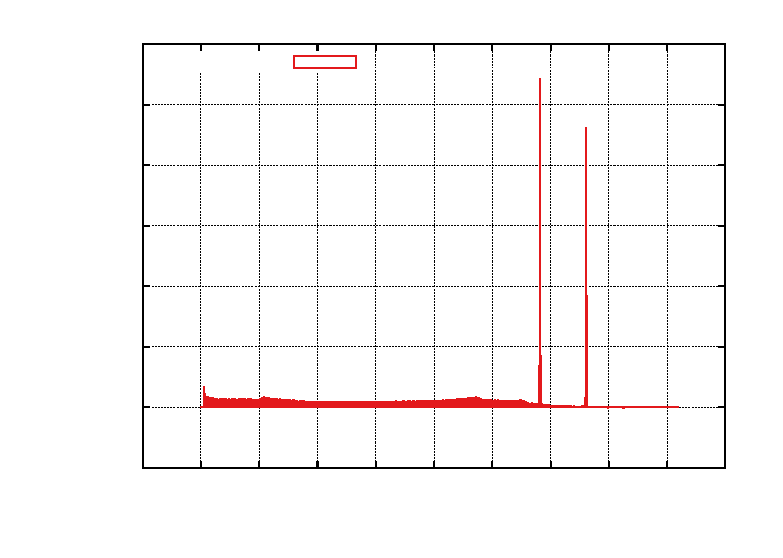
\includegraphics{./plots/halbleiter/cobalt}}%
    \gplfronttext
  \end{picture}%
\endgroup

\end{figure}

\begin{figure}
	% GNUPLOT: LaTeX picture with Postscript
\begingroup
  \makeatletter
  \providecommand\color[2][]{%
    \GenericError{(gnuplot) \space\space\space\@spaces}{%
      Package color not loaded in conjunction with
      terminal option `colourtext'%
    }{See the gnuplot documentation for explanation.%
    }{Either use 'blacktext' in gnuplot or load the package
      color.sty in LaTeX.}%
    \renewcommand\color[2][]{}%
  }%
  \providecommand\includegraphics[2][]{%
    \GenericError{(gnuplot) \space\space\space\@spaces}{%
      Package graphicx or graphics not loaded%
    }{See the gnuplot documentation for explanation.%
    }{The gnuplot epslatex terminal needs graphicx.sty or graphics.sty.}%
    \renewcommand\includegraphics[2][]{}%
  }%
  \providecommand\rotatebox[2]{#2}%
  \@ifundefined{ifGPcolor}{%
    \newif\ifGPcolor
    \GPcolortrue
  }{}%
  \@ifundefined{ifGPblacktext}{%
    \newif\ifGPblacktext
    \GPblacktexttrue
  }{}%
  % define a \g@addto@macro without @ in the name:
  \let\gplgaddtomacro\g@addto@macro
  % define empty templates for all commands taking text:
  \gdef\gplbacktext{}%
  \gdef\gplfronttext{}%
  \makeatother
  \ifGPblacktext
    % no textcolor at all
    \def\colorrgb#1{}%
    \def\colorgray#1{}%
  \else
    % gray or color?
    \ifGPcolor
      \def\colorrgb#1{\color[rgb]{#1}}%
      \def\colorgray#1{\color[gray]{#1}}%
      \expandafter\def\csname LTw\endcsname{\color{white}}%
      \expandafter\def\csname LTb\endcsname{\color{black}}%
      \expandafter\def\csname LTa\endcsname{\color{black}}%
      \expandafter\def\csname LT0\endcsname{\color[rgb]{1,0,0}}%
      \expandafter\def\csname LT1\endcsname{\color[rgb]{0,1,0}}%
      \expandafter\def\csname LT2\endcsname{\color[rgb]{0,0,1}}%
      \expandafter\def\csname LT3\endcsname{\color[rgb]{1,0,1}}%
      \expandafter\def\csname LT4\endcsname{\color[rgb]{0,1,1}}%
      \expandafter\def\csname LT5\endcsname{\color[rgb]{1,1,0}}%
      \expandafter\def\csname LT6\endcsname{\color[rgb]{0,0,0}}%
      \expandafter\def\csname LT7\endcsname{\color[rgb]{1,0.3,0}}%
      \expandafter\def\csname LT8\endcsname{\color[rgb]{0.5,0.5,0.5}}%
    \else
      % gray
      \def\colorrgb#1{\color{black}}%
      \def\colorgray#1{\color[gray]{#1}}%
      \expandafter\def\csname LTw\endcsname{\color{white}}%
      \expandafter\def\csname LTb\endcsname{\color{black}}%
      \expandafter\def\csname LTa\endcsname{\color{black}}%
      \expandafter\def\csname LT0\endcsname{\color{black}}%
      \expandafter\def\csname LT1\endcsname{\color{black}}%
      \expandafter\def\csname LT2\endcsname{\color{black}}%
      \expandafter\def\csname LT3\endcsname{\color{black}}%
      \expandafter\def\csname LT4\endcsname{\color{black}}%
      \expandafter\def\csname LT5\endcsname{\color{black}}%
      \expandafter\def\csname LT6\endcsname{\color{black}}%
      \expandafter\def\csname LT7\endcsname{\color{black}}%
      \expandafter\def\csname LT8\endcsname{\color{black}}%
    \fi
  \fi
    \setlength{\unitlength}{0.0500bp}%
    \ifx\gptboxheight\undefined%
      \newlength{\gptboxheight}%
      \newlength{\gptboxwidth}%
      \newsavebox{\gptboxtext}%
    \fi%
    \setlength{\fboxrule}{0.5pt}%
    \setlength{\fboxsep}{1pt}%
\begin{picture}(7200.00,5040.00)%
    \gplgaddtomacro\gplbacktext{%
      \csname LTb\endcsname%
      \put(946,704){\makebox(0,0)[r]{\strut{}$0$}}%
      \csname LTb\endcsname%
      \put(946,1286){\makebox(0,0)[r]{\strut{}$200$}}%
      \csname LTb\endcsname%
      \put(946,1867){\makebox(0,0)[r]{\strut{}$400$}}%
      \csname LTb\endcsname%
      \put(946,2449){\makebox(0,0)[r]{\strut{}$600$}}%
      \csname LTb\endcsname%
      \put(946,3030){\makebox(0,0)[r]{\strut{}$800$}}%
      \csname LTb\endcsname%
      \put(946,3612){\makebox(0,0)[r]{\strut{}$1000$}}%
      \csname LTb\endcsname%
      \put(946,4193){\makebox(0,0)[r]{\strut{}$1200$}}%
      \csname LTb\endcsname%
      \put(946,4775){\makebox(0,0)[r]{\strut{}$1400$}}%
      \csname LTb\endcsname%
      \put(1078,484){\makebox(0,0){\strut{}$0$}}%
      \csname LTb\endcsname%
      \put(2223,484){\makebox(0,0){\strut{}$1000$}}%
      \csname LTb\endcsname%
      \put(3368,484){\makebox(0,0){\strut{}$2000$}}%
      \csname LTb\endcsname%
      \put(4513,484){\makebox(0,0){\strut{}$3000$}}%
      \csname LTb\endcsname%
      \put(5658,484){\makebox(0,0){\strut{}$4000$}}%
      \csname LTb\endcsname%
      \put(6803,484){\makebox(0,0){\strut{}$5000$}}%
    }%
    \gplgaddtomacro\gplfronttext{%
      \csname LTb\endcsname%
      \put(176,2739){\rotatebox{-270}{\makebox(0,0){\strut{}Ereignisse $N$}}}%
      \put(3940,154){\makebox(0,0){\strut{}Kanal $n$}}%
      \csname LTb\endcsname%
      \put(5816,4602){\makebox(0,0)[r]{\strut{}Messwerte}}%
    }%
    \gplbacktext
    \put(0,0){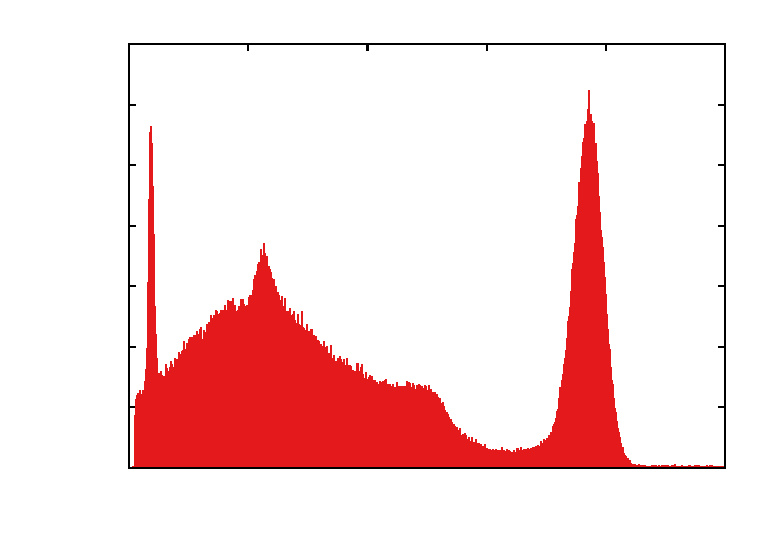
\includegraphics{./plots/szintillator/caesium}}%
    \gplfronttext
  \end{picture}%
\endgroup

\end{figure}

\FloatBarrier
% BIBLIOGRAPHIE
\vspace{\fill}
% Maximale Anzahl der Einträge in Klammer
% Zitieren mit \cite{lamport94}
\begin{thebibliography}{19}
\bibitem{siegbahn}
	K. Siegbahn,
	\emph{Alpha-, Beta- and Gamma-Ray Spectroscopy},
	Elsevier Science Ltd. 1965

\bibitem{anleitung}
	Physikalisches Praktikum V: Kern- und Teilchenphysik,
	Versuchsbeschreibung \emph{P523: $\beta$-Spektrometer} (Stand: Januar 2015),
	Universität Bonn	

\bibitem{riezler}
	Riezler, W.; Kopitzki, K.
	\emph{Kernphysikalisches Praktikum},
	Teubner 1963

\bibitem{nist}
	M. P. Unterweger, D. D. Hoppes, F. J. Schima, J.S. Coursey,
	\emph{NIST Radionuclide Half-Life Measurements},
	\url{http://www.nist.gov/pml/data/halflife-html.cfm} (Letzter Abruf: 1. Mai 2015)

\end{thebibliography}

% APPENDIX
\begin{appendix}
\section{Anhang}
Auf den folgenden Seiten sind der Vollständigkeit halber alle gemessenen Werte sowie die jeweils zur Auswertung berechneten Werte zusammengetragen.
\clearpage

\end{appendix}

\end{document}
